\documentclass[a4paper,12pt]{article}
%\documentclass[fleqn]{article}

% ---パッケージ---
\usepackage{amsmath,amssymb}    %数式用
\usepackage{tcolorbox}   %囲み枠用(tcolorboxに変更)
\usepackage{geometry}   %余白調節
\usepackage{tikz}  % ← 図を描くためのTikZパッケージ
\geometry{margin=25mm}  %余白を少し狭く
\usetikzlibrary{decorations.pathmorphing,patterns,positioning,arrows.meta} % バネ・壁の模様
\tikzset{
  block/.style = {draw, rectangle, minimum height=2em, minimum width=3em},
  sum/.style = {draw, circle, inner sep=0pt, minimum size=5mm},
  input/.style = {coordinate},
  output/.style = {coordinate}
}
\usetikzlibrary{calc}

% --- 日本語用パッケージ ---
\usepackage{luatexja}         % 日本語表示に必要
\usepackage{luatexja-fontspec} % フォント指定用

% --- フォント指定(Overleaf標準フォント)---
\setmainjfont{IPAexMincho}  % 明朝体
%\setmainjfont{IPAexGothic}  % ゴシック体にしたい場合

% --- tcolorbox の設定 ---
\tcbset{
  colframe=black,
  colback=white,         % 本文の背景(白)
  boxrule=0.8pt,
  arc=3pt,
  outer arc=3pt,
  boxsep=4pt,
  coltitle=black,
  colbacktitle=gray!20,  % タイトルの背景(グレー)
  fonttitle=\normalsize
}

\begin{document}

\begin{titlepage}
    \centering
    \vspace*{2cm}
    {\LARGE {制御工学演習} \par}
    \vspace{1cm}
    {\Large 解答編 \par}
    \vfill
    \begin{flushright}
      \large
      作成者:Yudai\\
      2025年5月9日作成
    \end{flushright}
\end{titlepage}

% --------------- [1] --------------- 済
\begin{tcolorbox}[title={[1] 指数関数 \(x(t) =e^{at}\) をラプラス変換せよ.}]

\vspace{2mm}

\[
X(s) =\int_0^{\infty} e^{-st} e^{at} dt =
\int_0^{\infty} e^{-(s-a)t} dt =
\left[ - \frac{1}{s-a} e^{-(s-a)t}\right]_0^{\infty} 
\]

\vspace{2mm}

\quad この式の右辺第2項が収束するには:
\[
\operatorname{Re}[s-a] > 0 \quad \Leftrightarrow \quad \operatorname{Re}[s] >
\operatorname{Re}[a]
\]
\quad ゆえに,ラプラス変換の定義が成り立つ条件下で,最終的に次のようにまとめられる.

\vspace{1mm}

\[
\boxed{{\mathcal{L}[e^{at}]=\frac{1}{s-a}} \quad (\operatorname{Re}[s] >\operatorname{Re}[a])}
\]

\vspace{2mm}

\end{tcolorbox}
% --------------- [2] --------------- 済
\begin{tcolorbox}[title={[2] 単位ステップ関数 \( x(t) = 1 \) をラプラス変換せよ.}]

  \vspace{4mm}
  
  \quad 単位ステップ関数の時間的変化を表しており,
  \( t < 0 \)において \( x(t) =0 \) である.単位ステップ関数を \( u(t) \) と表すことがある.
  
  \[
  X(s) = \int_0^{\infty} e^{-st} dt = 
  \left[ \frac{-1}{s} e^{-st} \right]_0^{\infty} =
  \frac{1}{s} - \lim_{t \to \infty} \frac{e^{-st}}{s} 
  \]
  
  \vspace{2mm}
  
  \begin{minipage}[t]{0.6\linewidth}
      \begin{align*}
      &\text{Re}[s] > 0 \quad \text{の定義域において収束.} \\
      &\hspace{20mm}\mathcal{L}[u(t)] = \mathcal{L}[1] = \frac{1}{s} \\
      \end{align*}
  \end{minipage}
  \hfill
  \begin{minipage}[t]{0.35\linewidth}
  \vspace{1mm}
  \begin{center}
      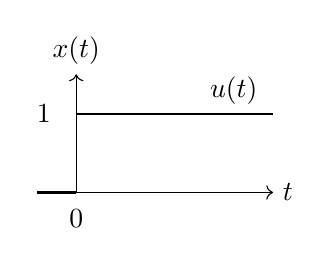
\begin{tikzpicture}
          \draw[->] (-0.5,0) -- (2.5,0) node[right] {$t$};
          \draw[->] (0,0) -- (0,1.5) node[above] {$x(t)$};
  
          \draw[thick] (-0.5,0) -- (0,0);
          \draw[thick] (0,1) -- (2.5,1);
          \draw[dashed] (0,0) -- (0,1);
  
          \node at (-0.2,1) [left] {$1$};
          \node at (0,-0.1) [below] {$0$};
          \node at (2,1) [above] {$u(t)$};
      \end{tikzpicture}\\
      図:単位ステップ関数
  \end{center}
  \end{minipage}
  
  \vspace{2mm}
  
\end{tcolorbox}
% --------------- [3] --------------- 済
\begin{tcolorbox}[title={[3] 単位インパルス関数 \( x(t) = \delta(t) \)をラプラス変換せよ.}]

  \vspace{4mm}
  
  \quad 単位ステップ関数はディラックのデルタ関数ともよばれ,\( \delta(t) \) で記述される.\\
  \quad \(h\)をゼロに近づけることで定義され,その面積では1である.
  
  \vspace{-4mm}
  
  \begin{minipage}[t]{0.6\linewidth}
      \begin{align*}
          &\quad \mathcal \int_{-\infty}^{\infty} \delta(t) dt = 1 \\[2mm]
          &\text{単位インパルス関数には次のような性質がある} \\[2mm]
          &\quad \mathcal \int_{-\infty}^{\infty} f(t)\delta(t-a) dt = f(a) \\[2mm]
          &\mathrm{Re}[s] > 0 \quad \text{の定義域において} \\[2mm]
          &\quad \mathcal{L}[u(t)] = \mathcal \int_{-\infty}^{\infty} e^{-st}\delta(t-0) dt = e^0=1\\
      \end{align*}
  \end{minipage}
  \hfill
  \begin{minipage}[t]{0.35\linewidth}
  \vspace{10mm}
  \begin{center}
      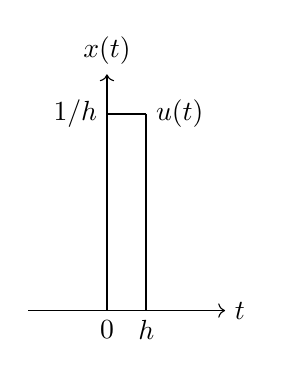
\begin{tikzpicture}
          \draw[->] (-1.0,0) -- (1.5,0) node[right] {$t$};
          \draw[->] (0,0) -- (0,3) node[above] {$x(t)$};
  
          \draw[thick] (0,2.5) -- (0.5,2.5);
          \draw[thick] (0.5,2.5) -- (0.5,0);
  
          \node at (0,2.5) [left] {$1/h$};
          \node at (0,0) [below] {$0$};
          \node at (0.5,0) [below] {$h$};
          \node at (0.5,2.5) [right] {$u(t)$};
      \end{tikzpicture}\\
      図:単位インパルス関数
  \end{center}
  \end{minipage}
  
\end{tcolorbox}
% --------------- [4] --------------- 済
\begin{tcolorbox}[title={[4] ランプ関数 \( x(t) = t \) をラプラス変換せよ.}]

  \begin{minipage}{0.6\linewidth}
  \begin{align*}
  X(s) &= \int_0^{\infty} te^{-st} dt \\
  &=\left[ t \left( - \frac{1}{s}e^{-st} \right) \right]_0^{\infty} - 
  \int_0^{\infty} \left( -\frac{1}{s}e^{-st} \right) dt \\
  &=0 + \frac{1}{s} \int_{0}^{\infty} e^{-st} \\
  &=\frac{1}{s} \mathcal{L} \left[ 1 \right] \\
  &=\frac{1}{s^2}
  \end{align*}
  \end{minipage}
  \hfill
  \begin{minipage}{0.35\linewidth}
  \begin{center}
      \begin{tikzpicture}
          \draw[->] (-0.5,0) -- (2.5,0) node[right] {$t$};
          \draw[->] (0,0) -- (0,2.5) node[above] {$x(t)$};
  
          \draw[thick] (0,0) -- (2,2);
          \draw[dashed] (1,0) -- (1,1);
          \draw[dashed] (0,1) -- (1,1);
  
          \node at (0,1) [left] {$1$};
          \node at (0,0) [below] {$0$};
          \node at (1,0) [below] {$h$};
      \end{tikzpicture}\\
      図:ランプ関数
  \end{center}
  \end{minipage}
  
\end{tcolorbox}
% --------------- [5] --------------- 済
\begin{tcolorbox}[title={[5] 正弦波関数 \( x(t) = \sin(\omega t) \) をラプラス変換せよ.}]
  
  \quad オイラーの等式より
  \begin{align*}
  \left\{
      \begin{aligned}
          e^{j \omega t} &= \cos(\omega t) + j \sin(\omega t) \\
          e^{-j \omega t} &= \cos(\omega t) - j \sin(\omega t)
      \end{aligned}
  \right.
  \end{align*}
  
  \vspace{-2mm}
  
  \begin{align*}
  \mathcal{L} \left[ \sin(\omega t) \right] &=
  \mathcal{L} \left[ \frac{1}{2j}\left( e^{j \omega t} - e^{-j \omega t} \right) \right] \\
  &=\frac{1}{2j} \left( \frac{1}{s-j \omega} - \frac{1}{s + j \omega} \right) \\
  &=\frac{1}{2j} \cdot \frac{2j\omega}{s^2 + \omega^2} \\
  &=\frac{\omega}{s^2 + \omega^2}
  \end{align*}
  
\end{tcolorbox}
% --------------- [6] --------------- 済
\begin{tcolorbox}[title={[6] 余弦波関数 \( x(t) = \cos(\omega t) \) をラプラス変換せよ.}]
  
  \quad [5]と同様にして
  \vspace{-2mm}
  \begin{align*}
  \mathcal{L} \left[ \cos(\omega t) \right] &=
  \mathcal{L} \left[ \frac{1}{2}\left( e^{j \omega t} + e^{-j \omega t} \right) \right] \\
  &=\frac{1}{2} \left( \frac{1}{s-j \omega} + \frac{1}{s + j \omega} \right) \\
  &=\frac{1}{2} \cdot \frac{2s}{s^2 + \omega^2} \\
  &=\frac{s}{s^2 + \omega^2}
  \end{align*}
  
\end{tcolorbox}
% --------------- [7] --------------- 済
\begin{tcolorbox}[title={[7] ラプラス変換は線形の性質があることを示せ. }]

  %左:数式

  \quad 線形の性質
  \vspace{-3mm}
  \begin{align*}
      \left\{
          \begin{aligned}
          \mathcal{L} \left[ x_{1}(t) + x_{2}(t) \right] &=
          \mathcal{L} \left[ x_{1}(t)  \right] +
          \mathcal{L} \left[ x_{2}(t)  \right] \\
          \mathcal{L} \left[ a x_{1}(t)  \right] &=
          a \mathcal{L} \left[ x_{1}(t)  \right] \\
          \end{aligned}
      \right.
  \end{align*}

  \quad を示す.
  \vspace{-3mm}

  \begin{align*}
      \mathcal{L} \left[ a x_{1}(t) + b x_{2}(t) \right] &=
      \int_{0}^{\infty} \left\{ a x_{1}(t) + b x_{2}(t) \right\} e^{-st} dt \\
      &=a \int_{0}^{\infty} x_{1}(t) e^{-st} dt + b \int_{0}^{\infty} x_{2}(t) e^{-st} dt \\
      &=a \mathcal{L} \left[ x_{1}(t)  \right] +
      b \mathcal{L} \left[ x_{2}(t)  \right] \\
  \end{align*}



\vspace{2mm}
  \end{tcolorbox}
% --------------- [8] --------------- 済
\begin{tcolorbox}[title={[8] 時間関数\( x(t) \)を右に \tau だけ推移させた関数\( x(t - \tau) \)に対するラプラス変換は,\\
  \quad \( x(t) \) のラプラス変換 \( X(s)\) を用いて 
  \vspace{-2mm}
\begin{align*}
    \mathcal{L} \left[ x(t - \tau) \right] &=
    e^{-s
    \tau t}X(s)
\end{align*}
\quad と表されることを示せ.(時間領域における推移定理)
  }]

  \vspace{-6mm}
\begin{minipage}{0.6\linewidth}
    \begin{align*}
        \mathcal{L} \left[ x(t - \tau) \right] &=
        \int_{0}^{\infty} x( t - \tau ) e^{-st} dt \\
        &= \int_{\tau}^{\infty} x( t - \tau ) e^{-st} dt \\ 
        &\quad [\because t < \tau の時 \quad x( t - \tau ) = 0 ]\\
    \end{align*}

    \vspace{-6mm}
    \quad ここで変数変換\tau' = t - \tau を行う.

    \vspace{-6mm}
    \begin{align*}
        \mathcal{L} \left[ x(t - \tau) \right] &=
        \int_{0}^{\infty - \tau} x( \tau' ) e^{-s( \tau +\tau')} d\tau' \\
        &=e^{-\tau s} \int_{0}^{\infty} x( \tau' ) e^{-s\tau'} d\tau' \\
        &= e^{-\tau s} \mathcal{L} \left[ x( t ) \right] \\
        &= e^{-\tau s} X(s)
    \end{align*}

\end{minipage}
\hfill
%右:図
\begin{minipage}{0.35\linewidth}
    \centering
    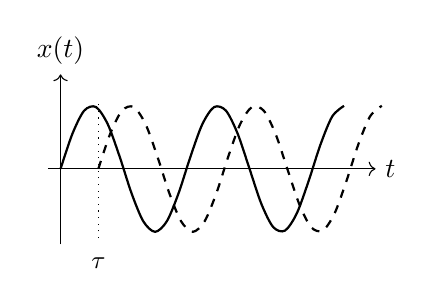
\begin{tikzpicture}[scale=0.8]
        % 軸
        \draw[->] (-0.2,0) -- (5.0,0) node[right] {$t$};
        \draw[->] (0,-1.2) -- (0,1.5) node[above] {$x(t)$};
    
        % パラメータ
        \def\w{180}      % 度数法での1周期 = π
        \def\taushift{0.6}  % τ のシフト値
        
        % x(t)
        \draw[domain=0:4.5,smooth,variable=\t,thick]
            plot ({\t},{sin(\w*\t)});
        
        % x(t - τ)
        \draw[domain=\taushift:5.1,smooth,variable=\t,thick,dashed]
            plot ({\t},{sin(\w*(\t-\taushift))});
        
        % τの線とラベル
        \draw[dotted] (\taushift,-1.1) -- (\taushift,1.1);
        \node at (\taushift,-1.5) {\small $\tau$};
    
    \end{tikzpicture}
    % グラフ下の凡例(線+式)
    \vspace{0.5em}
    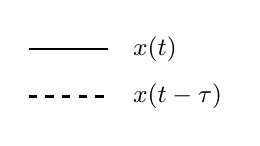
\begin{tikzpicture}
        % 実線とそのラベル
        \draw[thick] (0,0) -- (1,0);
        \node[right] at (1.2,0) {\small $x(t)$};

        % 破線とそのラベル
        \draw[thick, dashed] (0,-0.6) -- (1,-0.6);
        \node[right] at (1.2,-0.6) {\small $x(t - \tau)$};
    \end{tikzpicture}

    図:時間領域における推移
\end{minipage}

\vspace{2mm}
  \end{tcolorbox}
% --------------- [9] --------------- 済
\begin{tcolorbox}[title={[9]  \( x(t) \) のラプラス変換\( X(s) \)において複素変数\(s\)を\(b\)だけ推移させて \(s+b\) \\
  \quad とすれば,どうなるのか? }]

  \vspace{-3mm}
  \begin{align*}
  X(s+b) &= \int_0^{\infty} x(t) e^{-\left( s + b \right)t} dt \\
  &= \int_0^{\infty} \left\{ e^{-bt} x(t) \right\} e^{-st} dt \\
  &= \mathcal{L} \left[ e^{-bt} x(t) \right]
  \end{align*}


\vspace{2mm}
  \end{tcolorbox}
% --------------- [10] ---------------済
\begin{tcolorbox}[title={[10] \( e^{\lambda t} sin(\omega t) \) をラプラス変換せよ. }]

  \quad ラプラス変換の第一移動定理(問題[8])

  \[
      \mathcal{L} \left[ e^{at} f(t) \right] = F(s - a)
  \]

  と,正弦波のラプラス変換(問題[5])

  \[
      \mathcal{L} \left[ sin(\omega t) \right] = \frac{\omega}{ s^2+ {\omega}^2} \quad \left( = X(s) \right)
  \]

  を考えれば,


  \vspace{-3mm}
  \begin{align*}
      \mathcal{L} \left[ e^{\lambda t} sin(\omega t) \right] &=
      X(s - \lambda) \\
      &=\frac{\omega}{ \left(s - \lambda \right)^2+ {\omega}^2}
  \end{align*}

  \vspace{2mm}
\vspace{2mm}
  \end{tcolorbox}
% --------------- [11] --------------- 済
\begin{tcolorbox}[title={[11] 時間関数 \( x(t) \) の微分をラプラス変換せよ. }]

  \begin{align*}
    \mathcal{L} \left[ \frac{dx(t)}{dt} \right] 
    &= \int_0^{\infty} \frac{dx(t)}{dt} e^{-st} dt \\
    &= \left[ x(t) e^{-st} \right]_{0}^{\infty}
    + s \int_0^{\infty} x(t) e^{-st} dt
\end{align*}

\quad \( \displaystyle \lim_{t \to \infty} x(t) e^{- \sigma t} = 0 \) となる\( \sigma < Re[s] \) において

\[
    \mathcal{L} \left[ \frac{dx(t)}{dt} \right] = sX(s) - x(0)
\]

\vspace{2mm}




\vspace{2mm}
  \end{tcolorbox}
% --------------- [12] --------------- 済
\begin{tcolorbox}[title={[12] つぎの微分方程式をラプラス変換を用いて解け.
  \[
      9 \frac{d^2 x(t)}{dt^2} + x(t) = 1 
  \]
  \quad ただし,初期値は,$x(0) = 0,\ x'(0) = 0$ とする.
  }]

  \quad まず,時間関数 \( x(t) \) の二階微分のラプラス変換は\( \mathcal{L} \left[ \frac{dx(t)}{dt} \right] = sX(s) - x(0) \)より,
    \vspace{-3mm}
    \begin{align*}
        \mathcal{L} \left[ \frac{d^2x(t)}{dt^2} \right] 
        &= s \mathcal{L} \left[ \frac{dx(t)}{dt} \right] - x'(0) \\
        &= s \left\{ sX(s) - x(0) \right\} - x'(0) \\
        &= s^2 X(s) - s x(0) - x'(0)
    \end{align*}


\newpage

\quad 両辺にラプラス変換を施すと,

\vspace{-6mm}

\begin{align*}
    &\qquad 9 \mathcal{L} \left[ \frac{d^2 x(t)}{dt^2} \right] + \mathcal{L}[x(t)] = \mathcal{L}[1] \\
    &\Leftrightarrow \quad 9\left\{s^2 X(s) - s x(0) - x'(0)\right\} + X(s) = \frac{1}{s} \\
    &\Leftrightarrow \quad 9s^2 X(s) + X(s) = \frac{1}{s} \\
    &\Leftrightarrow \quad (9s^2 + 1) X(s) = \frac{1}{s} \\
    &\Leftrightarrow \quad X(s) = \frac{1}{s(9s^2 + 1)} \\
    &\Leftrightarrow \quad X(s)= \frac{(\frac{1}{3})^2}{s(s^2 + \left( \frac{1}{3} \right)^2)} \\
    &\Leftrightarrow \quad X(s)= \frac{\omega^2}{s(s^2 + \omega^2)} \quad \left[\because \omega = \frac{1}{3} \text{とおいた}\right]\\
    &\Leftrightarrow \quad X(s)= \frac{\omega^2}{s(s + j \omega)(s - j \omega)} \\
    &\Leftrightarrow \quad X(s)= \frac{1}{s} - \frac{\frac{1}{2}}{s + j \omega} - \frac{\frac{1}{2}}{s - j \omega} \quad \left[ \because ヘヴィサイドの展開定理 \right]
\end{align*}

\quad 両辺にラプラス逆変換を施すと,

\vspace{-6mm}

\begin{align*}
    &\qquad  \mathcal{L}^{-1} \left[ X(s) \right]
    = \mathcal{L}^{-1} \left[ \frac{1}{s} \right] 
    - \frac{1}{2} \mathcal{L}^{-1} \left[\frac{1}{s + j \omega} \right]
    - \frac{1}{2} \mathcal{L}^{-1} \left[\frac{1}{s - j \omega} \right] \\
    &\Leftrightarrow \quad x(t) 
    = 1 - \frac{1}{2} e^{-j \omega t} - \frac{1}{2} e^{j \omega t} \\
    &\Leftrightarrow \quad x(t) 
    = 1 - \frac{1}{2} \left( e^{-j \omega t} + e^{j \omega t} \right) \\
    &\Leftrightarrow \quad x(t) 
    = 1 - cos{\omega t} \quad \left[ \because オイラーの等式 \right]\\
    &\Leftrightarrow \quad x(t) 
    = 1 - cos \left(\frac{t}{3}\right)
\end{align*}



\vspace{2mm}
  \end{tcolorbox}
% --------------- [13] --------------- 済
\begin{tcolorbox}[title={[13] つぎの微分方程式をラプラス変換を用いて解け.
  \[
  \frac{d^2 x(t)}{dt^2} + 3 \frac{dx(t)}{dt} + 2x(t) = 4
  \]
  \quad ただし,初期条件は,$x(0)=1,\ x^{(1)}(0)=0$ とする. }]

  \quad 両辺にラプラス変換を施すと,
\vspace{-3mm}
\begin{align*}
&\quad \mathcal{L} \left[ \frac{d^2 x(t)}{dt^2} + 3 \frac{dx(t)}{dt} + 2x(t) \right]
= \mathcal{L} \left[ 4 \right] \\
&\Leftrightarrow \left\{s^2 X(s) - sx(0)\right\} - x^{(1)}(0) + 3\left\{sX(s) - x(0) \right\} + 2X(s) = \frac{4}{s} \\
&\Leftrightarrow s^2 X(s) + 3sX(s) + 2X(s) = \frac{4}{s} + s + 3 \\
&\Leftrightarrow X(s) = \frac{\frac{4}{s} + s + 3}{s^2 + 3s + 2} = \frac{4 + s(s + 3)}{s(s + 1)(s + 2)} = \frac{s^2 + 3s + 4}{s(s + 1)(s + 2)} \\
&\Leftrightarrow X(s) = \frac{2}{s} - \frac{2}{s+1} + \frac{1}{s+2} \quad \left[ \because ヘヴィサイドの展開定理 \right]
\end{align*}

\quad 両辺にラプラス逆変換を施すと,
\vspace{-3mm}
\begin{align*}
&\quad \mathcal{L}^{-1} \left[ X(s) \right] 
= \mathcal{L}^{-1} \left[ \frac{2}{s} - \frac{2}{s+1} + \frac{1}{s+2} \right] \\
&\Leftrightarrow x(t) = 2 - 2e^{-t} + e^{-2t}
\end{align*}



\vspace{2mm}
  \end{tcolorbox}
% --------------- [14] --------------- 済
\begin{tcolorbox}[title={[14] つぎの微分方程式をラプラス変換を用いて解け.\\
  \[
  \frac{dx(t)}{dt} + 3x(t) = sin{2t}
  \]
  
  \quad ただし,初期条件は,$x(0)=0$ とする. }]

  \quad 両辺にラプラス変換を施すと,
  \begin{align*}
      &\qquad \mathcal{L}\left[\frac{dx(t)}{dt} + 3\mathcal{L} x(t)\right] = \mathcal{L}\{\sin 2t\} \\
      &\Leftrightarrow sX(s) - x(0) + 3X(s) = \frac{2}{s^2 + 4} \\
      &\Leftrightarrow sX(s) + 3X(s) = \frac{2}{s^2 + 4} \\
      &\Leftrightarrow X(s) = \frac{2}{(s+3)(s^2 + 4)}  \\
      &\Leftrightarrow X(s)= \frac{2}{13} \left( \frac{1}{s+3} + \frac{3}{s^2 + 4} - \frac{s}{s^2 + 4} \right) 
      \quad \left[ \because ヘヴィサイドの展開定理 \right]
  \end{align*}
      
  \quad 両辺にラプラス逆変換を施すと,
  \vspace{-3mm}
  \begin{align*}
  &\quad \mathcal{L}^{-1} \left[ X(s) \right] 
  = \mathcal{L}^{-1} \left[ \frac{2}{13} \left( \frac{1}{s+3} + \frac{3}{s^2 + 4} - \frac{s}{s^2 + 4} \right) \right] \\
  &\Leftrightarrow x(t) = \frac{1}{13} \left( 2e^{-3t} + 3\sin 2t - 2\cos 2t \right)
  \end{align*}
  


\vspace{2mm}
  \end{tcolorbox}
% --------------- [15] --------------- 済
\begin{tcolorbox}[title={[15] つぎの微分方程式をラプラス変換を用いて解け.\\
  \[
  \frac{d^2 x(t)}{dt^2} + 2\frac{dx(t)}{dt} + 2x(t) = 1 \\
  \]
  
  \quad ただし,初期条件は,$x(0)=0 , x^{1}(0)=1$ とする. }]

  \quad 両辺にラプラス変換を施すと,
\begin{align*}
    &\qquad \mathcal{L}\left[ \frac{d^2 x(t)}{dt^2} + 2 \frac{dx(t)}{dt} + 2x(t) \right] = \mathcal{L}\{1\} \\
    &\Leftrightarrow \left\{s^2 X(s) - sx(0) - x^{(1)}(0) \right\} 
    + 2 \left\{ sX(s) - x(0) \right\} + 2X(s) 
    = \frac{1}{s} \\
    &\Leftrightarrow s^2 X(s) - 1 + 2sX(s) + 2X(s) = \frac{1}{s} \\
    &\Leftrightarrow s^2 X(s) + 2sX(s) + 2X(s) = \frac{1}{s} + 1 \\
    &\Leftrightarrow X(s) = \frac{1}{s(s^2 + 2s + 2)} + \frac{1}{s^2 + 2s + 2} \\
    &\Leftrightarrow X(s) = \frac{1}{2} \left\{ \frac{1}{s} - \frac{s+1}{(s+1)^2 + 1^2} + \frac{1}{(s+1)^2 + 1^2} \right\}
\end{align*}
\qquad 両辺にラプラス逆変換を施すと,
    \vspace{-3mm}
\begin{align*}
    \mathcal{L}^{-1}\{X(s)\} = \frac{1}{2} \left\{ 1 - e^{-t}(\cos t - \sin t) \right\}
\end{align*}



\vspace{2mm}
  \end{tcolorbox}

\newpage
% --------------- [16] ---------------

[16] (1)-(10)のラプラス変換$X(s)$にラプラス逆変換を施し,時間関数$x(t)$を求めよ.\\


% --------------- [16-1] --------------- 済
\begin{tcolorbox}[title={ [16] (1) \( X(s)=\frac{4}{s+5} \)}]
  \quad 両辺にラプラス逆変換を施すと,
\vspace{-3mm}
\begin{align*}
    &\qquad \mathcal{L}^{-1} \left[ X(s) \right] 
    =\mathcal{L}^{-1} \left[ \frac{4}{s+5} \right] \\
    &\Leftrightarrow x(t) = 4 e^{-5t}
\end{align*}
\end{tcolorbox}
% --------------- [16-2] --------------- 済
\begin{tcolorbox}[title={ [16] (2) \( X(s)=\frac{ s + 7 }{ s^2 + 2s + 5} \)}]
  \vspace{-3mm}
\begin{align*}
    &\qquad X(s) =\frac{ s + 7 }{ s^2 + 2s + 5}  \\
    &\Leftrightarrow X(s) =\frac{ (s + 1) + 6 }{ ( s + 1 )^2+ 2^2} \\
    &\Leftrightarrow X(s) 
    = \frac{ (s + 1) }{ ( s + 1 )^2+ 2^2}
    + \frac{ 6 }{ ( s + 1 )^2+ 2^2} 
\end{align*}

\quad 両辺にラプラス逆変換を施すと,
\vspace{-3mm}
\begin{align*}
    &\qquad \mathcal{L}^{-1} \left[ X(s) \right] 
    =\mathcal{L}^{-1} \left[ \frac{ (s + 1) }{ ( s + 1 )^2+ 2^2} \right]
    +\mathcal{L}^{-1} \left[ \frac{ 6  }{ ( s + 1 )^2+ 2^2} \right] \\
    &\Leftrightarrow x(t) = e^{-t} cos(2t) +3 e^{-t} sin(2t)
\end{align*}
\end{tcolorbox}
% --------------- [16-3] --------------- 済
\begin{tcolorbox}[title={ [16] (3) \( X(s)=\frac{ 2 }{ s^2 + s } \)}]
  \vspace{-3mm}
\begin{align*}
    &\qquad X(s) =\frac{ 2 }{ s^2 + s }  \\
    &\Leftrightarrow X(s) =\frac{ 2 }{ s(s+1) }  \\
    &\Leftrightarrow X(s) 
    = \frac{2}{s}
    + \frac{-2}{s + 1} 
    \quad [\because ヘヴィサイドの展開定理]
\end{align*}

\quad 両辺にラプラス逆変換を施すと,
\vspace{-3mm}
\begin{align*}
    &\qquad \mathcal{L}^{-1} \left[ X(s) \right] 
    =\mathcal{L}^{-1} \left[ \frac{2}{s} \right]
    -\mathcal{L}^{-1} \left[ \frac{2}{s + 1} \right] \\
    &\Leftrightarrow x(t) = 2 - 2 e^{-t}
\end{align*}\end{tcolorbox}
% --------------- [16-4] --------------- 済
\begin{tcolorbox}[title={ [16] (4) \( X(s)=\frac{ s + 1 }{ s ( s^2 + 4s + 8 ) } \)}]
  \vspace{-3mm}
\begin{align*}
    &\qquad X(s) =\frac{ s + 1 }{ s ( s^2 + 4s + 8 ) }  \\
    &\Leftrightarrow X(s) 
    = \frac{ \frac{1}{8} }{s}
    +\frac{ -\frac{1}{8}(s-4) }{ s^2 + 4s + 8 } 
    \quad [\because ヘヴィサイドの展開定理]\\
    &\Leftrightarrow X(s) 
    =\frac{1}{8s}
    -\frac{ (s+2)-6}{8\left\{(s+2)^2 + 4 \right\}}
\end{align*}

\quad 両辺にラプラス逆変換を施すと,
\vspace{-3mm}
\begin{align*}
    &\qquad \mathcal{L}^{-1} \left[ X(s) \right] 
    =\mathcal{L}^{-1} \left[ \frac{1}{8s} \right]
    -\mathcal{L}^{-1} \left[ \frac{ (s+2)-6}{8\left\{(s+2)^2 + 4 \right\}} \right] \\
    &\Leftrightarrow x(t) = \frac{1}{8} - \frac{1}{8}e^{-2t}(cos(2t)-3sin(2t))
\end{align*}
\end{tcolorbox}
% --------------- [16-5] --------------- 済
\begin{tcolorbox}[title={ [16] (5) \( X(s)=\frac{ 1 }{ s^3 + 11 s^2+ 40s + 48 } \) }]
  \vspace{-3mm}
\begin{align*}
    &\qquad X(s) =\frac{ 1 }{ s^3 + 11 s^2+ 40s + 48 }  \\
    &\Leftrightarrow X(s) =\frac{ 1 }{ (s+3)(s+4)^2 }  \\
    &\Leftrightarrow X(s) 
    = \frac{1}{s+3}
    + \frac{-1}{s + 4}
    + \frac{-1}{(s + 4)^2}
    \quad [\because ヘヴィサイドの展開定理]
\end{align*}

\quad 両辺にラプラス逆変換を施すと,
\vspace{-3mm}
\begin{align*}
    &\qquad \mathcal{L}^{-1} \left[ X(s) \right] 
    =\mathcal{L}^{-1} \left[ \frac{1}{s+3} \right]
    +\mathcal{L}^{-1} \left[ \frac{-1}{s + 4} \right]
    +\mathcal{L}^{-1} \left[ \frac{-1}{(s + 4)^2} \right] \\
    &\Leftrightarrow x(t) = e^{-3t} - e^{-4t} - te^{-4t}
\end{align*}
\end{tcolorbox}
% --------------- [16-6] --------------- 済
\begin{tcolorbox}[title={ [16] (6) \( X(s)=\frac{ 2 }{ ( s + 1 ) ( s + 3 ) } \)}]
  \vspace{-3mm}
\begin{align*}
    &\qquad X(s) =\frac{ 2 }{ ( s + 1 ) ( s + 3 ) }  \\
    &\Leftrightarrow X(s) 
    = \frac{1}{s + 1}
    + \frac{-1}{s + 3} 
    \quad [\because ヘヴィサイドの展開定理]
\end{align*}

\quad 両辺にラプラス逆変換を施すと,
\vspace{-3mm}
\begin{align*}
    &\qquad \mathcal{L}^{-1} \left[ X(s) \right] 
    =\mathcal{L}^{-1} \left[ \frac{1}{s + 1} \right]
    +\mathcal{L}^{-1} \left[ \frac{-1}{s + 3} \right] \\
    &\Leftrightarrow x(t) = e^{-t} - e^{-3t}
\end{align*}
\end{tcolorbox}
% --------------- [16-7] --------------- 済
\begin{tcolorbox}[title={ [16] (7) \( X(s)=\frac{ 3 }{ s ( s + 2)^2 } \)}]
  \vspace{-3mm}
\begin{align*}
    &\qquad X(s) =\frac{ 3 }{ s ( s + 2)^2 }  \\
    &\Leftrightarrow X(s) 
    = \frac{(\frac{3}{4})}{s}
    + \frac{(-\frac{3}{4})}{s + 1} 
    + \frac{(-\frac{3}{2})}{(s + 1)^2} 
\end{align*}

\quad 両辺にラプラス逆変換を施すと,
\vspace{-3mm}
\begin{align*}
    &\qquad \mathcal{L}^{-1} \left[ X(s) \right] 
    = \mathcal{L}^{-1} \left[\frac{(\frac{3}{4})}{s} \right]
    + \mathcal{L}^{-1} \left[ \frac{(-\frac{3}{4})}{s + 1} \right]
    + \mathcal{L}^{-1} \left[\frac{(-\frac{3}{2})}{(s + 1)^2}\right]\\
    &\Leftrightarrow x(t) = \frac{3}{4}-\frac{3}{4}e^{-2t}-\frac{3}{2}te^{-2t}
\end{align*}
\end{tcolorbox}
% --------------- [16-8] --------------- 済
\begin{tcolorbox}[title={ [16] (8) \( X(s)=\frac{ 1 }{ s ( s + 2 ) ( s + 3 )^2 } \) }]
  \vspace{-3mm}
\begin{align*}
    &\qquad X(s) =\frac{ 1 }{ s ( s + 2 ) ( s + 3 )^2 }  \\
    &\Leftrightarrow X(s) 
    = \frac{\frac{1}{18}}{s}
    + \frac{(-\frac{1}{2})}{s + 2} 
    + \frac{\frac{1}{3}}{(s + 3)^2} 
    + \frac{\frac{4}{9}}{s + 3} 
\end{align*}

\quad 両辺にラプラス逆変換を施すと,
\vspace{-3mm}
\begin{align*}
    &\qquad \mathcal{L}^{-1} \left[ X(s) \right] 
    =\mathcal{L}^{-1} \left[ \frac{\frac{1}{18}}{s} \right]
    + \mathcal{L}^{-1} \left[ \frac{(-\frac{1}{2})}{s + 2} \right]
    + \mathcal{L}^{-1} \left[ \frac{\frac{1}{3}}{(s + 3)^2} \right]
    + \mathcal{L}^{-1} \left[ \frac{\frac{4}{9}}{s + 3} \right] \\
    &\Leftrightarrow x(t) = \frac{1}{18} - \frac{1}{2}e^{-2t} + \frac{1}{3}e^{-3t} +\frac{4}{9}e^{-3t}\\
    &\Leftrightarrow x(t) =\frac{1}{18} \left(1 - 9e^{-2t} + 8e^{-3t} +6te^{-3t} \right)
\end{align*}
\end{tcolorbox}
% --------------- [16-9] --------------- 済
\begin{tcolorbox}[title={ [16] (9) \( X(s)=\frac{ s + 2 }{s^3 ( s - 1 )^2 } \) }]
  \vspace{-3mm}
\begin{align*}
    &\qquad X(s) =\frac{ s + 2 }{ ( s - 1 )^2 s^3 }  \\
    &\Leftrightarrow X(s) 
    = \frac{2}{s^3}
    + \frac{5}{s^2} 
    + \frac{8}{s}
    + \frac{3}{(s - 1)^2}
    + \frac{-8}{s - 1}
\end{align*}

\quad 両辺にラプラス逆変換を施すと,
\vspace{-3mm}
\begin{align*}
    &\qquad \mathcal{L}^{-1} \left[ X(s) \right] 
    =\mathcal{L}^{-1} \left[
        \frac{2}{s^3}
    + \frac{5}{s^2} 
    + \frac{8}{s}
    + \frac{3}{(s - 1)^2}
    + \frac{-8}{s - 1} \right] \\
    &\Leftrightarrow x(t) = \left(2t^2+5t+8\right) + \left(3t-8\right) e^{t}
\end{align*}
\end{tcolorbox}
% --------------- [16-10] --------------- 済
\begin{tcolorbox}[title={ [16] (10) \( X(s)=\frac{ 1 }{ ( s^2 + 1 ) ( s^2 + 4 ) } \) }]
  \vspace{-3mm}
  \begin{align*}
    &\qquad X(s) =\frac{ 1 }{ ( s^2 + 1 ) ( s^2 + 4 ) } \\
    &\Leftrightarrow X(s) 
    = \frac{ \frac{1}{3} }{ ( s^2 + 1 ) }
    + \frac{ -\frac{1}{3} }{ ( s^2 + 4 ) }
\end{align*}

\quad 両辺にラプラス逆変換を施すと,
\vspace{-3mm}
\begin{align*}
    &\qquad \mathcal{L}^{-1} \left[ X(s) \right] 
    =\mathcal{L}^{-1} \left[ \frac{ \frac{1}{3} }{ ( s^2 + 1 ) } \right]
    +\mathcal{L}^{-1} \left[ \frac{- \frac{1}{3} }{ ( s^2 + 4 ) } \right] \\
    &\Leftrightarrow x(t) = \frac{1}{3}sin t -\frac{1}{6}sin 2t
\end{align*}

\end{tcolorbox}
% --------------- [17] --------------- 済
\begin{tcolorbox}[title={[17] つぎの微分方程式をラプラス変換を用いて解け.\\
  \[
  \frac{d^2y(t)}{dt^2} + y(t) = 0
  \]
  
  \quad ただし,初期条件は,\(y(0)=A, y^{(1)}(0)=B\) とする. }]

  \quad 両辺にラプラス変換を施すと,
\vspace{-3mm}
\begin{align*}
    &\qquad \mathcal{L}\left[ \frac{d^2y(t)}{dt^2} + y(t) \right] = 0 \\
    &\Leftrightarrow \left\{ s^2 Y(s) - sy(0) - y^{(1)}(0) \right\} + Y(s) = 0  \\
    &\Leftrightarrow s^2 Y(s) - A s - B + Y(s) = 0  \\
    &\Leftrightarrow Y(s) = \frac{As + B}{ s^2 + 1}  \\
    &\Leftrightarrow Y(s) = \frac{As}{ s^2 + 1} + \frac{B}{ s^2 + 1} 
\end{align*}
    
\quad 両辺にラプラス逆変換を施すと,
\vspace{-3mm}
\begin{align*}
&\qquad \mathcal{L}^{-1} \left[ Y(s) \right] 
= \mathcal{L}^{-1} \left[ \frac{As}{ s^2 + 1} + \frac{B}{ s^2 + 1}  \right] \\
&\Leftrightarrow y(t) = A cos{t} + B sin{t}
\end{align*}
  \end{tcolorbox}
% --------------- [18] --------------- 済
\begin{tcolorbox}[title={[18] つぎの微分方程式をラプラス変換を用いて解け.\\
  \[
  \frac{d^2y(t)}{dt^2} -( a + b )\frac{dy(t)}{dt} + a b y(t) = 0
  \]
  
  \quad ただし,初期条件は,\(y(0)=1, y^{(1)}(0)=0\) とする.}]

  \quad 両辺にラプラス変換を施すと,
        \vspace{-3mm}
        \begin{align*}
            &\qquad \mathcal{L}\left[ \frac{d^2y(t)}{dt^2} - ( a + b )\frac{dy(t)}{dt} + a b y(t) \right] = 0 \\
            &\Leftrightarrow \left\{ s^2 Y(s) - sy(0) - y^{(1)}(0) \right\}
            - (a+b)\left\{ sY(s) - y(0) \right\}
            + abY(s) = 0  \\
            &\Leftrightarrow \left\{ s^2 - (a + b) s + ab\right\} Y(s) - s + ( a + b )= 0  \\
            &\Leftrightarrow Y(s) = \frac{s - (a + b)}{ s^2 - (a + b) s + ab }  \\
            &\Leftrightarrow Y(s) =  \frac{s - (a + b)}{ (s - a)(s - b) }  \\
            &\Leftrightarrow Y(s) =  \frac{- \frac{b}{a-b}}{ (s - a) } + \frac{ \frac{a}{a-b}}{ (s - b) }
        \end{align*}
            
        \quad 両辺にラプラス逆変換を施すと,
        \vspace{-3mm}
        \begin{align*}
        &\qquad \mathcal{L}^{-1} \left[ Y(s) \right] 
        = \mathcal{L}^{-1} \left[ \frac{- \frac{b}{a-b}}{ (s - a) } + \frac{ \frac{a}{a-b}}{ (s - b) }  \right] \\
        &\Leftrightarrow y(t) = - \frac{b}{a-b}e^{at} + \frac{a}{a-b}e^{bt}
        \end{align*}
    \end{tcolorbox}
% --------------- [19] --------------- 済
\begin{tcolorbox}[title={[19] つぎの微分方程式をラプラス変換を用いて解け.\\
  \[
  \frac{d^2y(t)}{dt^2} - \frac{dy(t)}{dt} - 12 y(t) = 2
  \]
  
  \quad ただし,初期条件は,\(y(0)=1, y^{(1)}(0)=0\) とする.}]

  \quad 両辺にラプラス変換を施すと,
    \vspace{-3mm}
    \begin{align*}
        &\qquad \mathcal{L}\left[ \frac{d^2y(t)}{dt^2} - \frac{dy(t)}{dt} - 12 y(t) \right] 
        = \mathcal{L} \left[ 2 \right] \\
        &\Leftrightarrow \left\{ s^2 Y(s) - sy(0) - y^{(1)}(0) \right\}
        - \left\{ sY(s) - y(0) \right\}
        - 12 Y(s) = \frac{2}{s}  \\
        &\Leftrightarrow \left\{ s^2 - s - 12 \right\} Y(s) - s + 1= \frac{2}{s}  \\
        &\Leftrightarrow Y(s) = \frac{s^2 - s + 2}{s(s^2 - s - 12)}  \\
        &\Leftrightarrow Y(s) =  \frac{s^2 - s + 2}{ s (s + 3)(s - 4) }  \\
        &\Leftrightarrow Y(s) =  \frac{- \frac{1}{6}}{ s } + \frac{  \frac{2}{3} }{ s + 3 } + \frac{  \frac{1}{2} }{ s - 4 } 
        \quad \left[\because ヘヴィサイドの展開定理 \right]
    \end{align*}
        
    \quad 両辺にラプラス逆変換を施すと,
    \vspace{-3mm}
    \begin{align*}
    &\qquad \mathcal{L}^{-1} \left[ Y(s) \right] 
    = \mathcal{L}^{-1} \left[ \frac{- \frac{1}{6}}{ s } + \frac{  \frac{2}{3} }{ s + 3 } + \frac{  \frac{1}{2} }{ s - 4 }  \right] \\
    &\Leftrightarrow y(t) = - \frac{1}{6} + \frac{2}{3}e^{-3t} + \frac{1}{2}e^{4t}
    \end{align*}
  \end{tcolorbox}
% --------------- [20] --------------- 済
\begin{tcolorbox}[title={[20] つぎの微分方程式をラプラス変換を用いて解け.\\
  \[
  \frac{d^2y(t)}{dt^2} + 4 y(t) = sin(t)
  \]
  
  \quad ただし,初期条件は,\(y(0)=0, y^{(1)}(0)=0\) とする. }]


    \quad 両辺にラプラス変換を施すと,
    \vspace{-3mm}
    \begin{align*}
        &\qquad \mathcal{L}\left[ \frac{d^2y(t)}{dt^2} + 4 y(t) \right] 
        = \mathcal{L} \left[ sin(t) \right] \\
        &\Leftrightarrow \left\{ s^2 Y(s) - sy(0) - y^{(1)}(0) \right\}
        + 4 Y(s) = \frac{1}{s^2 + 1}  \\
        &\Leftrightarrow \left\{ s^2 + 4 \right\} Y(s) = \frac{1}{s^2 + 1}  \\
        &\Leftrightarrow Y(s) = \frac{1}{(s^2+1)(s^2+4)}  \\
        &\Leftrightarrow Y(s) = \frac{ \frac{1}{3} }{s^2+1} - \frac{ \frac{1}{3} }{s^2+4} 
        \quad \left[\because ヘヴィサイドの展開定理 \right]
    \end{align*}
        
    \quad 両辺にラプラス逆変換を施すと,
    \vspace{-3mm}
    \begin{align*}
    &\qquad \mathcal{L}^{-1} \left[ Y(s) \right] 
    = \mathcal{L}^{-1} \left[  \frac{ \frac{1}{3} }{s^2+1} - \frac{ \frac{1}{3} }{s^2+4}   \right] \\
    &\Leftrightarrow y(t) = \frac{1}{3}sin(t) - \frac{1}{6}sin(2t)
    \end{align*}
  \end{tcolorbox}
% --------------- [21] --------------- 済
\begin{tcolorbox}[title={[21] 単位インパルス応答が\(y(t)=7e^{-2t}+2e^{-3t}\)であるとき,\\ 
    \qquad このシステムの伝達関数を求めよ. }]

    伝達関数は単位インパルス応答\(y(t)\)をラプラス変換して得ることができる.
    \begin{align*}
        \mathcal{L} \left[ y(t) \right] 
        &= 7 \mathcal{L} \left[ e^{-2t} \right]+2 \mathcal{L} \left[ e^{-3t} \right]\\
        &= \frac{7}{s+2} + \frac{2}{s+3}\\
        &= \frac{7s+21+2s+4}{(s+2)(s+3)}\\
        &= \frac{9s+25}{(s+2)(s+3)}\\
        \Leftrightarrow G(s) &= \frac{9s+25}{(s+2)(s+3)}
    \end{align*}

\end{tcolorbox}
% --------------- [22] --------------- 済
\begin{tcolorbox}[title={[22] 単位インパルス応答が\(y(t)=e^{-2t}+3e^{-9t}-4e^{-11t}\)であるとき,\\
    \qquad このシステムの伝達関数を求めよ. }]

    \begin{align*}
        G(s)
        &= \mathcal{L} \left[ y(t) \right] \\
        &= \mathcal{L} \left[ e^{-2t} \right]+3 \mathcal{L} \left[ e^{-9t} \right]-4 \mathcal{L} \left[ e^{-11t} \right]\\
        &= \frac{1}{s+2} + \frac{2}{s+9} - \frac{4}{s+11}\\
        &= \frac{15s+93}{(s+2)(s+9)(s+11)}
    \end{align*}

\end{tcolorbox}
% --------------- [23] --------------- 済
\begin{tcolorbox}[title={[23] 単位ステップ応答が\(y(t)=5e^{-t}-5e^{-7t}\)であるとき,\\
    \qquad このシステムの伝達関数を求めよ. }]

    \qquad 入力信号\(u(t)\)は,大きさ1のステップ関数\(U(s)=\frac{1}{s}\)であるから,
    \begin{align*}
        Y(s)
        &= \mathcal{L} \left[ y(t) \right] \\
        &= 5\mathcal{L} \left[ e^{-t} \right]-5 \mathcal{L} \left[ e^{-7t} \right]\\
        &= \frac{5}{s+1} - \frac{5}{s+7} \\
        &= \frac{30}{(s+1)(s+7)}\\
        \Leftrightarrow G(s) &= \frac{30s}{(s+1)(s+7)} \quad [\because G(s)=\frac{Y(s)}{U(s)}]
    \end{align*}



\vspace{2mm}
\end{tcolorbox}
% --------------- [24] --------------- 済
\begin{tcolorbox}[title={[24] 単位ステップ応答が\(y(t)=12+6t\)であるとき,\\
    \qquad このシステムの伝達関数を求めよ. }]

    \begin{align*}
        Y(s)
        &= \mathcal{L} \left[ y(t) \right] \\
        &= 12\mathcal{L} \left[ 1 \right]+6 \mathcal{L} \left[ t \right]\\
        &= \frac{12}{s} + \frac{6}{s^2} \\
        \Leftrightarrow G(s) &= \frac{12s+6}{s} \quad [\because G(s)=\frac{Y(s)}{U(s)},U(s)=\frac{1}{s}]
    \end{align*}
\end{tcolorbox}
% --------------- [25] --------------- 済
\begin{tcolorbox}[title={[25] 伝達関数が
    \[G(s)=\frac{2}{s^2+3s+2}\]
    \qquad であるときのインパルス応答を求めよ. }]

    \qquad \(Y(s) =G(s)U(s)\) であり,\(U(s)=1\)であるから. 

    \begin{align*}
        Y(s)
        &= \frac{2}{s^2+3s+2}U(s) \\
        &= \frac{2}{(s+1)(s+2)}U(s) \\
        &= \frac{2}{(s+1)(s+2)}\quad [\because U(s)=1]\\
        &= \frac{2}{s+1} - \frac{2}{s+2} \\
        \Leftrightarrow y(t) &= 2e^{-t} - 2e^{-2t}
    \end{align*}

\end{tcolorbox}
% --------------- [26] --------------- 済
\begin{tcolorbox}[title={[26] 伝達関数が
    \[G(s)=\frac{2}{s^2+3s+2}\]
    \qquad であるときのステップ応答を求めよ.}]

    \qquad \(Y(s) =G(s)U(s)\) であり,\(U(s)=\frac{1}{s}\)であるから. 

    \begin{align*}
        Y(s)
        &= \frac{2}{s^2+3s+2}U(s) \\
        &= \frac{2}{s(s+1)(s+2)} \quad [\because U(s)=\frac{1}{s}]\\
        &= \frac{1}{s} - \frac{2}{s+1} + \frac{1}{s+2}\\
        \Leftrightarrow y(t) &=1 - 2e^{-t} + e^{-2t}
    \end{align*}

\end{tcolorbox}
% --------------- [27] --------------- 済
\begin{tcolorbox}[title={[27] 伝達関数が
    \[G(s)=\frac{12s+30}{s^2+8s+15}\]
    \qquad であるときのステップ応答を求めよ. }]

    \qquad \(Y(s) =G(s)U(s)\) であり,\(U(s)=\frac{1}{s}\)であるから. 

    \begin{align*}
        Y(s)
        &= \frac{12s+30}{s^2+8s+15}U(s) \\
        &= \frac{12s+30}{s(s+3)(s+5)} \quad [\because U(s)=\frac{1}{s}]\\
        &= \frac{2}{s} + \frac{1}{s+3} - \frac{3}{s+5}\\
        \Leftrightarrow y(t) &=2 + e^{-3t} - 3e^{-5t}
    \end{align*}

\end{tcolorbox}
% --------------- [28] --------------- 済
\begin{tcolorbox}[title={[28] \(x(t)[m^3/s]\)は,操作バルブ直後の流量を表し,
    長い配管を通って\\
    \qquad \(L[s]\)後に給水場所に到達したとする.\\
    \qquad このとき,\(x(t)\)から給水量\(y(t)\)までの伝達関数を求めよ.}]
    \quad \(y(t)=x(t-L)\) であるから,
    \begin{align*}
    \mathcal{L} \left[ y(t) \right] 
    &= \mathcal{L} \left[ x(t-L) \right] \\
    &= \int_{0}^{\infty} x(t-L)e^{-st}dt \\
    \Leftrightarrow Y(s) &= e^{-Ls}X(s)
    \end{align*}
    \quad ここで\(Y(s)=G(s)X(s)\)であるから,
    \[
    G(s) = \frac{Y(s)}{X(s)} = e^{-Ls}
    \]
\end{tcolorbox}
\newpage
% --------------- [29] --------------- 済
\begin{tcolorbox}[title={[29] 変位\(x_i(t)[m]\)を入力信号,\\
    \qquad ダッシュポットのシリンダの平衡点からの変位\(x_o(t)[m]\)を出力信号\\
    \qquad とみなしたときの伝達関数を求めよ.ただし,\(x_i(0)= 0, x_o(0)=0\)とする.
    \begin{center}
        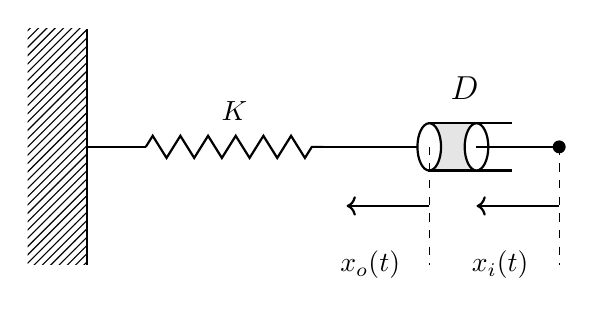
\begin{tikzpicture}[scale=1.5]
          % 固定壁
          \fill[pattern=north east lines] (-0.5,0) rectangle (0,2);
          \draw[thick] (0,0) -- (0,2);
        
          % バネ
          \draw[thick] (0,1) -- (0.5,1);
          \draw[thick, decorate, decoration={zigzag, segment length=10, amplitude=4}] (0.5,1) -- (2,1);
          \node at (1.25,1.3) {$K$};
        
          % --- ダンパー(シリンダー形) ---
    \draw[thick] (2,1) -- (2.9,1); % 棒(変更なし)
    \draw[thick, fill=gray!20] (2.9,0.8) rectangle (3.3,1.2); % 筒の側面
    \draw[thick] (3.3,1.2) -- (3.6,1.2);% 筒の側面(上)
    \draw[thick] (3.3,0.8) -- (3.6,0.8);% 筒の側面(下)
    \draw[thick, fill=white] (2.9,1) ellipse (0.1 and 0.2);   % 左側の端面(楕円)
    \draw[thick, fill=white] (3.3,1) ellipse (0.1 and 0.2);   % 右側の端面(楕円)
    \draw[thick] (3.3,1) -- (4.0,1); % ピストン棒 → 始点を 3.5 → 3.3 に変更
    \node at (3.2,1.5) {\large $D$};
    
    
          % 入力矢印
          \draw[->, thick] (4,0.5) -- (3.3,0.5);
          \node at (3.5,0) {$x_i(t)$};
        
          % 出力矢印
          \draw[->, thick] (2.9,0.5) -- (2.2,0.5);
          \node at (2.4,0) {$x_o(t)$};
        
          % 支点
          \draw[fill] (4,1) circle (0.05);
        
          % 点線
          \draw[dashed] (2.9,1) -- (2.9,0);
          \draw[dashed] (4.0,1) -- (4.0,0);
        \end{tikzpicture}
        \end{center}}]
    
    %解答

    \({x}_o(t),{x}_i(t)\)について運動方程式を立てると,
    \begin{align*}
        \left\{
            \begin{aligned}
                m_o \ddot{x}_o &= -K\,x_o - D\bigl(\dot{x}_o-\dot{x}_i\bigr),\\
                m_i \ddot{x}_i &= D\bigl(\dot{x}_o-\dot{x}_i\bigr) + f(t)
            \end{aligned}
        \right.
    \end{align*}
        ここで入力側にかかる力\(f(t)\)はわからないので,もう一方の式に着目すると,
    \begin{align*}
        &\qquad m_o \ddot{x}_o = -K\,x_o - D\bigl(\dot{x}_o-\dot{x}_i\bigr) \\
        &\therefore \quad m_o \ddot{x}_o + K\,x_o + D \dot{x}_o=D \dot{x}_i \\
        &\therefore \quad \mathcal{L} \left[  m_o \ddot{x}_o + D \dot{x}_o + K\,x_o  \right] 
        =\mathcal{L} \left[ D \dot{x}_i \right] \\
        &\therefore \quad (m_o s^2 + D s + K)\,X_o(s) = D\,s\,X_i(s). \quad [\because x_i(0)= 0, x_o(0)=0 ]\\
        &\therefore \quad G(s) \;=\;\frac{X_o(s)}{X_i(s)}
        \;=\;\frac{D\,s}{m_o s^2 + D s + K}\\
        &\therefore \quad G(s) = \frac{D\,s}{ D s + K} \quad [m_o=0 \text{とした} ]
    \end{align*}

\end{tcolorbox}
\newpage
% --------------- [30] --------------- 済
\begin{tcolorbox}[title={[30] 外力\(f(t)[N]\)を図の方向に考え,平衡点からの変位\(x(t)[m]\)を出力信号\\
    \qquad とみなしたときの伝達関数を求めよ. 
    \begin{center}
        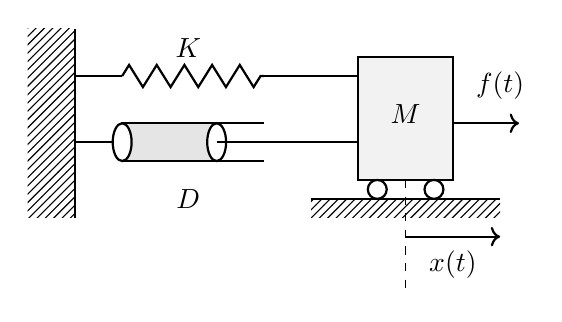
\begin{tikzpicture}[scale=1.2]
          % 固定壁
          \fill[pattern=north east lines] (-0.5,0) rectangle (0,2);
          \draw[thick] (0,0) -- (0,2);
        
          % バネ
          \draw[thick] (0,1.5) -- (0.5,1.5);
          \draw[thick, decorate, decoration={zigzag, segment length=10, amplitude=4}] (0.5,1.5) -- (2,1.5);
          \draw[thick] (2,1.5) -- (3.5,1.5);
          \node at (1.2,1.8) {$K$};
        
          % ダンパー(シリンダー形式)
          \draw[thick] (0,0.8) -- (0.5,0.8); % 棒
          \draw[thick, fill=gray!20] (0.5,0.6) rectangle (1.5,1.0); % 筒の側面
          \draw[thick] (1.5,1.0) -- (2,1.0); % 筒の上
          \draw[thick] (1.5,0.6) -- (2,0.6); % 筒の下
          \draw[thick, fill=white] (0.5,0.8) ellipse (0.1 and 0.2); % 左端面
          \draw[thick, fill=white] (1.5,0.8) ellipse (0.1 and 0.2); % 右端面
          \draw[thick] (1.5,0.8) -- (3,0.8); % ピストン棒
          \node at (1.2,0.2) {$D$};
        
          % 質量M
          \draw[thick, fill=gray!10] (3,0.4) rectangle (4,1.7);
          \node at (3.5,1.1) {$M$};
          % ローラー追加
            \draw[thick] (3.2,0.3) circle (0.1);
            \draw[thick] (3.8,0.3) circle (0.1);
    
        
          % 床
          \draw[thick] (2.5,0.2) -- (4.5,0.2);
          \fill[pattern=north east lines] (2.5,0) rectangle (4.5,0.2);
        
          % 座標
          \draw[->, thick] (3.5,-0.2) -- (4.5,-0.2);
          \node at (4,-0.5) {$x(t)$};
          \draw[dashed] (3.5,0.4) -- (3.5,-0.8);
        
          % 外力
          \draw[->, thick] (4,1) -- (4.7,1);
          \node at (4.5,1.4) {$f(t)$};
        \end{tikzpicture}
        \end{center}
        }]

        %解答

        \(x(t)\)に関する運動方程式より
        \begin{align*}
            &\qquad M\ddot{x} =f(t) -Kx - D \dot{x} \\
            &\therefore \quad M\ddot{x} + Kx + D \dot{x} =f(t) \\
            &\therefore \quad \mathcal{L} \left[ M\ddot{x} + D \dot{x} + Kx\right] 
            =\mathcal{L} \left[ f(t) \right] \\
            &\therefore \quad (M s^2 + D s + K)\,X(s) = F(s) \quad [\because x_i(0)= 0, x_o(0)=0 ]\\
            &\therefore \quad G(s) \;=\;\frac{X(s)}{F(s)}
            \;=\;\frac{1}{M s^2 + D s + K}
        \end{align*}

\end{tcolorbox}
% --------------- [31] --------------- 済
\begin{tcolorbox}[title={[31] 平衡点からの変位として,図中の\(x_i(t)[m]\)と\(x_o(t)[m]\)を考える.\\
    \qquad \(x_i(t)\)を入力信号,\(x_o(t)[m]\) を出力信号とみなしたときの伝達関数を求めよ.
    \begin{center}
        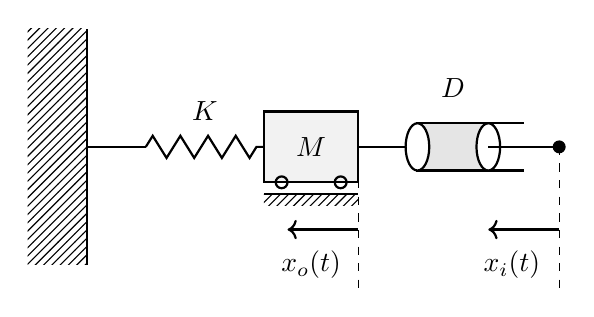
\begin{tikzpicture}[scale=1.5]
          % 固定壁
          \fill[pattern=north east lines] (-0.5,0) rectangle (0,2);
          \draw[thick] (0,0) -- (0,2);
    
          % バネ
          \draw[thick] (0,1) -- (0.5,1);
          \draw[thick, decorate, decoration={zigzag, segment length=10, amplitude=4}] (0.5,1) -- (1.5,1);
          \node at (1,1.3) {$K$};
        
          % 質量M
          \draw[thick, fill=gray!10] (1.5,0.7) rectangle (2.3,1.3);
          \node at (1.9,1) {$M$};
          % ローラー
          \draw[thick] (1.65,0.7) circle (0.05);
          \draw[thick] (2.15,0.7) circle (0.05);
          % 地面
          \draw[thick] (1.5,0.6) -- (2.3,0.6);
          \fill[pattern=north east lines] (1.5,0.5) rectangle (2.3,0.6);
        
          % ダンパー
          \draw[thick] (2.3,1) -- (2.8,1); % 棒
          \draw[thick, fill=gray!20] (2.8,0.8) rectangle (3.4,1.2); % 筒
          \draw[thick] (3.4,1.2) -- (3.7,1.2); % 筒上
          \draw[thick] (3.4,0.8) -- (3.7,0.8); % 筒下
          \draw[thick, fill=white] (2.8,1) ellipse (0.1 and 0.2);
          \draw[thick, fill=white] (3.4,1) ellipse (0.1 and 0.2);
          \draw[thick] (3.4,1) -- (4,1); % ピストン棒
          \node at (3.1,1.5) {$D$};
        
          % 入力矢印
          \draw[->, thick] (4,0.3) -- (3.4,0.3);
          \node at (3.6,0) {$x_i(t)$};
        
          % 出力矢印
          \draw[->, thick] (2.3,0.3) -- (1.7,0.3);
          \node at (1.9,0) {$x_o(t)$};
        
          % 支点
          \draw[fill] (4,1) circle (0.05);
        
          % 点線
          \draw[dashed] (2.3,1) -- (2.3,-0.2);
        \draw[dashed] (4,1) -- (4,-0.2);
        \end{tikzpicture}
        \end{center}
        }]

        \({x}_o(t),{x}_i(t)\)について運動方程式を立てると,
    \begin{align*}
        \left\{
            \begin{aligned}
                M\ddot{x}_o &= -K\,x_o - D\bigl(\dot{x}_o-\dot{x}_i\bigr),\\
                m\ddot{x}_i &= D\bigl(\dot{x}_o-\dot{x}_i\bigr) + f(t)
            \end{aligned}
        \right.
    \end{align*}
        ここで入力側にかかる力\(f(t)\)はわからないので,もう一方の式に着目すると,
    \begin{align*}
        &\qquad M\ddot{x}_o = -K\,x_o - D\bigl(\dot{x}_o-\dot{x}_i\bigr) \\
        &\therefore \quad M\ddot{x}_o + K\,x_o + D \dot{x}_o=D \dot{x}_i \\
        &\therefore \quad \mathcal{L} \left[  M\ddot{x}_o + D \dot{x}_o + K\,x_o  \right] 
        =\mathcal{L} \left[ D \dot{x}_i \right] \\
        &\therefore \quad (M s^2 + D s + K)\,X_o(s) = D\,s\,X_i(s). \quad [\because x_i(0)= 0, x_o(0)=0 ]\\
        &\therefore \quad G(s) \;=\;\frac{X_o(s)}{X_i(s)}
        \;=\;\frac{D\,s}{M s^2 + D s + K}
    \end{align*}


\end{tcolorbox}
% --------------- [32] --------------- 済
\begin{tcolorbox}[title={[32] 粘性減衰係数\(D_1[N \cdot s /m]\)のダッシュポットのピストンの平衡点からの変位\\
    \qquad \(x_i(t)[m]\)を入力信号,粘性減衰係数\(D_1[N \cdot s /m]\)のダッシュポットのピストン \\
    \qquad の平衡点からの   変位\(x_o(t)[m]\) を出力信号としたときの伝達関数を求めよ.
\begin{center}
  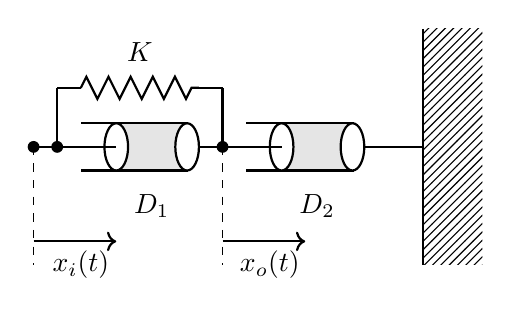
\begin{tikzpicture}[scale=1.5]
    % 固定壁
    \fill[pattern=north east lines] (4,0) rectangle (4.5,2);
    \draw[thick] (4,2) -- (4,0);
  
    % ダンパ D2
    \draw[thick, fill=gray!20] (2.8,0.8) rectangle (3.4,1.2);
    \draw[thick] (2.8,1.2) -- (2.5,1.2);
    \draw[thick] (2.8,0.8) -- (2.5,0.8);
    \draw[thick, fill=white] (2.8,1) ellipse (0.1 and 0.2);
    \draw[thick, fill=white] (3.4,1) ellipse (0.1 and 0.2);
    \draw[thick] (2,1) -- (2.8,1);
    \draw[thick] (3.5,1) -- (4,1);
    \node at (3.1,0.5) {$D_2$};
  
    % ダンパ D1
    \draw[thick, fill=gray!20] (1.4,0.8) rectangle (2.0,1.2);
    \draw[thick] (1.4,1.2) -- (1.1,1.2);
    \draw[thick] (1.4,0.8) -- (1.1,0.8);
    \draw[thick, fill=white] (1.4,1) ellipse (0.1 and 0.2);
    \draw[thick, fill=white] (2.0,1) ellipse (0.1 and 0.2);
    \draw[thick] (0.7,1) -- (1.4,1);
    \node at (1.7,0.5) {$D_1$};
  
    % バネ K
    \draw[thick] (0.9,1) -- (0.9,1.5);
    \draw[thick] (0.9,1.5) -- (1.1,1.5);
    \draw[thick, decorate, decoration={zigzag, segment length=8, amplitude=4}] (1.1,1.5) -- (2.1,1.5);
    \draw[thick] (2.1,1.5) -- (2.3,1.5);
    \draw[thick] (2.3,1) -- (2.3,1.5);
    \node at (1.6,1.8) {$K$};
  
    % 接点
    \fill (0.7,1) circle (0.05);
    \fill (0.9,1) circle (0.05);
    \fill (2.3,1) circle (0.05);

  
    % 点線(基準線)
    \draw[dashed] (0.7,1) -- (0.7,0);
    \draw[dashed] (2.3,1) -- (2.3,0);
  
    % 入力 x₁(t)
    \draw[->, thick] (0.7,0.2) -- (1.4,0.2);
    \node at (1.1,0) {$x_{i}(t)$};
  
    % 出力 x₂(t)
    \draw[->, thick] (2.3,0.2) -- (3,0.2);
    \node at (2.7,0) {$x_{o}(t)$};
    \end{tikzpicture}
    \end{center}}]

    \({x}_o(t),{x}_i(t)\)について運動方程式を立てると,
    \begin{align*}
        \left\{
            \begin{aligned}
                M\ddot{x}_i &= K(x_o - x_i) + D_1\bigl(\dot{x}_o-\dot{x}_i\bigr)+ f(t),\\
                m\ddot{x}_o &= - K(x_o - x_i) - D_1\bigl(\dot{x}_o-\dot{x}_i\bigr) - D_2 \dot{x}_o\\
            \end{aligned}
        \right.
    \end{align*}
        ここで入力側にかかる力\(f(t)\)はわからないので,もう一方の式に着目すると,
    \begin{align*}
        &\qquad m\ddot{x}_o = - K(x_o - x_i) - D_1\bigl(\dot{x}_o-\dot{x}_i\bigr) - D_2 \dot{x}_o \\
        &\therefore \quad m\ddot{x}_o + (D_1 +D_2) \dot{x}_o + K\,x_o = D_1 \dot{x}_i + K x_i\\
        &\therefore \quad \mathcal{L} \left[  m\ddot{x}_o + (D_1 +D_2) \dot{x}_o + K\,x_o  \right] 
        =\mathcal{L} \left[ D_1 \dot{x}_i + K x_i \right] \\
        &\therefore \quad \left\{m s^2 + (D_1+D_2) s + K\right\}\,X_o(s) 
        = (D_1s+K)X_i(s) \quad [\because x_i(0)= 0, x_o(0)=0 ]\\
        &\therefore \quad G(s) =\frac{X_o(s)}{X_i(s)}
        =\frac{D_1s+K}{m s^2 + (D_1+D_2) s + K}\\
        &\therefore \quad G(s) 
        = \frac{D_1s+K}{(D_1+D_2) s + K}\quad [\because m=0\text{とした}]
    \end{align*}

\end{tcolorbox}
\newpage
% --------------- [33] --------------- 済
\begin{tcolorbox}[title={[33] 平衡点からの変位として,図中の\(x_i(t)[m]\)と\(x_o(t)[m]\)を考える. \\
    \qquad \(x_i(t)[m]\)を入力信号,\(x_o(t)[m]\)を出力信号とみなしたときの伝達巻子を求めよ.\\
    \qquad 台車は摩擦なく床を動くものとする.すべての変数の初期値はゼロである.
    
    \begin{center}
        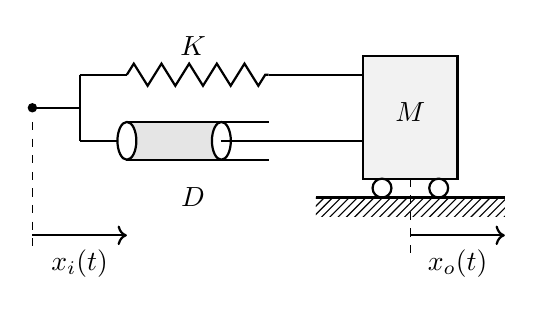
\begin{tikzpicture}[scale=1.2]
          % バネ
          \draw[thick] (0,1.5) -- (0.5,1.5);
          \draw[thick, decorate, decoration={zigzag, segment length=10, amplitude=4}] (0.5,1.5) -- (2,1.5);
          \draw[thick] (2,1.5) -- (3.5,1.5);
          \node at (1.2,1.8) {$K$};
        
          % ダンパー(シリンダー形式)
          \draw[thick] (0,0.8) -- (0.5,0.8); % 棒
          \draw[thick, fill=gray!20] (0.5,0.6) rectangle (1.5,1.0); % 筒の側面
          \draw[thick] (1.5,1.0) -- (2,1.0); % 筒の上
          \draw[thick] (1.5,0.6) -- (2,0.6); % 筒の下
          \draw[thick, fill=white] (0.5,0.8) ellipse (0.1 and 0.2); % 左端面
          \draw[thick, fill=white] (1.5,0.8) ellipse (0.1 and 0.2); % 右端面
          \draw[thick] (1.5,0.8) -- (3,0.8); % ピストン棒
          \node at (1.2,0.2) {$D$};
        
          % 質量M
          \draw[thick, fill=gray!10] (3,0.4) rectangle (4,1.7);
          \node at (3.5,1.1) {$M$};
          % ローラー追加
            \draw[thick] (3.2,0.3) circle (0.1);
            \draw[thick] (3.8,0.3) circle (0.1);
    
          % 床
          \draw[thick] (2.5,0.2) -- (4.5,0.2);
          \fill[pattern=north east lines] (2.5,0) rectangle (4.5,0.2);
        
          % 座標
          \draw[->, thick] (3.5,-0.2) -- (4.5,-0.2);
          \node at (4,-0.5) {$x_o(t)$};
          \draw[dashed] (3.5,0.4) -- (3.5,-0.4);
    
          \draw[->, thick] (-0.5,-0.2) -- (0.5,-0.2);
          \node at (0,-0.5) {$x_i(t)$};
          \draw[dashed] (-0.5,1) -- (-0.5,-0.4);
    
          \draw[thick] (0,0.8) -- (0,1.5);
          \draw[thick] (0,1.15) -- (-0.5,1.15);
    
          \fill (-0.5,1.15) circle (0.05);
    
        \end{tikzpicture}
        \end{center}}]
    
    \({x}_o(t),{x}_i(t)\)について運動方程式を立てると,
    \begin{align*}
        \left\{
            \begin{aligned}
                m\ddot{x}_i &= K(x_o - x_i) + D\bigl(\dot{x}_o-\dot{x}_i\bigr)+ f(t),\\
                M\ddot{x}_o &= - K(x_o - x_i) - D\bigl(\dot{x}_o-\dot{x}_i\bigr) \\
            \end{aligned}
        \right.
    \end{align*}
        ここで入力側にかかる力\(f(t)\)はわからないので,もう一方の式に着目すると,
    \begin{align*}
        &\qquad M\ddot{x}_o = - K(x_o - x_i) - D\bigl(\dot{x}_o-\dot{x}_i\bigr)  \\
        &\therefore \quad M\ddot{x}_o + D\dot{x}_o + K\,x_o = D_1 \dot{x}_i + K x_i\\
        &\therefore \quad \mathcal{L} \left[  M\ddot{x}_o + D \dot{x}_o + K\,x_o  \right] 
        =\mathcal{L} \left[ D \dot{x}_i + K x_i \right] \\
        &\therefore \quad \left\{M s^2 + D s + K\right\}\,X_o(s) 
        = (Ds+K)X_i(s) \quad [\because x_i(0)= 0, x_o(0)=0 ]\\
        &\therefore \quad G(s) \;=\;\frac{X_o(s)}{X_i(s)}
        \;=\;\frac{Ds+K}{M s^2 + Ds + K}
    \end{align*}

\end{tcolorbox}
% --------------- [34] ---------------  済
\begin{tcolorbox}[title={[34]この系の伝達関数を求めよ.ただし,fは粘性抵抗係数であり,\\
    \qquad 初期条件\(t = 0\)において\(F=0\)
    \begin{center}
        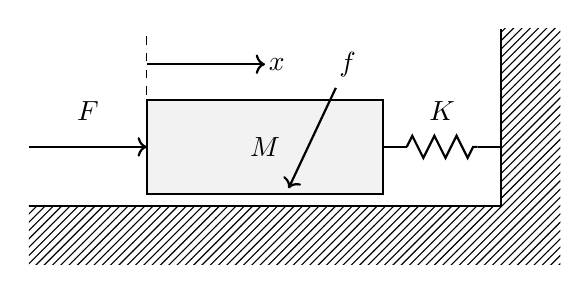
\begin{tikzpicture}[scale=1.5]
          % 固定壁
          \draw[thick] (4,2) -- (4,0.5);
          \fill[pattern=north east lines] (4,0) rectangle (4.5,2);
        
          % バネ
          \draw[thick] (3,1) -- (3.2,1);
          \draw[thick, decorate, decoration={zigzag, segment length=8, amplitude=4}] (3.2,1) -- (3.8,1);
          \draw[thick] (3.8,1) -- (4,1);
          \node at (3.5,1.3) {$K$};
        
          % 質量M
          \draw[thick, fill=gray!10] (1,0.6) rectangle (3,1.4);
          \node at (2,1) {$M$};
    
          %粘性抵抗係数
          \draw[->, thick] (2.6,1.5) -- (2.2,0.65);
          \node at (2.7,1.7) {$f$};
    
          % 地面
          \draw[thick] (0,0.5) -- (4,0.5);
          \fill[pattern=north east lines] (0,0) rectangle (4,0.5);
        
          % 外力
          \draw[->, thick] (0,1) -- (1,1);
          \node at (0.5,1.3) {$F$};
        
          % 点線
          \draw[dashed] (1,0.6) -- (1,2);
        
          % 座標
          \draw[->, thick] (1,1.7) -- (2,1.7);
          \node at (2.1,1.7) {$x$};
        \end{tikzpicture}
        \end{center}}]

        \({x}(t)\)について運動方程式を立てると,
    \begin{align*}
        & \qquad M\ddot{x} = -Kx+ - f\dot{x} + F(t) \\
        &\therefore \quad M\ddot{x} + f\dot{x} + Kx = F(t)\\
        &\therefore \quad \mathcal{L} \left[  M\ddot{x} + f\dot{x} + Kx \right] 
        =\mathcal{L} \left[ F(t) \right] \\
        &\therefore \quad \left\{M s^2 + f s + K\right\}\,X(s) 
        = F(s) \quad [\because x(0)= 0, x(0)=0 ]\\
        &\therefore \quad G(s) = \frac{X(s)}{F(s)}
        = \frac{1}{M s^2 + f s + K}
    \end{align*}

\end{tcolorbox}
% --------------- [35] --------------- 済
\begin{tcolorbox}[title={[35] 長さ\(y_0\)のばねの上端を固定し,下端に質量\(M\)の物体をつり下げたとき,\\
    \qquad ばねの長さが\(y_1\)になって平衡した.\\
    \qquad つぎに,物体に下向きの力\(F(t)\) を加えたとき,物体の平衡状態からの変位を\\
    \qquad \(y\)として運動方程式を作れ.\\
    \qquad ただし物体と側壁との間には,粘性摩擦定数を\(f\)とする.

    \begin{center}
        \begin{tikzpicture}[scale=1.2]
        % 左側(平衡状態)
        \node at (-2,-1)[scale=0.6] {$質量-ばね-まさつ系(平衡状態)$};
    
            %壁
            \draw[thick] (-3,0) -- (-3,4);
            \draw[thick] (-3,4) -- (-1,4);
            \draw[thick] (-1,0) -- (-1,4);
            \fill[pattern=north east lines] (-3.5,0) rectangle (-3,4);
            \fill[pattern=north east lines] (-3.5,4) rectangle (-0.5,4.5);
            \fill[pattern=north east lines] (-1,0) rectangle (-0.5,4);
    
    
            %ばね
            \draw[thick] (-2,1) -- (-2,2);
            \draw[thick, decorate, decoration={coil, segment length=6}] (-2,2) -- (-2,3);
            \draw[thick] (-2,3) -- (-2,4);
            \node at (-2.3,2.5) {$K$};
    
            %重り
            \draw[thick, fill=gray!10] (-2.9,0.2) rectangle (-1.1,1);
            \node at (-2,0.6) {$M$};
    
            %粘性摩擦定数
            \draw[->, thick] (-1.3,0) -- (-1.1,0.6);
            \node at (-1.4,-0.2) {$f$};
    
            %重り
            \draw[dashed] (-2.9,1.2) rectangle (-1.1,2);
    
            %座標
            \draw[dashed] (-4.5,4) -- (-3,4);
            \draw[dashed] (-4.5,1) -- (-2.9,1);
            \draw[dashed] (-4,2) -- (-2.9,2);
    
            \draw[<->,thick] (-3.8,4) -- (-3.8,2);
            \node at (-3.95,3) {$y_0$};
            \draw[<->,thick] (-4.3,4) -- (-4.3,1);
            \node at (-4.45,2.5) {$y_1$};
          
          % 左側(平衡状態)
          \node at (2,-1)[scale=0.6] {$力を加えた場合$};
    
            %壁
            \draw[thick] (3,0) -- (3,4);
            \draw[thick] (3,4) -- (1,4);
            \draw[thick] (1,0) -- (1,4);
            \fill[pattern=north east lines] (3.5,0) rectangle (3,4);
            \fill[pattern=north east lines] (3.5,4) rectangle (0.5,4.5);
            \fill[pattern=north east lines] (1,0) rectangle (0.5,4);
    
    
            %ばね
            \draw[thick] (2,1.3) -- (2,2.2);
            \draw[thick, decorate, decoration={coil, segment length=6}] (2,2.2) -- (2,3.1);
            \draw[thick] (2,3.1) -- (2,4);
            \node at (2.3,2.65) {$K$};
    
            %重り
            \draw[thick, fill=gray!10] (2.9,0.5) rectangle (1.1,1.3);
            \node at (2,0.9) {$M$};
    
            %粘性摩擦定数
            \draw[->, thick] (2.7,0) -- (2.9,0.6);
            \node at (2.6,-0.2) {$f$};
    
            %座標
            \draw[dashed] (0.1,4) -- (1,4);
            \draw[dashed] (0.1,1.3) -- (1.1,1.3);
            \draw[dashed] (2.9,1.3) -- (4,1.3);
    
            \draw[<->,thick] (0.3,4) -- (0.3,1.3);
            \node at (0,2.65) {$y_1$};
    
            \draw[->,thick] (3.8,1.3) -- (3.8,0.5);
            \node at (3.8,0.3) {$y$};
    
            
        
        \end{tikzpicture}
        \end{center}
        }]

        \({y}(t)\)について運動方程式を立てると,
        \begin{align*}
            & \qquad M\ddot{y} = F(t) - f\dot{y} - Ky 
        \end{align*}

\end{tcolorbox}
% --------------- [36] --------------- 済
\begin{tcolorbox}[title={[36] 質量\(M\)の物体の一端にばねをつけ,\\
    \qquad ばねを力\(F\)で引っ張ったときの運動方程式を作れ.  \\
    \qquad 物体と床面との間の粘性摩擦定数を\(f\)とする.
    
    \begin{center}
        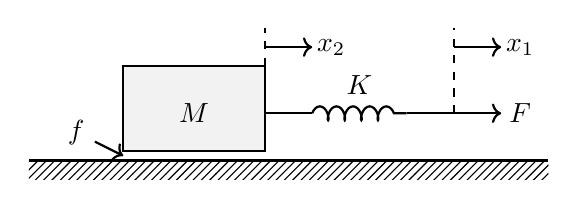
\begin{tikzpicture}[scale=1.2]
          % 地面
          \draw[thick] (-0.5,0) -- (5,0);
          \fill[pattern=north east lines] (-0.5,-0.2) rectangle (5,0);
        
          % 質量M
          \draw[thick, fill=gray!10] (0.5,0.1) rectangle (2,1);
          \node at (1.25,0.5) {$M$};
          \draw[dashed] (2,1.0) -- (2,1.4);
        
          % 摩擦f
          \draw[->,thick] (0.2,0.2) -- (0.5,0.05);
          \node at (0,0.3) {$f$};
        
          % バネ
          \draw[thick] (2,0.5) -- (2.5,0.5);
          \draw[thick, decorate, decoration={coil, segment length=6}] (2.5,0.5) -- (3.5,0.5);
          \node at (3,0.8) {$K$};
          \draw[dashed] (4,0.5) -- (4,1.4);
        
          % 外力
          \draw[->, thick] (3.5,0.5) -- (4.5,0.5);
          \node at (4.7,0.5) {$F$};
        
          % 座標 x2
          \draw[->, thick] (2,1.2) -- (2.5,1.2);
          \node at (2.7,1.2) {$x_2$};
        
          % 座標 x1
          \draw[->, thick] (4,1.2) -- (4.5,1.2);
          \node at (4.7,1.2) {$x_1$};
        \end{tikzpicture}
        \end{center}
        }]

        \({x}_1(t),{x}_2(t)\)について運動方程式を立てると,
    \begin{align*}
        \left\{
            \begin{aligned}
                m\ddot{x}_1 &= -K(x_1 - x_2) + F(t),\\
                M\ddot{x}_2 &=  K(x_1 - x_2) - f \dot{x}_2 \\
            \end{aligned}
        \right.
    \end{align*}
        ここで\(m=0\)として二式を合わせると
    \begin{align*}
        &\qquad M\ddot{x}_2 = F(t)- f \dot{x}_2  
    \end{align*}

\end{tcolorbox}
\newpage
% --------------- [37] --------------- 済
\begin{tcolorbox}[title={[37] 等価変換によってひとつのブロックに簡単化せよ.
    \begin{center}
        
    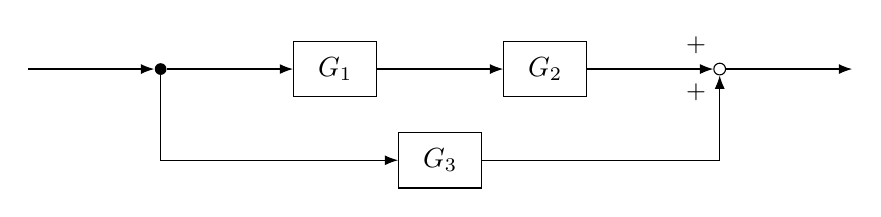
\begin{tikzpicture}[auto, node distance=1.2cm and 1.6cm, >=Latex]
  
        % --- ノード定義 ---
        \node[input] (input) {};
        \node[circle, fill=black, inner sep=1.5pt, right=of input] (branch) {};     % 分岐点
        \node[block, right=of branch] (G1) {$G_1$};
        \node[block, right=of G1] (G2) {$G_2$};
        \node[circle, draw, inner sep=1.5pt, right=of G2] (sum) {};                % 合流点
        \node[output, right=of sum] (output) {};
  
        \node[block, below=0.8cm of $(G1)!0.5!(G2)$] (G3) {$G_3$};                 % G3(下)
  
        % --- 線描画 ---
        \draw[->] (input) -- (branch);
        \draw[->] (branch) -- (G1);
        \draw[->] (G1) -- (G2);
        \draw[->] (G2) -- (sum);
        \draw[->] (sum) -- (output);
  
        \draw[->] (branch) |- (G3);
        \draw[->] (G3) -| (sum);
  
        % --- 加算記号 ---
        \node at ($(sum)+(-0.3,0.3)$) {\small $+$};
        \node at ($(sum)+(-0.3,-0.3)$) {\small $+$};
  
    \end{tikzpicture}
  
  
    \end{center}
    }]
    % --- Step 1:G1, G2 を合成して G1G2 ---
    \begin{center}
    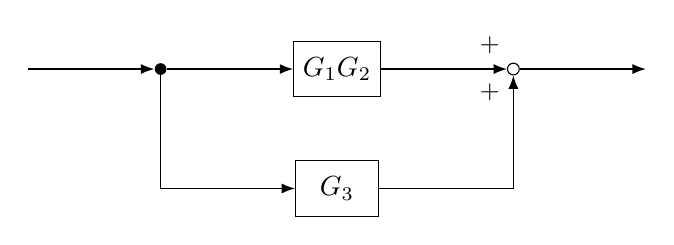
\begin{tikzpicture}[auto, node distance=1.2cm and 1.6cm, >=Latex]
  
      \node[input] (input) {};
      \node[circle, fill=black, inner sep=1.5pt, right=of input] (branch) {};
      \node[block, right=of branch] (G1G2) {$G_1 G_2$};
      \node[circle, draw, inner sep=1.5pt, right=of G1G2] (sum) {};
      \node[output, right=of sum] (output) {};
    
      \node[block, below=0.8cm of G1G2] (G3) {$G_3$};
    
      \draw[->] (input) -- (branch);
      \draw[->] (branch) -- (G1G2);
      \draw[->] (G1G2) -- (sum);
      \draw[->] (sum) -- (output);
    
      \draw[->] (branch) |- (G3);
      \draw[->] (G3) -| (sum);
    
      \node at ($(sum)+(-0.3,0.3)$) {\small $+$};
      \node at ($(sum)+(-0.3,-0.3)$) {\small $+$};
    
    \end{tikzpicture}
    \vspace{2mm}
    
    % --- 大きな下向き矢印(TikZで描画) ---
  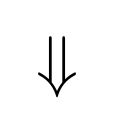
\begin{tikzpicture}
    \node (arrow) {\Huge$\Downarrow$};
  \end{tikzpicture}
  \vspace{2mm}
  
    % --- Step 2:G1G2 + G3 に合成 ---
    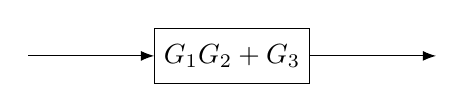
\begin{tikzpicture}[auto, node distance=1.2cm and 1.6cm, >=Latex]
  
      \node[input] (input) {};
      \node[block, right=of input] (Gtotal) {$G_1 G_2 + G_3$};
      \node[output, right=of Gtotal] (output) {};
    
      \draw[->] (input) -- (Gtotal);
      \draw[->] (Gtotal) -- (output);
    
    \end{tikzpicture}
  \end{center}
  
\end{tcolorbox}
% --------------- [38] --------------- 済
\begin{tcolorbox}[title={[38] 等価変換によってひとつのブロックに簡単化せよ. 
    \begin{center}
  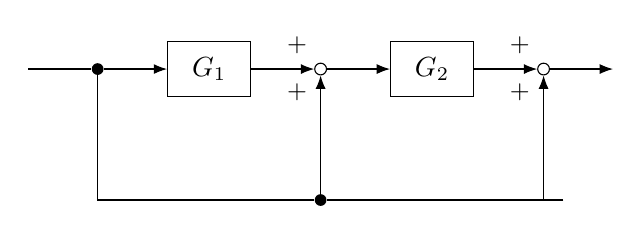
\begin{tikzpicture}[auto, node distance=1.2cm and 0.8cm, >=Latex]
  
    % ノード定義
    \node[input] (input) {};
    \node[circle, fill=black, inner sep=1.5pt, minimum size=3pt, right=of input] (branch) {}; % 分岐点:黒丸(サイズ修正)
  
    \node[block, right=of branch] (G1) {$G_1$};
    \node[circle, draw, inner sep=1.5pt, minimum size=3pt, right=of G1] (sum1) {}; % 中間合流点:白丸
  
    \node[block, right=of sum1] (G2) {$G_2$};
    \node[circle, draw, inner sep=1.5pt, minimum size=3pt, right=of G2] (sum2) {}; % 出力直前合流点:白丸
  
    \node[output, right=of sum2] (output) {};
  
    \node[circle, fill=black, inner sep=1.5pt, minimum size=3pt, below=1.5cm of sum1] (branch2) {}; % 下の黒丸(サイズ修正)
    
  
    % 線描画
    \draw[-] (input) -- (branch);
    \draw[->] (branch) -- (G1);
    \draw[->] (G1) -- (sum1);
    \draw[->] (sum1) -- (G2);
    \draw[->] (G2) -- (sum2);
    \draw[->] (sum2) -- (output);
  
    \draw[-] (branch) |- (branch2);
    \draw[->] (branch2.north) -| (sum1);
  
    \draw[-] (branch2.east) -- ++(3.0,0); % .east を使うと右側から出る
    \draw[->] ($(branch2.east)+(3.0,0)$) - | (sum2);
    
    % 加算記号を合流点にそれぞれ配置
    \node at ($(sum1)+(-0.3,0.3)$) {\small $+$};
    \node at ($(sum1)+(-0.3,-0.3)$) {\small $+$};
  
    \node at ($(sum2)+(-0.3,0.3)$) {\small $+$};
    \node at ($(sum2)+(-0.3,-0.3)$) {\small $+$};
  
  \end{tikzpicture}
    \end{center}
    \vspace{2mm}
    }]
    
    \begin{center}
  
      % --- Step 1:分岐1→分岐2→G1→合流1→G2→合流2、かつ2本の分岐線が交差しない構造 ---
      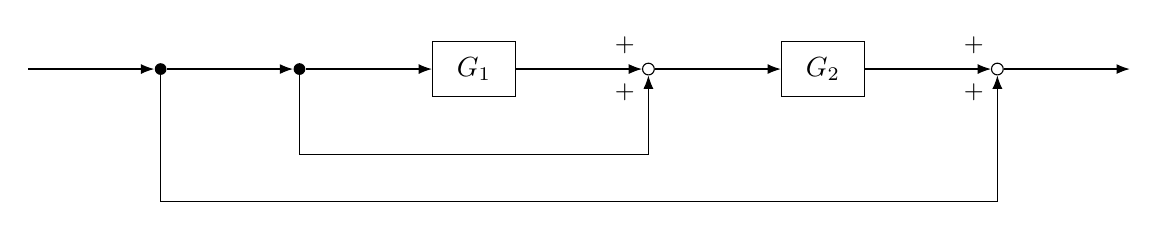
\begin{tikzpicture}[auto, node distance=1.2cm and 1.6cm, >=Latex]
      
        % 上部構造
        \node[input] (input) {};
        \node[circle, fill=black, inner sep=1.5pt, right=of input] (branch1) {}; % 分岐①
        \node[circle, fill=black, inner sep=1.5pt, right=of branch1] (branch2) {}; % 分岐②
        \node[block, right=of branch2] (G1) {$G_1$};
        \node[circle, draw, inner sep=1.5pt, right=of G1] (sum1) {}; % 合流①
        \node[block, right=of sum1] (G2) {$G_2$};
        \node[circle, draw, inner sep=1.5pt, right=of G2] (sum2) {}; % 合流②
        \node[output, right=of sum2] (output) {};
      
        % フィード線(分岐② → 合流①)
        \coordinate (feed1start) at (branch2.south);
        \coordinate (feed1end) at (sum1.south);
        \draw[->] (feed1start) |- ++(0,-1.0) -| (feed1end);
      
        % フィード線(分岐① → 合流②)
        \coordinate (feed2start) at (branch1.south);
        \coordinate (feed2end) at (sum2.south);
        \draw[->] (feed2start) |- ++(0,-1.6) -| (feed2end);
      
        % 上部のメインライン
        \draw[->] (input) -- (branch1);
        \draw[->] (branch1) -- (branch2);
        \draw[->] (branch2) -- (G1);
        \draw[->] (G1) -- (sum1);
        \draw[->] (sum1) -- (G2);
        \draw[->] (G2) -- (sum2);
        \draw[->] (sum2) -- (output);
      
        % 加算記号
        \node at ($(sum1)+(-0.3,0.3)$) {\small $+$};
        \node at ($(sum1)+(-0.3,-0.3)$) {\small $+$};
        \node at ($(sum2)+(-0.3,0.3)$) {\small $+$};
        \node at ($(sum2)+(-0.3,-0.3)$) {\small $+$};
      
      \end{tikzpicture}
      
      % --- 大きな下向き矢印(TikZで描画) ---
    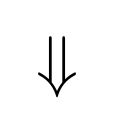
\begin{tikzpicture}
      \node (arrow) {\Huge$\Downarrow$};
    \end{tikzpicture}
    \vspace{2mm}
  
      % --- Step 2:G1 + 1 → G2 の直列化、もう1本はそのまま合流 ---
      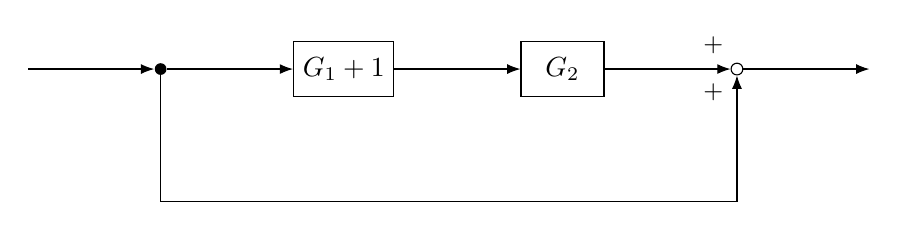
\begin{tikzpicture}[auto, node distance=1.2cm and 1.6cm, >=Latex]
      
        \node[input] (input) {};
        \node[circle, fill=black, inner sep=1.5pt, right=of input] (branch1) {}; % 分岐①
        \node[block, right=of branch1] (G1plus1) {$G_1 + 1$};
        \node[block, right=of G1plus1] (G2) {$G_2$};
        \node[circle, draw, inner sep=1.5pt, right=of G2] (sum) {}; % 合流②
        \node[output, right=of sum] (output) {};
      
        % 残る1本のルート(分岐① → 合流②)
        \coordinate (feedstart) at (branch1.south);
        \coordinate (feedend) at (sum.south);
        \draw[->] (feedstart) |- ++(0,-1.6) -| (feedend);
      
        % 上部のメインライン
        \draw[->] (input) -- (branch1);
        \draw[->] (branch1) -- (G1plus1);
        \draw[->] (G1plus1) -- (G2);
        \draw[->] (G2) -- (sum);
        \draw[->] (sum) -- (output);
      
        % 加算記号
        \node at ($(sum)+(-0.3,0.3)$) {\small $+$};
        \node at ($(sum)+(-0.3,-0.3)$) {\small $+$};
      \end{tikzpicture}
      
      % --- 大きな下向き矢印(TikZで描画) ---
    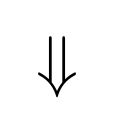
\begin{tikzpicture}
      \node (arrow) {\Huge$\Downarrow$};
    \end{tikzpicture}
    \vspace{2mm}
  
      % --- Step 3:最終形 (G1 + 1)G2 + 1 ---
      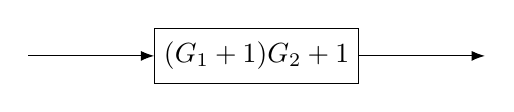
\begin{tikzpicture}[auto, node distance=1.2cm and 1.6cm, >=Latex]
      
        \node[input] (input) {};
        \node[block, right=of input] (Gtotal) {$(G_1 + 1)G_2 + 1$};
        \node[output, right=of Gtotal] (output) {};
      
        \draw[->] (input) -- (Gtotal);
        \draw[->] (Gtotal) -- (output);
      
      \end{tikzpicture}
      
      
  
  
      \end{center}
      
  
  \end{tcolorbox}
% --------------- [39] --------------- 済
\begin{tcolorbox}[title={[39] 等価変換によってひとつのブロックに簡単化せよ. 
    \begin{center}
  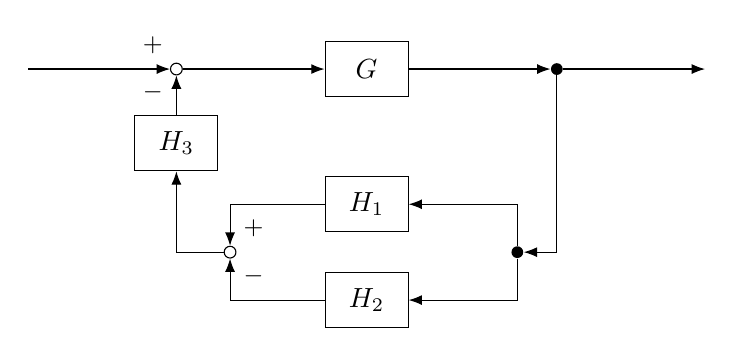
\begin{tikzpicture}[auto, node distance=1.0cm and 1.8cm, >=Latex]
  
    % --- 上段ノード ---
    \node[input] (input) {};
    \node[circle, draw, inner sep=1.5pt, right=of input] (sum1) {};              % 合流点①
    \node[block, right=of sum1] (G) {$G$};                                       % G
    \node[circle, fill=black, inner sep=1.5pt, right=of G] (branch1) {};         % 分岐点①
    \node[output, right=of branch1] (output) {};                                 % 出力
  
    % --- H₁・H₂ 縦並び(Gの真下) ---
    \node[block, below=1.0cm of G] (H1) {$H_1$};
    \node[block, below=0.5cm of H1] (H2) {$H_2$};
    \coordinate (midH) at ($(H1)!0.5!(H2)$);
  
    % --- 分岐点②(右):H₁とH₂の中間、高さmidH、X位置はGとbranch1の中間よりやや右
    \path (G) -- (branch1) coordinate[pos=0.6] (betweenGB);
    \node[circle, fill=black, inner sep=1.5pt] at ($(midH)+(betweenGB)-(G)+(0.3,0)$) (branch2) {}; % 分岐点②
  
    % --- 合流点②(左):midH高さ、X位置はHₛとGの中間
    \node[block, below=0.5cm of sum1] (Hs) {$H_3$};                              % H_s
    \path (sum1) -- (G) coordinate[pos=0.5] (leftX);
    \node[circle, draw, inner sep=1.5pt] at ($(midH)+(leftX)-(G)+(-0.3,0)$) (sum2) {};  % 合流点②
  
    % === 経路 ===
    \draw[->] (input) -- (sum1);
    \draw[->] (sum1) -- (G);
    \draw[->] (G) -- (branch1);
    \draw[->] (branch1) -- (output);
  
    \draw[->] (branch1) |- (branch2);                 % 分岐1 → 分岐2
    \draw[->] (branch2) |- (H1);                      % 分岐2 → H1(上方向)
    \draw[->] (branch2) |- (H2);                      % 分岐2 → H2(下方向)
  
    \draw[->] (H1) -| (sum2);                         % H1 → 合流2
    \draw[->] (H2) -| (sum2);                         % H2 → 合流2
  
    \draw[->] (sum2) -| (Hs);                         % 合流2 → Hs
    \draw[->] (Hs) -- (sum1);                         % Hs → 合流1(フィードバック)
  
    % --- 加算記号(揃え済) ---
    \node at ($(sum1)+(-0.3,0.3)$) {\small $+$};
    \node at ($(sum1)+(-0.3,-0.3)$) {\small $-$};
    \node at ($(sum2)+(0.3,0.3)$) {\small $+$};
    \node at ($(sum2)+(0.3,-0.3)$) {\small $-$};
  
  \end{tikzpicture}
    \end{center}
    }]
  
    \begin{center}
  
      % --- Step 1:H₁ - H₂ に合成 ---
        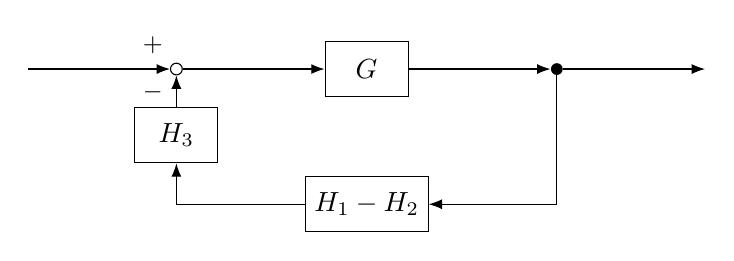
\begin{tikzpicture}[auto, node distance=1.0cm and 1.8cm, >=Latex]
        
          % メインライン
          \node[input] (input) {};
          \node[circle, draw, inner sep=1.5pt, right=of input] (sum1) {};
          \node[block, right=of sum1] (G) {$G$};
          \node[circle, fill=black, inner sep=1.5pt, right=of G] (branch1) {};
          \node[output, right=of branch1] (output) {};
        
          % フィードバック合成ブロック
          \node[block, below=1.0cm of G] (H1minusH2) {$H_1 - H_2$};
          \node[block, below=0.4cmof sum1] (Hs) {$H_3$};
        
          % 線
          \draw[->] (input) -- (sum1);
          \draw[->] (sum1) -- (G);
          \draw[->] (G) -- (branch1);
          \draw[->] (branch1) -- (output);
        
          \draw[->] (branch1) |- (H1minusH2);
          \draw[->] (H1minusH2) -|(Hs);
          \draw[->] (Hs) -- (sum1);
        
          % 符号
          \node at ($(sum1)+(-0.3,0.3)$) {\small $+$};
          \node at ($(sum1)+(-0.3,-0.3)$) {\small $-$};
        
        \end{tikzpicture}
  
      
      \vspace{1.2em}
      
      % --- 下向き矢印 ---
      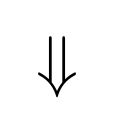
\begin{tikzpicture}
        \node {\Huge$\Downarrow$};
      \end{tikzpicture}
      
      \vspace{1.2em}
      
      % --- Step 2:Hₛ(H₁ - H₂) に直列合成し、負帰還構造に ---
      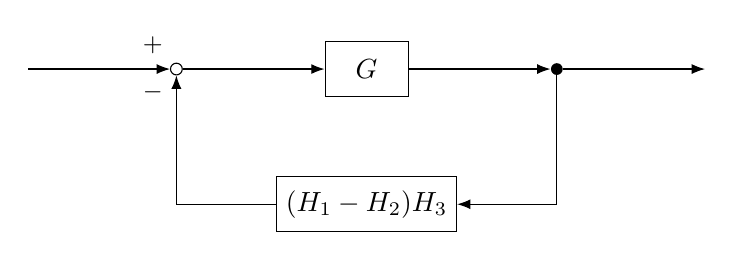
\begin{tikzpicture}[auto, node distance=1.0cm and 1.8cm, >=Latex]
      
        \node[input] (input) {};
        \node[circle, draw, inner sep=1.5pt, right=of input] (sum) {};
        \node[block, right=of sum] (G) {$G$};
        \node[circle, fill=black, inner sep=1.5pt, right=of G] (branch) {};
        \node[output, right=of branch] (output) {};
      
        \node[block, below=1.0cm of G] (Hfb) {$(H_1 - H_2)H_3$};
      
        \draw[->] (input) -- (sum);
        \draw[->] (sum) -- (G);
        \draw[->] (G) -- (branch);
        \draw[->] (branch) -- (output);
      
        \draw[->] (branch) |- (Hfb);
        \draw[->] (Hfb) -| (sum);
      
        \node at ($(sum)+(-0.3,0.3)$) {\small $+$};
        \node at ($(sum)+(-0.3,-0.3)$) {\small $-$};
      
      \end{tikzpicture}
      
      \vspace{1.2em}
      
      % --- 下向き矢印 ---
      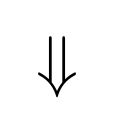
\begin{tikzpicture}
        \node {\Huge$\Downarrow$};
      \end{tikzpicture}
      
      \vspace{1.2em}
      
      % --- Step 3:最終形 G / (1 + G Hₛ(H₁ - H₂)) ---
      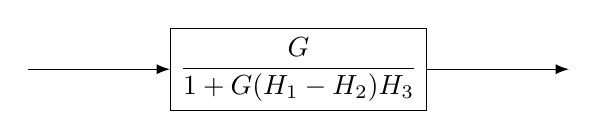
\begin{tikzpicture}[auto, node distance=1.0cm and 1.8cm, >=Latex]
      
        \node[input] (input) {};
        \node[block, right=of input] (total) {$\dfrac{G}{1 + G (H_1 - H_2)H_3}$};
        \node[output, right=of total] (output) {};
      
        \draw[->] (input) -- (total);
        \draw[->] (total) -- (output);
      
      \end{tikzpicture}
      
      \end{center}
      
  \end{tcolorbox}
% --------------- [40] --------------- 済
\begin{tcolorbox}[title={[40] 等価変換によってひとつのブロックに簡単化せよ.
  \begin{center}
\begin{tikzpicture}[auto, node distance=0.8cm and 0.8cm, >=Latex]

  % --- 上段ノード(左→右) ---
  \node[block] (G2) {$G_2$};
  \node[circle, fill=black, inner sep=1.5pt, right=of G2] (branch1) {};     % 分岐点①
  \node[circle, draw, inner sep=1.5pt, right=of branch1] (sum1) {};         % 合流点①
  \node[block, right=of sum1] (G1) {$G_1$};                                 % G_1
  \node[circle, fill=black, inner sep=1.5pt, right=of G1] (branch2) {};     % 分岐点②
  \node[output, right=of branch2] (output) {};                              % 出力

  % --- 下段ノード ---
  \node[circle, draw, inner sep=1.5pt, below=1.5cm of branch1] (sum2) {};   % 合流点②
  \node[input, above=1.8cm of sum1] (input) {};                             % 入力(合流点①の上)

  % === 経路 ===
  \draw[->] (input) -- (sum1);                       % input ↓ 合流点1
  \draw[->] (sum1) -- (G1);                          % 合流点1 → G1
  \draw[->] (G1) -- (branch2);                       % G1 → 分岐点2
  \draw[->] (branch2) -- (output);                   % 分岐点2 → 出力

  \draw[->] (branch2) |- (sum2);                     % 分岐点2 → 合流点2(下)

  \draw[->] (sum2) -| ($(G2.west)+(-0.8,0)$) -- (G2); % ←↑→経路:合流点2 → 左 → 上 → G2

  \draw[->] (G2) -- (branch1);                       % G2 → 分岐点1
  \draw[->] (branch1) -- (sum1);                     % 分岐点1 → 合流点1
  \draw[->] (branch1) -- (sum2);                     % 分岐点1 → 合流点2(短絡)

  % --- 加算記号配置 ---
  \node at ($(sum1)+(-0.3,0.3)$) {\small $+$};
  \node at ($(sum1)+(-0.3,-0.3)$) {\small $+$};
  \node at ($(sum2)+(0.3,0.3)$) {\small $+$};
  \node at ($(sum2)+(0.3,-0.3)$) {\small $+$};

\end{tikzpicture}
  \end{center}
  }]    

  \begin{center}

    % --- Step 1:G₂を含む簡約前の構造(オリジナル) ---
    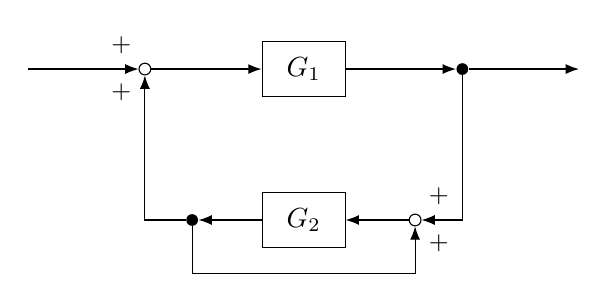
\begin{tikzpicture}[auto, node distance=1.0cm and 1.4cm, >=Latex]
    
      \node[input] (input) {};
      \node[circle, draw, inner sep=1.5pt, right=of input] (sum1) {};
      \node[block, right=of sum1] (G1) {$G_1$};
      \node[circle, fill=black, inner sep=1.5pt, right=of G1] (branch2) {};
      \node[output, right=of branch2] (output) {};
    
      \node[block, below=1.2cm of G1] (G2) {$G_2$};
      \node[circle, draw, inner sep=1.5pt, right=0.8cm of G2] (sum2) {};
      \node[circle, fill=black, inner sep=1.5pt, left=0.8cm of G2] (branch1) {};
    
      \draw[->] (input) -- (sum1);
      \draw[->] (sum1) -- (G1);
      \draw[->] (G1) -- (branch2);
      \draw[->] (branch2) -- (output);
    
      \draw[->] (branch2) |- (sum2);
      \draw[->] (sum2) -- (G2);
      \draw[->] (G2) -- (branch1);
      \draw[->] (branch1) -| (sum1);
      
      \coordinate (feed2start) at (branch1.south);
        \coordinate (feed2end) at (sum2.south);
        \draw[->] (feed2start) |- ++(0,-0.6) -| (feed2end);
    
      \node at ($(sum1)+(-0.3,0.3)$) {\small $+$};
      \node at ($(sum1)+(-0.3,-0.3)$) {\small $+$};
      \node at ($(sum2)+(0.3,0.3)$) {\small $+$};
      \node at ($(sum2)+(0.3,-0.3)$) {\small $+$};
    
    \end{tikzpicture}
    
    \vspace{1.2em}
    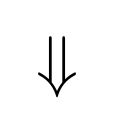
\begin{tikzpicture}
      \node {\Huge$\Downarrow$};
    \end{tikzpicture}
    \vspace{1.2em}
    
    % --- Step 2:G₂部分を簡約して G₂/(1-G₂) に置換 ---
    \begin{tikzpicture}[auto, node distance=1.0cm and 1.6cm, >=Latex]
    
      \node[input] (input) {};
      \node[circle, draw, inner sep=1.5pt, right=of input] (sum1) {};
      \node[block, right=of sum1] (G1) {$G_1$};
      \node[circle, fill=black, inner sep=1.5pt, right=of G1] (branch) {};
      \node[output, right=of branch] (output) {};
    
      \node[block, below=1.2cm of G1] (G2loop) {$\dfrac{G_2}{1 - G_2}$};
    
      \draw[->] (input) -- (sum1);
      \draw[->] (sum1) -- (G1);
      \draw[->] (G1) -- (branch);
      \draw[->] (branch) -- (output);
    
      \draw[->] (branch) |- (G2loop);
      \draw[->] (G2loop) -| (sum1);
    
      \node at ($(sum1)+(-0.3,0.3)$) {\small $+$};
      \node at ($(sum1)+(-0.3,-0.3)$) {\small $+$};
    
    \end{tikzpicture}
    
    \vspace{1.2em}
    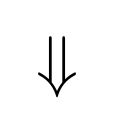
\begin{tikzpicture}
      \node {\Huge$\Downarrow$};
    \end{tikzpicture}
    \vspace{1.2em}
    
    % --- Step 3:全体を1つのブロックへ簡約1 ---
    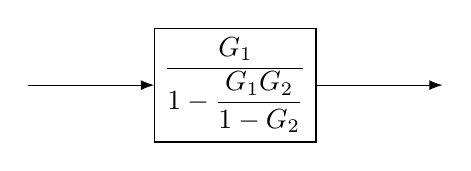
\begin{tikzpicture}[auto, node distance=1.0cm and 1.6cm, >=Latex]
    
      \node[input] (input) {};
      \node[block, right=of input] (final) {$\dfrac{G_1}{1 - \dfrac{G_1G_2}{1-G_2}}$};
      \node[output, right=of final] (output) {};
    
      \draw[->] (input) -- (final);
      \draw[->] (final) -- (output);
    
    \end{tikzpicture}

    \vspace{1.2em}
    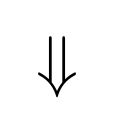
\begin{tikzpicture}
      \node {\Huge$\Downarrow$};
    \end{tikzpicture}
    \vspace{1.2em}
    
    % --- Step 4:全体を1つのブロックへ簡約2 ---
    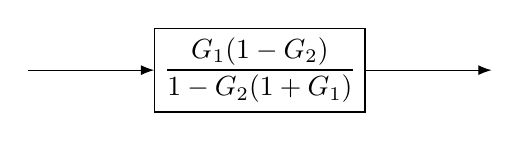
\begin{tikzpicture}[auto, node distance=1.0cm and 1.6cm, >=Latex]
    
      \node[input] (input) {};
      \node[block, right=of input] (final) {$\dfrac{G_1(1 - G_2)}{1 - G_2(1 + G_1)}$};
      \node[output, right=of final] (output) {};
    
      \draw[->] (input) -- (final);
      \draw[->] (final) -- (output);
    
    \end{tikzpicture}
    
    \end{center}
    
\end{tcolorbox}
% --------------- [41] --------------- 済
\begin{tcolorbox}[title={[41] 出力信号である制御量\(Y\)までの伝達特性を等価変換によって簡単化せよ.\\
    \qquad ただし、\(R\)は目標値信号,\(D\)は外乱信号である.
  \begin{center}
  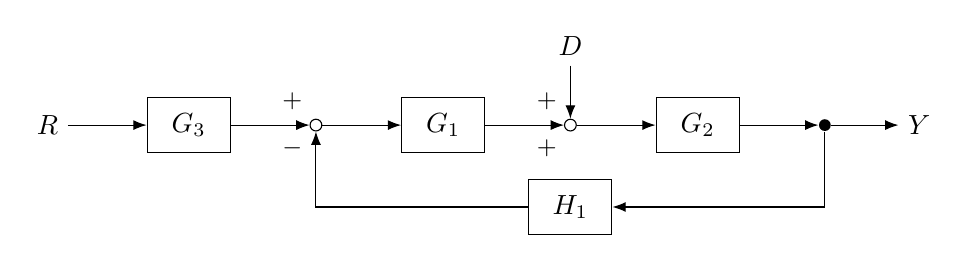
\begin{tikzpicture}[auto, node distance=0.8cm and 1.0cm, >=Latex]
  
    % --- ノードと信号配置(横並び) ---
    \node at (0,0) (R) {$R$};                           % R(目標値)
    \node[block, right=of R] (G3) {$G_3$};              % G3
    \node[circle, draw, inner sep=1.5pt, right=of G3] (sum1) {};  % 合流点1
    \node[block, right=of sum1] (G1) {$G_1$};           % G1
    \node[circle, draw, inner sep=1.5pt, right=of G1] (sum2) {};  % 合流点2
    \node[block, right=of sum2] (G2) {$G_2$};           % G2
    \node[circle, fill=black, inner sep=1.5pt, right=of G2] (branch) {}; % 分岐点
    \node at ($(branch)+(1.2,0)$) (Y) {$Y$};             % Y(制御量)
  
    % --- 上下ノード ---
    \node at ($(sum2)+(0,1.0)$) (D) {$D$};               % D(外乱)
    \node[block, below=0.6cm of sum2] (H1) {$H_1$};      % H1(下)
  
    % === 経路 ===
    \draw[->] (R) -- (G3);
    \draw[->] (G3) -- (sum1);
    \draw[->] (sum1) -- (G1);
    \draw[->] (G1) -- (sum2);
    \draw[->] (sum2) -- (G2);
    \draw[->] (G2) -- (branch);
    \draw[->] (branch) -- (Y);
  
    \draw[->] (D) -- (sum2);            % D → 合流点2
    \draw[->] (branch) |- (H1);         % 分岐 → H1(下)
    \draw[->] (H1) -| (sum1);           % H1 → 合流点1(戻る)
  
    % --- 加算記号配置 ---
    \node at ($(sum1)+(-0.3,0.3)$) {\small $+$};
    \node at ($(sum1)+(-0.3,-0.3)$) {\small $-$};
    \node at ($(sum2)+(-0.3,0.3)$) {\small $+$};
    \node at ($(sum2)+(-0.3,-0.3)$) {\small $+$};
  
  \end{tikzpicture}
  \end{center}
  }]
  %------- RからY -------
  RからYについて
  \begin{center}
  
    % --- Step 1:G₁とG₂のみを合成、G₃とH₁はそのまま配置 ---
    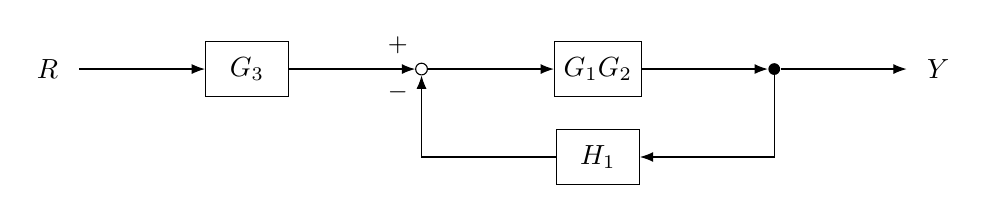
\begin{tikzpicture}[auto, node distance=1.2cm and 1.6cm, >=Latex]
    
      \node[input] (R) {};
      \node[block, right=of R] (G3) {$G_3$};
      \node[circle, draw, inner sep=1.5pt, right=of G3] (sum1) {};
      \node[block, right=of sum1] (G1G2) {$G_1 G_2$};
      \node[circle, fill=black, inner sep=1.5pt, right=of G1G2] (branch) {};
      \node[output, right=of branch] (Y) {};
    
      \node[block, below=0.4cm of G1G2] (H1) {$H_1$};
    
      \draw[->] (R) -- (G3);
      \draw[->] (G3) -- (sum1);
      \draw[->] (sum1) -- (G1G2);
      \draw[->] (G1G2) -- (branch);
      \draw[->] (branch) -- (Y);
    
      \draw[->] (branch) |- (H1);
      \draw[->] (H1) -| (sum1);
    
      \node at ($(sum1)+(-0.3,0.3)$) {\small $+$};
      \node at ($(sum1)+(-0.3,-0.3)$) {\small $-$};
      \node at ($(R)+(-0.4,0)$) {$R$};
      \node at ($(Y)+(0.4,0)$) {$Y$};
  
    
    \end{tikzpicture}
  
    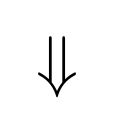
\begin{tikzpicture}
      \node {\Huge$\Downarrow$};
    \end{tikzpicture}
  
    
    % --- Step 2:H₁との負帰還構造を合成(G₃はまだ分離) ---
    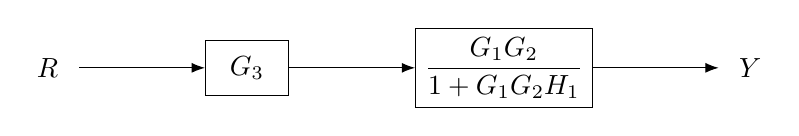
\begin{tikzpicture}[auto, node distance=1.2cm and 1.6cm, >=Latex]
    
      \node[input] (R) {};
      \node[block, right=of R] (G3) {$G_3$};
      \node[block, right=of G3] (closedLoop) {$\dfrac{G_1 G_2}{1 + G_1 G_2 H_1}$};
      \node[output, right=of closedLoop] (Y) {};
    
      \draw[->] (R) -- (G3);
      \draw[->] (G3) -- (closedLoop);
      \draw[->] (closedLoop) -- (Y);
  
      \node at ($(R)+(-0.4,0)$) {$R$};
      \node at ($(Y)+(0.4,0)$) {$Y$};
  
    
    \end{tikzpicture}
    
  
    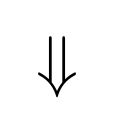
\begin{tikzpicture}
      \node {\Huge$\Downarrow$};
    \end{tikzpicture}
  
    
    % --- Step 3:G₃を含めた全体の1ブロック化 ---
    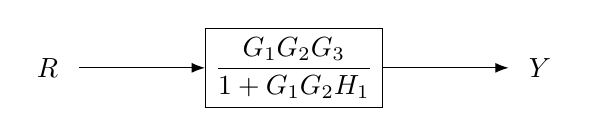
\begin{tikzpicture}[auto, node distance=1.4cm and 1.6cm, >=Latex]
    
      \node[input] (R) {};
      \node[block, right=of R] (total) {$\dfrac{G_1 G_2 G_3}{1 + G_1 G_2 H_1}$};
      \node[output, right=of total] (Y) {};
    
      \draw[->] (R) -- (total);
      \draw[->] (total) -- (Y);
  
      \node at ($(R)+(-0.4,0)$) {$R$};
      \node at ($(Y)+(0.4,0)$) {$Y$};
    
    \end{tikzpicture}
    
    \end{center}
  
  %------- DからY -------
  DからYについて
  \begin{center}
  
    % --- Step 0:G₂ → G₁ → 分岐 → H₁ → 合流点(D入力) ---
    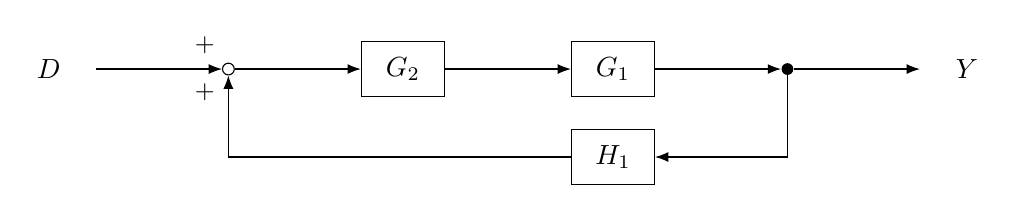
\begin{tikzpicture}[auto, node distance=1.2cm and 1.6cm, >=Latex]
    
      \node[input] (D) {};
      \node[circle, draw, inner sep=1.5pt, right=of D] (sum2) {};
      \node[block, right=of sum2] (G2) {$G_2$};
      \node[block, right=of G2] (G1) {$G_1$};
      \node[circle, fill=black, inner sep=1.5pt, right=of G1] (branch) {};
      \node[output, right=of branch] (Y) {};
      \node[block, below=0.4cm of G1] (H1) {$H_1$};
    
      \draw[->] (D) -- (sum2);
      \draw[->] (sum2) -- (G2);
      \draw[->] (G2) -- (G1);
      \draw[->] (G1) -- (branch);
      \draw[->] (branch) -- (Y);
    
      \draw[->] (branch) |- (H1);
      \draw[->] (H1) -| (sum2);
    
      \node at ($(D)+(-0.6,0)$) {$D$};
      \node at ($(Y)+(0.6,0)$) {$Y$};
      \node at ($(sum2)+(-0.3,0.3)$) {\small $+$};
      \node at ($(sum2)+(-0.3,-0.3)$) {\small $+$};
    
    \end{tikzpicture}
  
    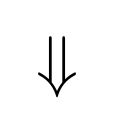
\begin{tikzpicture}
      \node {\Huge$\Downarrow$};
    \end{tikzpicture}
    
    % --- Step 1:G₁とG₂を合成(H₁と構造はそのまま) ---
    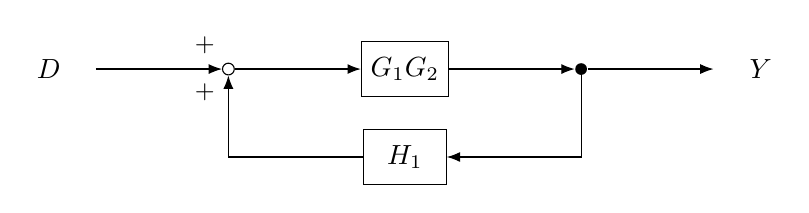
\begin{tikzpicture}[auto, node distance=1.2cm and 1.6cm, >=Latex]
    
      \node[input] (D) {};
      \node[circle, draw, inner sep=1.5pt, right=of D] (sum2) {};
      \node[block, right=of sum2] (G1G2) {$G_1 G_2$};
      \node[circle, fill=black, inner sep=1.5pt, right=of G1G2] (branch) {};
      \node[output, right=of branch] (Y) {};
      \node[block, below=0.4cm of G1G2] (H1) {$H_1$};
    
      \draw[->] (D) -- (sum2);
      \draw[->] (sum2) -- (G1G2);
      \draw[->] (G1G2) -- (branch);
      \draw[->] (branch) -- (Y);
    
      \draw[->] (branch) |- (H1);
      \draw[->] (H1) -| (sum2);
    
      \node at ($(D)+(-0.6,0)$) {$D$};
      \node at ($(Y)+(0.6,0)$) {$Y$};
      \node at ($(sum2)+(-0.3,0.3)$) {\small $+$};
      \node at ($(sum2)+(-0.3,-0.3)$) {\small $+$};
    
    \end{tikzpicture}
    
    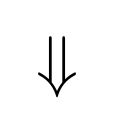
\begin{tikzpicture}
      \node {\Huge$\Downarrow$};
    \end{tikzpicture}
    
    % --- Step 2:全体を1ブロックに簡約(D→Y) ---
    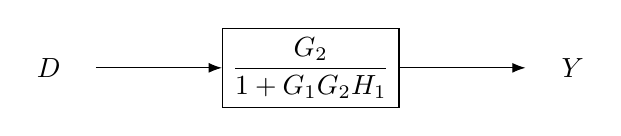
\begin{tikzpicture}[auto, node distance=1.4cm and 1.6cm, >=Latex]
    
      \node[input] (D) {};
      \node[block, right=of D] (total) {$\dfrac{G_2}{1 + G_1 G_2 H_1}$};
      \node[output, right=of total] (Y) {};
    
      \draw[->] (D) -- (total);
      \draw[->] (total) -- (Y);
    
      \node at ($(D)+(-0.6,0)$) {$D$};
      \node at ($(Y)+(0.6,0)$) {$Y$};
    
    \end{tikzpicture}
    
    \end{center}
  
    これらを合わせて
    \[
    Y=\frac{G_1 G_2 G_3 R + G_2 D}{1+G_1 G_2 H_1}\]
    
    
\end{tcolorbox}
% --------------- [42] --------------- 済
\begin{tcolorbox}[title={[42] \(a\)を入力,\(b\)を出力としたとき,ブロック線図を簡単化し,伝達関数を求めよ. 
\begin{center}
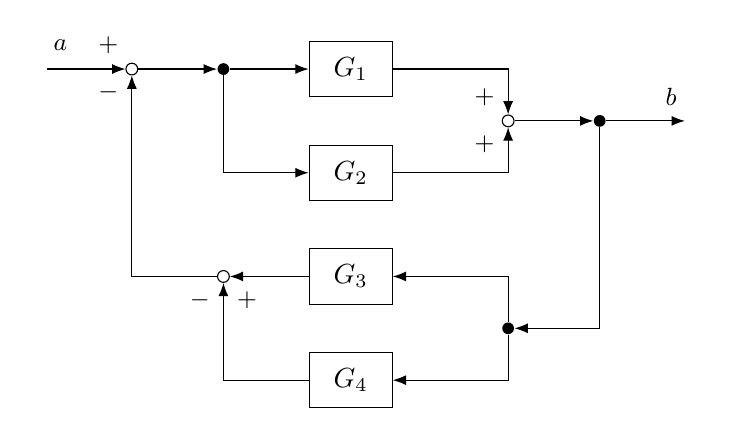
\begin{tikzpicture}[auto, node distance=0.8cm and 1.0cm, >=Latex]

% --- 上段:主系列ノード ---
\node at (0,0) (input) {};
\node[circle, draw, inner sep=1.5pt, right=of input] (sum1) {};               % 合流1
\node[circle, fill=black, inner sep=1.5pt, right=of sum1] (branch1) {};       % 分岐1
\node[block, right=of branch1] (G1) {$G_1$};                                   % G1

% --- 縦系列:G2〜G4 ---
\node[block, below=0.6cm of G1] (G2) {$G_2$};
\node[block, below=0.6cm of G2] (G3) {$G_3$};
\node[block, below=0.6cm of G3] (G4) {$G_4$};

% --- G1とG2の中間に sum2 → branch2 → output ---
\coordinate (mid12) at ($(G1)!0.5!(G2)$);
\node[circle, draw, inner sep=1.5pt] at ($(mid12)+(2.0,0)$) (sum2) {};        % 合流2
\node[circle, fill=black, inner sep=1.5pt, right=of sum2] (branch2) {};       % 分岐2
\node[right=of branch2] (output) {};

% --- G3とG4の中間に branch3 ---
\coordinate (mid34) at ($(G3)!0.5!(G4)$);
\node[circle, fill=black, inner sep=1.5pt] at ($(mid34)+(2.0,0)$) (branch3) {}; % 分岐3

% --- branch1の下かつG3の左に合流3 ---
\node[circle, draw, inner sep=1.5pt, left=of G3] (sum3) {};% 合流3

% === 経路 ===
\draw[->] (input) -- (sum1);
\draw[->] (sum1) -- (branch1);
\draw[->] (branch1) -- (G1);
\draw[->] (G1) -| (sum2);
\draw[->] (sum2) -- (branch2);
\draw[->] (branch2) -- (output);

\draw[->] (branch1) |- (G2);
\draw[->] (G2) -| (sum2);

\draw[->] (branch2) |- (branch3);
\draw[->] (branch3) |- (G3);
\draw[->] (G3) -- (sum3);
\draw[->] (sum3) -| (sum1);

\draw[->] (branch3) |- (G4);
\draw[->] (G4) -| (sum3);

% --- 加算記号 ---
\node at ($(sum1)+(-0.3,0.3)$) {\small $+$};
\node at ($(sum1)+(-0.3,-0.3)$) {\small $-$};
\node at ($(sum2)+(-0.3,0.3)$) {\small $+$};
\node at ($(sum2)+(-0.3,-0.3)$) {\small $+$};
\node at ($(sum3)+(-0.3,-0.3)$) {\small $-$};
\node at ($(sum3)+(0.3,-0.3)$) {\small $+$};

% --- その他記号 ---
\node at ($(input)+(0.3,0.3)$) {\small $a$};
\node at ($(output)+(-0.3,0.3)$) {\small $b$};

\end{tikzpicture}
\end{center}
}]

\begin{center}

    % --- Step 1:G₁+G₂,G₄−G₃ に合成した構造 ---
    \begin{tikzpicture}[auto, node distance=1.2cm and 1.8cm, >=Latex]

    \node[input] (input) {};
    \node[circle, draw, inner sep=1.5pt, right=of input] (sum1) {};
    \node[block, right=of sum1] (G1G2) {$G_1 + G_2$};
    \node[circle, fill=black, inner sep=1.5pt, right=of G1G2] (branch) {};
    \node[output, right=of branch] (output) {};
    \node[block, below=1.2cm of G1G2] (G3minusG4) {$G_3 - G_4$};
    
    \draw[->] (input) -- (sum1);
    \draw[->] (sum1) -- (G1G2);
    \draw[->] (G1G2) -- (branch);
    \draw[->] (branch) -- (output);
    
    \draw[->] (branch) |- (G3minusG4);
    \draw[->] (G3minusG4) -| (sum1);
    
    % ラベル配置
    \node at ($(input)+(0.3,0.3)$) {\small $a$};
    \node at ($(output)+(-0.3,0.3)$) {\small $b$};
    
    % 加算記号
    \node at ($(sum1)+(-0.3,0.3)$) {\small $+$};
    \node at ($(sum1)+(-0.3,-0.3)$) {\small $-$};
    
    \end{tikzpicture}
    
    \vspace{0.2cm}
    \begin{tikzpicture}
    \node {\Huge$\Downarrow$};
    \end{tikzpicture}
    \vspace{0.2cm}
    
    % --- Step 2:全体を1ブロックに簡約 ---
    \begin{tikzpicture}[auto, node distance=1.6cm and 1.6cm, >=Latex]
    
    \node[input] (a) {};
    \node[block, right=of a] (TF) {$\dfrac{G_1 + G_2}{1 + (G_1 + G_2)(G_3 - G_4)}$};
    \node[output, right=of TF] (b) {};
    
    \draw[->] (a) -- (TF);
    \draw[->] (TF) -- (b);
    
    \node at ($(a)+(0.3,0.3)$) {$a$};
    \node at ($(b)+(-0.3,0.3)$) {$b$};
    
    \end{tikzpicture}
    
    \end{center}
    

\end{tcolorbox}
% --------------- [43] --------------- 済
\begin{tcolorbox}[title={[43] 伝達関数\(\frac{b(s)}{a(s)}\)を求めよ. 
\begin{center}
\begin{tikzpicture}[auto, node distance=0.8cm and 1.0cm, >=Latex]

% --- 横並びノード ---
\node[circle, draw, inner sep=1.5pt] (sum) {};                  % 合流点
\node[block, right=of sum] (G) {$G(s)$};                        % G(s)
\node[circle, fill=black, inner sep=1.5pt, right=of G] (branch) {};  % 分岐点

% --- 下段ノード ---
\node[block, below=0.6cm of G] (H) {$H(s)$};                    % H(s)

% --- 経路 ---
\draw[->] ++(-1.2,0) -- (sum);              % input → 合流点
\draw[->] (sum) -- (G);                     % 合流点 → G(s)
\draw[->] (G) -- (branch);                  % G(s) → 分岐点
\draw[->] (branch) -- ++(1.0,0);            % 分岐点 → output

\draw[->] (branch) |- (H);                  % 分岐点 → H(s)
\draw[->] (H) -| (sum);                     % H(s) → 合流点

% --- 加算記号 ---
\node at ($(sum)+(-0.3,0.3)$) {\small $+$};
\node at ($(sum)+(-0.3,-0.3)$) {\small $-$};

% --- その他記号 ---
\node at ($(sum)+(-0.9,0.3)$) {\small $a(s)$};
\node at ($(sum)+(0.5,0.3)$) {\small $\varepsilon(s)$};
\node at ($(branch)+(0.5,0.3)$) {\small $b(s)$};
\node at ($(sum)+(-0.4,-0.9)$) {\small $c(s)$};
\end{tikzpicture}
\end{center}
}]

ブロック線図より次が成り立つ
\[
\left\{
\begin{aligned}
    \varepsilon(s) &=a(s) - c(s) \qquad \cdot \cdot \cdot (1)\\
    b(s) &=\varepsilon(s) G(s) \qquad \quad \cdot \cdot \cdot (2)\\
    c(s) &=b(s)H(s)\qquad \quad \cdot \cdot \cdot (3)\\
\end{aligned}
\right.
\]
であるから、最終的に\(\varepsilon(s),c(s)\)を含まない形にするために
\(\varepsilon(s)\)について解くと\\
\((1),(3)\)より
\begin{align*}
\varepsilon(s) &=a(s) - b(s)H(s)\qquad \quad \cdot \cdot \cdot (4)
\end{align*}
よって\((2),(4)\)より
\begin{align*}
    &\qquad \frac{b(s)}{G(s)} =\varepsilon(s) \\
    &\Leftrightarrow \frac{b(s)}{G(s)} =a(s) - b(s)H(s) \\
    &\Leftrightarrow b(s) = a(s)G(s)-b(s)H(s)G(s) \\
    &\Leftrightarrow b(s)\left\{1+G(s)H(s)\right\} = a(s)G(s) \\
    &\Leftrightarrow \frac{b(s)}{a(s)} = \frac{G(s)}{1+G(s)H(s)}
\end{align*}


\end{tcolorbox}
% --------------- [44] --------------- 済
\begin{tcolorbox}[title={[44] 二つの入力信号\(a_1(s),a_2(s)\)をもつ,制御系の応答\(b(s)\)を求めよ.
\begin{center}
\begin{tikzpicture}[auto, node distance=0.8cm and 1.0cm, >=Latex]

    % --- 上段ノード(横並び) ---
    \node[circle, draw, inner sep=1.5pt] (sum1) {};                % 合流点1
    \node[block, right=of sum1] (G1) {$G_2$};                      % G1
    \node[circle, fill=black, inner sep=1.5pt, right=of G1] (branch) {}; % 分岐点

    % input1とoutputの位置(描かない)
    \coordinate[left=of sum1] (input1);
    \coordinate[right=of branch] (output);

    % --- 中央の縦ノード(合流1 → G2 → 合流2) ---
    \node[block, below=0.8cm of sum1] (G2) {$G_1$};                % G2
    \node[circle, draw, inner sep=1.5pt, below=0.8cm of G2] (sum2) {}; % 合流点2

    % --- 下段(横並び) ---
    \coordinate[left=of sum2] (input2);                            % input2(描かない)
    \node[block, right=of sum2] (H) {$H$};                         % H

    % === 経路 ===
    \draw[->] (input1) -- (sum1);          % input1 → 合流点1
    \draw[->] (sum1) -- (G1);              % 合流点1 → G1
    \draw[->] (G1) -- (branch);            % G1 → 分岐点
    \draw[->] (branch) -- (output);        % 分岐点 → 出力

    \draw[->] (branch) |- (H);             % 分岐点 → H
    \draw[->] (H) -- (sum2);               % H → 合流点2
    \draw[->] (sum2) -- (G2);              % 合流点2 → G2
    \draw[->] (G2) -- (sum1);              % G2 → 合流点1

    \draw[->] (input2) -- (sum2);          % input2 → 合流点2

    % --- 加算記号配置 ---
    \node at ($(sum1)+(-0.3,0.3)$) {\small $+$};
    \node at ($(sum1)+(-0.3,-0.3)$) {\small $+$};
    \node at ($(sum2)+(-0.3,-0.3)$) {\small $+$};
    \node at ($(sum2)+(0.3,-0.3)$) {\small $-$};

    % --- その他記号配置 ---
    \node at ($(sum1)+(-1.0,0.3)$) {\small $a_2(s)$};
    \node at ($(sum2)+(-1.0,0.3)$) {\small $a_1(s)$};
    \node at ($(output)+(-0.3,0.3)$) {\small $b(s)$};

\end{tikzpicture}
\end{center}
}]

\(a_2(s)=0\)とおくと

\begin{center}
    \begin{tikzpicture}[auto, node distance=1.2cm and 1.6cm, >=Latex]
    
    \node[input] (a1) {};
    \node[circle, draw, inner sep=1.5pt, right=of a1] (sum) {};
    \node[block, right=of sum] (G1) {$G_1$};
    \node[block, right=of G1] (G2) {$G_2$};
    \node[circle, fill=black, inner sep=1.5pt, right=of G2] (branch) {};
    \node[output, right=of branch] (b1) {};
    
    \node[block] at ($(G1)!0.5!(G2)+(0,-1.2)$) (H) {$H$};
    
    \draw[->] (a1) -- (sum);
    \draw[->] (sum) -- (G1);
    \draw[->] (G1) -- (G2);
    \draw[->] (G2) -- (branch);
    \draw[->] (branch) -- (b1);
    
    \draw[->] (branch) |- (H);
    \draw[->] (H) -| (sum);
    
    \node at ($(a1)+(0.3,0.3)$) {\small $a_1(s)$};
    \node at ($(b1)+(-0.3,0.3)$) {\small $b_1(s)$};
    
    \node at ($(sum)+(-0.3,0.3)$) {\small $+$};
    \node at ($(sum)+(-0.3,-0.3)$) {\small $-$};
    
    \end{tikzpicture}
\end{center}

\[
b_1(s)=\frac{G_1G_2}{1+G_1G_2H} \cdot a_1(s) \qquad \cdot \cdot \cdot (1)
\]

\(a_2(s)=0\)とおくと

\begin{center}
    \begin{tikzpicture}[auto, node distance=1.6cm and 1.6cm, >=Latex]
    
    \node[input] (a1) {};
    \node[circle, draw, inner sep=1.5pt, right=of a1] (sum) {};
    \node[block, right=2.0cm of sum] (G2) {$G_2$};
    \node[circle, fill=black, inner sep=1.5pt, right=2.0cm of G2] (branch) {};
    \node[output, right=of branch] (b1) {};
    
    \node[block] at ($(G2)+(-1.2,-1.2)$) (G1) {$G_1$};
    \node[block] at ($(G2)+(1.2,-1.2)$) (H) {$H$};
    
    \draw[->] (a1) -- (sum);
    \draw[->] (sum) -- (G2);
    \draw[->] (G2) -- (branch);
    \draw[->] (branch) -- (b1);
    
    \draw[->] (branch) |- (H);
    \draw[->] (H) -- (G1);
    \draw[->] (G1) -| (sum);
    
    \node at ($(a1)+(0.3,0.3)$) {\small $a_2(s)$};
    \node at ($(b1)+(-0.3,0.3)$) {\small $b_2(s)$};
    
    \node at ($(sum)+(-0.3,0.3)$) {\small $+$};
    \node at ($(sum)+(-0.3,-0.3)$) {\small $-$};
    
    \end{tikzpicture}
\end{center}

\[
b_2(s)=\frac{G_2}{1+G_1G_2H} \cdot a_2(s) \qquad \cdot \cdot \cdot (2)
\]

以上\((1),(2)\)より

\begin{align*}
    b(s) & = b_1(s) + b_2(s)\\
        & = \frac{G_1 G_2 a_1(s)+G_2 a_2(s)}{1+G_1G_2H}
\end{align*}



\end{tcolorbox}
% --------------- [45] --------------- 済
\begin{tcolorbox}[title={[45] \(\frac{b_1(s)}{a_1(s)}\),\(\frac{b_1(s)}{a_2(s)}\),\(\frac{b_2(s)}{a_1(s)}\),\(\frac{b_2(s)}{a_2(s)}\)を求めよ. 
\vspace{-4mm}
\begin{center}
    \begin{tikzpicture}[auto, node distance=0.8cm and 1.0cm, >=Latex]

% === 上段主系列(横) ===
\coordinate (input1);
\node[circle, draw, inner sep=1.5pt, right=of input1] (sum1) {};           % 合流点1
\node[block, right=of sum1] (G1) {$G_1$};                                  % G1
\node[circle, fill=black, inner sep=1.5pt, right=of G1] (branch1) {};      % 分岐点1
\coordinate[right=of branch1] (output1);                                   % 出力1(描画しない)

% === sum1の下:G4 → branch2(縦) ===
\node[block, below=0.6cm of sum1] (G4) {$G_4$};
\node[circle, fill=black, inner sep=1.5pt, below=0.6cm of G4] (branch2) {}; % 分岐点2

% === branch1の下:G2 → sum2(縦) ===
\node[block, below=0.6cm of branch1] (G2) {$G_2$};
\node[circle, draw, inner sep=1.5pt, below=0.6cm of G2] (sum2) {};          % 合流点2

% === 下段横系列:output2 ← branch2 ← G3 ← sum2 ← input2 ===
\coordinate[left=of branch2] (output2);
\node[block, right=of branch2] (G3) {$G_3$};
\coordinate[right=of G3] (sum2_right);
\coordinate[right=of sum2_right] (input2);

% === 経路 ===
\draw[->] (input1) -- (sum1);             % input1 → sum1
\draw[->] (sum1) -- (G1);                 % sum1 → G1
\draw[->] (G1) -- (branch1);              % G1 → branch1
\draw[->] (branch1) -- (output1);         % branch1 → output1

\draw[->] (input2) -- (sum2);       % input2 → sum2(右から)
\draw[->] (sum2_right) -- (G3);           % → G3
\draw[->] (G3) -- (branch2);              % G3 → branch2
\draw[->] (branch2) -- (output2);         % branch2 → output2

\draw[->] (branch1) -- (G2);              % 分岐1 → G2
\draw[->] (G2) -- (sum2);                 % G2 → 合流2

\draw[->] (branch2) -- (G4);              % 分岐2 → G4
\draw[->] (G4) -- (sum1);                 % G4 → 合流1

% === 加算記号 ===
\node at ($(sum1)+(-0.3,0.3)$) {\small $+$};
\node at ($(sum1)+(-0.3,-0.3)$) {\small $-$};
\node at ($(sum2)+(0.3,0.3)$) {\small $-$};
\node at ($(sum2)+(0.3,-0.3)$) {\small $+$};

% === その他記号 ===
\node at ($(sum1)+(-1.0,0.3)$) {\small $a_1(s)$};
\node at ($(branch1)+(1.0,0.3)$) {\small $b_1(s)$};
\node at ($(sum2)+(1.0,-0.3)$) {\small $a_2(s)$};
\node at ($(branch2)+(-1.0,0.3)$) {\small $b_2(s)$};

    \end{tikzpicture}
\end{center}
}]

\(a_2(s)=0\)として
\vspace{-2mm}
\begin{center}
\begin{tikzpicture}[auto, node distance=0.8cm and 0.8cm, >=Latex]

    % --- 上段 ---
    \node[input] (a1) {};
    \node[circle, draw, inner sep=1.5pt, right=of a1] (sum1) {};
    \node[block, right=3.5cm of sum1] (G1) {$G_1$};
    \node[circle, fill=black, inner sep=1.5pt, right=3.5cm of G1] (branch) {};
    \node[output, right=of branch] (b1) {};

    % --- 下段 ---
    \node[block, below=0.4cm of G1] (G3) {$G_3$};
    \node[circle, draw, inner sep=1.5pt, right=0.6cm of G3] (sum2) {};
    \node[block, right=0.8cm of sum2] (G2) {$G_2$};
    \node[block, left=1.0cm of G3] (G4) {$G_4$};

    \draw[->] (a1) -- (sum1);
    \draw[->] (sum1) -- (G1);
    \draw[->] (G1) -- (branch);
    \draw[->] (branch) -- (b1);

    \draw[->] (branch) |- (G2);
    \draw[-] (G2) -- (sum2);
    \draw[->] (sum2) -- (G3);
    \draw[->] (G3) -- (G4);
    \draw[->] (G4) -| (sum1);

    % --- ラベル ---
    \node at ($(a1)+(-0.3,0.3)$) {\small $a_1(s)$};
    \node at ($(b1)+(0.3,0.3)$) {\small $b_1(s)$};

    % --- 加算記号 ---
    \node at ($(sum1)+(-0.3,0.3)$) {\small $+$};
    \node at ($(sum1)+(-0.3,-0.3)$) {\small $-$};
    \node at ($(sum2)+(0.3,0.3)$) {\small $-$};

\end{tikzpicture}
\end{center}

\[
\frac{b_1(s)}{a_1(s)}=\frac{1}{1-G_1 G_2 G_3 G_4}
\]

\begin{center}
    \begin{tikzpicture}[auto, node distance=1.6cm and 0.8cm, >=Latex]

    % 上段ノード
    \node[input] (a1) {};
    \node[circle, draw, inner sep=1.5pt, right=of a1] (sum1) {};
    \node[block, right=of sum1] (G1) {$G_1$};
    \node[block, right=of G1] (G2) {$G_2$};
    \node[circle, draw, inner sep=1.5pt, right=of G2] (sum2) {};
    \node[block, right=of sum2] (G3) {$G_3$};
    \node[circle, fill=black, inner sep=1.5pt, right=of G3] (branch) {};
    \node[output, right=of branch] (b2) {};

    % 下段ノード
    \node[block] at ($(G2)+(0.5,-1.2)$) (G4) {$G_4$};

    % 経路1:上段直線
    \draw[->] (a1) -- (sum1);
    \draw[->] (sum1) -- (G1);
    \draw[-] (G1) -- (G2);
    \draw[->] (G2) -- (sum2);
    \draw[->] (sum2) -- (G3);
    \draw[->] (G3) -- (branch);
    \draw[->] (branch) -- (b2);

    % 経路2:分岐 → G4 → sum1
    \draw[->] (branch) |- (G4);
    \draw[->] (G4) -| (sum1);

    % ラベル
    \node at ($(a1)+(-0.3,0.3)$) {\small $a_1(s)$};
    \node at ($(b2)+(0.3,0.3)$) {\small $b_2(s)$};

    % 加算記号
    \node at ($(sum1)+(-0.3,0.3)$) {\small $+$};
    \node at ($(sum1)+(-0.3,-0.3)$) {\small $-$};
    \node at ($(sum2)+(-0.3,0.3)$) {\small $-$};

    \end{tikzpicture}
\end{center}

\[
\frac{b_1(s)}{a_1(s)}=\frac{1}{1-G_1 G_2 G_3 G_4}
\]

\(a_1(s)=0\)として
\vspace{-2mm}
\begin{center}
    \begin{tikzpicture}[auto, node distance=1.6cm and 0.8cm, >=Latex]

    % 上段ノード
    \node[input] (a2) {};
    \node[circle, draw, inner sep=1.5pt, right=of a2] (sum2) {};
    \node[block, right=of sum2] (G3) {$G_3$};
    \node[block, right=of G3] (G4) {$G_4$};
    \node[circle, draw, inner sep=1.5pt, right=of G4] (sum1) {};
    \node[block, right=of sum1] (G1) {$G_1$};
    \node[circle, fill=black, inner sep=1.5pt, right=of G1] (branch) {};
    \node[output, right=of branch] (b1) {};

    % 下段ノード
    \node[block] at ($(G4)+(0.5,-1.2)$) (G2) {$G_2$};

    % 経路1(上段直線)
    \draw[->] (a2) -- (sum2);
    \draw[->] (sum2) -- (G3);
    \draw[->] (G3) -- (G4);
    \draw[-] (G4) -- (sum1);
    \draw[->] (sum1) -- (G1);
    \draw[->] (G1) -- (branch);
    \draw[->] (branch) -- (b1);

    % 経路2(分岐 → G2 → sum2)
    \draw[->] (branch) |- (G2);
    \draw[->] (G2) -| (sum2);

    % ラベル
    \node at ($(a2)+(-0.3,0.3)$) {\small $a_2(s)$};
    \node at ($(b1)+(0.3,0.3)$) {\small $b_1(s)$};

    % 加算記号
    \node at ($(sum2)+(0,0.3)$) {\small $+$};
    \node at ($(sum2)+(-0.3,-0.3)$) {\small $-$};
    \node at ($(sum1)+(0,0.3)$) {\small $-$};

    \end{tikzpicture}
\end{center}

\[
\frac{b_1(s)}{a_1(s)}=\frac{1}{1-G_1 G_2 G_3 G_4}
\]

\begin{center}
    \begin{tikzpicture}[auto, node distance=0.8cm and 0.8cm, >=Latex]

    % 上段:a2 → sum2 → G3 → branch → b2
    \node[input] (a2) {};
    \node[circle, draw, inner sep=1.5pt, right=of a2] (sum2) {};
    \node[block, right=3.5cm of sum2] (G3) {$G_3$};
    \node[circle, fill=black, inner sep=1.5pt, right=3.5cm of G3] (branch) {};
    \node[output, right=of branch] (b2) {};

    % 下段:G4 → sum1 → G1 → G2 → sum2
    \node[block] at ($(G3)+(2.2,-1.2)$) (G4) {$G_4$};
    \node[circle, draw, inner sep=1.5pt, left=0.8cm of G4] (sum1) {};
    \node[block, left=0.8cm of sum1] (G1) {$G_1$};
    \node[block, left=0.6cm of G1] (G2) {$G_2$};

    % 経路:上段
    \draw[->] (a2) -- (sum2);
    \draw[->] (sum2) -- (G3);
    \draw[->] (G3) -- (branch);
    \draw[->] (branch) -- (b2);

    % 経路:フィードバックルート
    \draw[->] (branch) |- (G4);
    \draw[-] (G4) -- (sum1);
    \draw[->] (sum1) -- (G1);
    \draw[->] (G1) -- (G2);
    \draw[->] (G2) -| (sum2);

    % ラベル
    \node at ($(a2)+(-0.3,0.3)$) {\small $a_2(s)$};
    \node at ($(b2)+(0.3,0.3)$) {\small $b_2(s)$};

    % 加算記号
    \node at ($(sum2)+(-0.3,0.3)$) {\small $+$};
    \node at ($(sum2)+(-0.3,-0.3)$) {\small $-$};
    \node at ($(sum1)+(0.3,0.3)$) {\small $-$};

    \end{tikzpicture}
\end{center} 

\[
\frac{b_1(s)}{a_1(s)}=\frac{1}{1-G_1 G_2 G_3 G_4}
\]



\end{tcolorbox}
% --------------- [46] --------------- 済
\begin{tcolorbox}[title={[46] ブロック線図を簡単にせよ.
\vspace{-12mm}
\begin{center}
\begin{tikzpicture}[auto, node distance=0.6cm and 0.8cm, >=Latex]

% --- 主系列ノード(横並び) ---
\coordinate (input);
\node[circle, draw, inner sep=1.5pt, right=of input] (sum1) {};        % 合流1
\node[block, right=of sum1] (G1) {$G_1$};                               % G1
\node[circle, draw, inner sep=1.5pt, right=of G1] (sum2) {};           % 合流2
\node[block, right=of sum2] (G2) {$G_2$};                               % G2
\node[circle, draw, inner sep=1.5pt, right=of G2] (sum3) {};           % 合流3
\node[block, right=of sum3] (G3) {$G_3$};                               % G3
\node[circle, fill=black, inner sep=1.5pt, right=of G3] (branch1) {};  % 分岐1
\node[block, right=of branch1] (G4) {$G_4$};                            % G4
\node[circle, fill=black, inner sep=1.5pt, right=of G4] (branch2) {};  % 分岐2
\coordinate[right=of branch2] (output);

% --- 上下ノード配置 ---
\node[block, above=1.2cm of branch1] (H2) {$H_2$};                      % H2(分岐1の上)
\node[block, below=of sum3] (H1) {$H_1$};                         % H1(合流3の下)
\node[circle, fill=black, inner sep=1.5pt] at ($(branch1)+(0,-1.1)$) (branch3) {};% 分岐3(分岐1の下)

% --- 経路①: input → ... → output ---
\draw[->] (input) -- (sum1);
\draw[->] (sum1) -- (G1);
\draw[->] (G1) -- (sum2);
\draw[->] (sum2) -- (G2);
\draw[->] (G2) -- (sum3);
\draw[->] (sum3) -- (G3);
\draw[->] (G3) -- (branch1);
\draw[->] (branch1) -- (G4);
\draw[->] (G4) -- (branch2);
\draw[->] (branch2) -- (output);

% --- 経路②: 分岐2 → H2 → 合流3 ---
\draw[->] (branch2) |- (H2);
\draw[->] (H2) -| (sum3);

% --- 経路③: 分岐1 → 分岐3 → H1 → 合流2 ---
\draw[->] (branch1) -- (branch3);
\draw[->] (branch3) -- (H1);
\draw[->] (H1) -| (sum2);

% --- 経路④: 分岐3 → ↓←↑ → 合流1 ---
\coordinate (pivot) at ($(sum1)+(0,-1.8)$); % 合流点1の下
\draw[->] (branch3) |-(pivot) -- (sum1);

% --- 加算記号配置 ---
\node at ($(sum1)+(-0.3,0.3)$) {\small $+$};
\node at ($(sum1)+(-0.3,-0.3)$) {\small $-$};
\node at ($(sum2)+(-0.3,0.3)$) {\small $+$};
\node at ($(sum2)+(-0.3,-0.3)$) {\small $+$};
\node at ($(sum3)+(-0.3,0.3)$) {\small $-$};
\node at ($(sum3)+(-0.3,-0.3)$) {\small $+$};

% --- その他記号配置 ---
\node at ($(sum1)+(-1.0,0.3)$) {\small $a(s)$};
\node at ($(branch2)+(1.0,0.3)$) {\small $b(s)$};

\end{tikzpicture}
\end{center}
\vspace{2mm}
}]

\begin{center}
    \begin{tikzpicture}[auto, node distance=0.4cm and 0.6cm, >=Latex]
    
    % === 中段(主系列) ===
    \node[input] (a) {};
    \node[circle, draw, inner sep=1.5pt, right=of a] (sum1) {};
    \node[block, right=of sum1] (G1) {$G_1$};
    \node[circle, draw, inner sep=1.5pt, right=of G1] (sum2) {};
    \node[block, right=of sum2] (G2) {$G_2$};
    \node[circle, draw, inner sep=1.5pt, right=of G2] (sum3) {};
    \node[block, right=1.6cm of sum3] (G3) {$G_3$};
    \node[circle, fill=black, inner sep=1.5pt, right=1.6cm of G3] (branch1) {};
    \node[block, right=0.8cm of branch1] (H4) {$G_4$};
    \node[output, right=of H4] (b) {};
    
    % === 上段(G4→H2) ===
    \node[block] at ($(branch1)+(-1.4,1.6)$) (G4) {$G_4$};
    \node[block, left=0.6cm of G4] (H2) {$H_2$};
    
    % === 下段(H1) ===
    \node[block] at ($(sum3)+(0,-1.6)$) (H1) {$H_1$};
    
    % === 経路(主系列) ===
    \draw[->] (a) -- (sum1);
    \draw[->] (sum1) -- (G1);
    \draw[->] (G1) -- (sum2);
    \draw[->] (sum2) -- (G2);
    \draw[->] (G2) -- (sum3);
    \draw[->] (sum3) -- (G3);
    \draw[->] (G3) -- (branch1);
    \draw[->] (branch1) -- (H4);
    \draw[->] (H4) -- (b);
    
    % === 経路:branch1 → G4 → H2 → sum3(上ループ)===
    \draw[->] (branch1) |- (G4);
    \draw[->] (G4) -- (H2);
    \draw[->] (H2) -| (sum3);
    
    % === 経路:branch1 → H1 → sum2(下ループ)===
    \draw[->] (branch1) |- (H1);
    \draw[->] (H1) -| (sum2);
    
    % === 経路:branch1 → sum1(フィードバック) ===
    \coordinate (pivot) at ($(sum1)+(0,-2.4)$);
    \draw[->] (branch1) |- (pivot) -- (sum1);
    
    % === ラベル ===
    \node at ($(a)+(-0.3,0.3)$) {\small $a(s)$};
    \node at ($(b)+(0.3,0.3)$) {\small $b(s)$};
    
    % === 加算記号 ===
    \node at ($(sum1)+(-0.3,0.3)$) {\small $+$};
    \node at ($(sum1)+(-0.3,-0.3)$) {\small $-$};
    \node at ($(sum2)+(-0.3,0.3)$) {\small $+$};
    \node at ($(sum2)+(-0.3,-0.3)$) {\small $+$};
    \node at ($(sum3)+(-0.3,0.3)$) {\small $-$};
    \node at ($(sum3)+(-0.3,-0.3)$) {\small $+$};
    
    \end{tikzpicture}

    \vspace{2mm}
    \begin{tikzpicture}
    \node {\Huge$\Downarrow$};
    \end{tikzpicture}
    \vspace{2mm}


\begin{tikzpicture}[auto, node distance=0.4cm and 0.6cm, >=Latex]

% 中段(主系列)
\node[input] (a) {};
\node[circle, draw, inner sep=1.5pt, right=of a] (sum1) {};
\node[block, right=of sum1] (G1) {$G_1$};
\node[circle, draw, inner sep=1.5pt, right=of G1] (sum2) {};
\node[block, right=of sum2] (G2) {$G_2$};
\node[block, right=1.6cm of G2] (G3combo) {$\dfrac{G_3}{1+G_3 G_4 H_2}$};
\node[circle, fill=black, inner sep=1.5pt, right=1.6cm of G3combo] (branch1) {};
\node[block, right=0.8cm of branch1] (G4) {$G_4$};
\node[output, right=of G4] (b) {};

% 下段:H1
\node[block] at ($(G2)+(1.0,-1.6)$) (H1) {$H_1$};

% 経路(主系列)
\draw[->] (a) -- (sum1);
\draw[->] (sum1) -- (G1);
\draw[->] (G1) -- (sum2);
\draw[->] (sum2) -- (G2);
\draw[->] (G2) -- (G3combo);
\draw[->] (G3combo) -- (branch1);
\draw[->] (branch1) -- (G4);
\draw[->] (G4) -- (b);

% 下段ループ
\draw[->] (branch1) |- (H1);
\draw[->] (H1) -| (sum2);

% フィードバック(sum1へ)
\coordinate (pivot) at ($(sum1)+(0,-2.4)$);
\draw[->] (branch1) |- (pivot) -- (sum1);

% ラベル
\node at ($(a)+(-0.3,0.3)$) {\small $a(s)$};
\node at ($(b)+(0.3,0.3)$) {\small $b(s)$};

% 加算記号
\node at ($(sum1)+(-0.3,0.3)$) {\small $+$};
\node at ($(sum1)+(-0.3,-0.3)$) {\small $-$};
\node at ($(sum2)+(-0.3,0.3)$) {\small $+$};
\node at ($(sum2)+(-0.3,-0.3)$) {\small $+$};

\end{tikzpicture}

    \vspace{2mm}
    \begin{tikzpicture}
    \node {\Huge$\Downarrow$};
    \end{tikzpicture}
    \vspace{2mm}

    \begin{tikzpicture}[auto, node distance=0.4cm and 0.6cm, >=Latex]
    
    % ノード配置
    \node[input] (a) {};
    \node[circle, draw, inner sep=1.5pt, right=of a] (sum1) {};
    \node[block, right=of sum1] (G1) {$G_1$};
    \node[block, right=of G1] (G2G3combo) 
        {$\dfrac{G_2 G_3}{1 + G_3 G_4 H_2 - G_2 G_3 H_1}$};
    \node[circle, fill=black, inner sep=1.5pt, right=1.8cm of G2G3combo] (branch1) {};
    \node[block, right=0.8cm of branch1] (G4final) {$G_4$};
    \node[output, right=of G4final] (b) {};
    
    % 経路
    \draw[->] (a) -- (sum1);
    \draw[->] (sum1) -- (G1);
    \draw[->] (G1) -- (G2G3combo);
    \draw[->] (G2G3combo) -- (branch1);
    \draw[->] (branch1) -- (G4final);
    \draw[->] (G4final) -- (b);
    
    % フィードバック:branch1 → sum1 (最終帰還)
    \coordinate (pivot1) at ($(sum1)+(0,-1.0)$);
    \draw[->] (branch1) |- (pivot1) -- (sum1);
    
    % ラベル
    \node at ($(a)+(-0.3,0.3)$) {\small $a(s)$};
    \node at ($(b)+(0.3,0.3)$) {\small $b(s)$};
    \node at ($(sum1)+(-0.3,0.3)$) {\small $+$};
    \node at ($(sum1)+(-0.3,-0.3)$) {\small $-$};
    
    \end{tikzpicture}

    \vspace{2mm}
    \begin{tikzpicture}
    \node {\Huge$\Downarrow$};
    \end{tikzpicture}
    \vspace{2mm}


    \begin{tikzpicture}[auto, node distance=0.4cm and 0.6cm, >=Latex]
    
    % ノード配置
    \node[input] (a) {};
    \node[block, right=of a] (core) 
        {$\dfrac{G_1 G_2 G_3}{1 + G_3 G_4 H_2 - G_2 G_3 H_1 + G_1 G_2 G_3}$};
    \node[block, right=of core] (G4) {$G_4$};
    \node[output, right=of G4] (b) {};
    
    % 経路
    \draw[->] (a) -- (core);
    \draw[->] (core) -- (G4);
    \draw[->] (G4) -- (b);
    
    % ラベル
    \node at ($(a)+(-0.3,0.3)$) {\small $a(s)$};
    \node at ($(b)+(0.3,0.3)$) {\small $b(s)$};
    
    \end{tikzpicture}

    \vspace{2mm}
    \begin{tikzpicture}
    \node {\Huge$\Downarrow$};
    \end{tikzpicture}
    \vspace{2mm}

    \vspace{2mm}
    \begin{tikzpicture}[auto, node distance=0.4cm and 0.6cm, >=Latex]
    
    \node[input] (a) {};
    \node[block, right=of a] (Gtotal) 
        {$\dfrac{G_1 G_2 G_3 G_4}{1 + G_3 G_4 H_2 - G_2 G_3 H_1 + G_1 G_2 G_3}$};
    \node[output, right=of Gtotal] (b) {};
    
    \draw[->] (a) -- (Gtotal);
    \draw[->] (Gtotal) -- (b);
    
    \node at ($(a)+(-0.3,0.3)$) {\small $a(s)$};
    \node at ($(b)+(0.3,0.3)$) {\small $b(s)$};
    
    \end{tikzpicture}
\end{center}







\end{tcolorbox}
% --------------- [47] --------------- 済
\begin{tcolorbox}[title={[47] ブロック線図を簡単にせよ. 
\begin{center}
    \begin{tikzpicture}[auto, node distance=0.8cm and 0.8cm, >=Latex]
    % --- 横並びの主系列ノード ---
    \node at (0,0) (input) {};
    \node[circle, draw, inner sep=1.5pt, right=of input] (sum1) {};           % 合流点1
    \node[block, right=of sum1] (G1) {$G_1$};
    \node[circle, draw, inner sep=1.5pt, right=of G1] (sum2) {};             % 合流点2
    \node[block, right=of sum2] (G2) {$G_2$};
    \node[circle, draw, inner sep=1.5pt, right=of G2] (sum3) {};             % 合流点3
    \node[block, right=of sum3] (G3) {$G_3$};
    \node[circle, fill=black, inner sep=1.5pt, right=of G3] (branch1) {};    % 分岐点1
    \node[block, right=of branch1] (G4) {$G_4$};
    \node[circle, fill=black, inner sep=1.5pt, right=of G4] (branch2) {};    % 分岐点2
    \node[right=of branch2] (output) {};
    
    % --- 分岐点3(branch2の下) ---
    \node[circle, fill=black, inner sep=1.5pt, below=1.0cm of branch2] (branch3) {};
    
    % === 主系列経路 ===
    \draw[->] (input) -- (sum1);
    \draw[->] (sum1) -- (G1);
    \draw[->] (G1) -- (sum2);
    \draw[->] (sum2) -- (G2);
    \draw[->] (G2) -- (sum3);
    \draw[->] (sum3) -- (G3);
    \draw[->] (G3) -- (branch1);
    \draw[->] (branch1) -- (G4);
    \draw[->] (G4) -- (branch2);
    \draw[->] (branch2) -- (output);
    
    % === 追加経路 ===
        % 分岐1 → 合流2(カクカク経路:下→左→上)
        \coordinate (pivot12) at ($(sum2)+(0,-0.7)$); 
        \draw[->] (branch1) |- (pivot12) -| (sum2);
    
        % 分岐2 → 分岐3(真下に新ノード) ←既に実装済
        \draw[->] (branch2) -- (branch3);
    
        % 分岐3 → 合流3(カクカク経路:下→左→上)
        \coordinate (pivot33) at ($(sum3)+(0,-1.2)$);
        \draw[->] (branch3) |- (pivot33) -| (sum3);              
    
    % 分岐3 → 合流1(カクカク:下→左→上、1本の矢印で)
    \coordinate (pivot) at ($(sum1)+(0,-1.8)$);
    \draw[->] (branch3) |- (pivot) -| (sum1);
    
    
    % --- 加算記号配置 ---
    \node at ($(sum1)+(-0.3,0.3)$) {\small $+$};
    \node at ($(sum1)+(-0.3,-0.3)$) {\small $-$};
    \node at ($(sum2)+(-0.3,0.3)$) {\small $+$};
    \node at ($(sum2)+(-0.3,-0.3)$) {\small $-$};
    \node at ($(sum3)+(-0.3,0.3)$) {\small $+$};
    \node at ($(sum3)+(-0.3,-0.3)$) {\small $-$};
    
    \node at ($(sum1)+(-1.0,0.3)$) {\small $R(s)$};
    \node at ($(branch2)+(1.0,0.3)$) {\small $C(s)$};
    
\end{tikzpicture}
\end{center}
\vspace{2mm}
}]

\begin{center}
    \begin{tikzpicture}[auto, node distance=0.8cm and 0.8cm, >=Latex]
    % --- 横並びの主系列ノード ---
    \node at (0,0) (input) {};
    \node[circle, draw, inner sep=1.5pt, right=of input] (sum1) {};           % 合流点1
    \node[block, right=of sum1] (G1) {$G_1$};
    \node[circle, draw, inner sep=1.5pt, right=of G1] (sum2) {};             % 合流点2
    \node[block, right=of sum2] (G2) {$G_2$};
    \node[circle, draw, inner sep=1.5pt, right=of G2] (sum3) {};             % 合流点3
    \node[block, right=of sum3] (G3) {$G_3$};
    \node[block, right=of G3] (G4) {$G_4$};
    \node[circle, fill=black, inner sep=1.5pt, right=of G4] (branch2) {};    % 分岐点2
    \node[right=of branch2] (output) {};
    
    % --- 分岐点3(branch2の下) ---
    \node[circle, fill=black, inner sep=1.5pt, below=0.9cm of branch2] (branch3) {};
    
    % --- 分岐点1(branch3の下) ---
    \node[circle, fill=black, inner sep=1.5pt, below=of branch3] (branch1) {};
    \node[block, left=1.6cm of branch1] (G4') {$\dfrac{1}{G_4}$};
    
    % === 主系列経路 ===
    \draw[->] (input) -- (sum1);
    \draw[->] (sum1) -- (G1);
    \draw[->] (G1) -- (sum2);
    \draw[->] (sum2) -- (G2);
    \draw[->] (G2) -- (sum3);
    \draw[->] (sum3) -- (G3);
    \draw[->] (G3) -- (G4);
    \draw[->] (G4) -- (branch2);
    \draw[->] (branch2) -- (output);
    
    % === 追加経路 ===
        % 分岐1 → 合流2(カクカク経路:上→左→上)
        \draw[->] (branch1) -- (G4') -| (sum2);
    
        % 分岐2 → 分岐3(真下に新ノード)
        \draw[->] (branch2) -- (branch3);
    
        % 分岐3 → 合流3(カクカク経路:下→左→上)
        \coordinate (pivot33) at ($(sum3)+(0,-1.0)$);
        \draw[->] (branch3) -- (pivot33) -| (sum3);              
    
        % 分岐3 → 合流1(カクカク:下→左→上、1本の矢印で)
        \coordinate (pivot) at ($(sum1)+(0,-2.8)$);
        \draw[->] (branch3) |- (pivot) -| (sum1);
    
    % --- 加算記号配置 ---
    \node at ($(sum1)+(-0.3,0.3)$) {\small $+$};
    \node at ($(sum1)+(-0.3,-0.3)$) {\small $-$};
    \node at ($(sum2)+(-0.3,0.3)$) {\small $+$};
    \node at ($(sum2)+(-0.3,-0.3)$) {\small $-$};
    \node at ($(sum3)+(-0.3,0.3)$) {\small $+$};
    \node at ($(sum3)+(-0.3,-0.3)$) {\small $-$};
    
    \node at ($(sum1)+(-1.0,0.3)$) {\small $R(s)$};
    \node at ($(branch2)+(1.0,0.3)$) {\small $C(s)$};
    
    \end{tikzpicture}


\vspace{2mm}
    \begin{tikzpicture}
    \node {\Huge$\Downarrow$};
    \end{tikzpicture}
\vspace{2mm}



\begin{tikzpicture}[auto, node distance=0.8cm and 0.8cm, >=Latex]
    % --- 横並びの主系列ノード ---
    \node at (0,0) (input) {};
    \node[circle, draw, inner sep=1.5pt, right=of input] (sum1) {};           % 合流点1
    \node[block, right=of sum1] (G1) {$G_1$};
    \node[circle, draw, inner sep=1.5pt, right=of G1] (sum2) {};             % 合流点2
    \node[block, right=of sum2] (G2) {$G_2$};           % 合流点3
    \node[block, right=of G2] (G34) {$\dfrac{G_3 G_4}{1 + G_3 G_4}$};       % 合成ブロック
    \node[circle, fill=black, inner sep=1.5pt, right=of G34] (branch2) {};   % 分岐点2
    \node[right=of branch2] (output) {};
    
    % --- 分岐点1(branch3の下) ---
    \node[circle, fill=black, inner sep=1.5pt, below=1.4cm of branch2] (branch1) {};
    \node[block, left=1.6cm of branch1] (G4inv) {$\dfrac{1}{G_4}$};

    % === 主系列経路 ===
    \draw[->] (input) -- (sum1);
    \draw[->] (sum1) -- (G1);
    \draw[->] (G1) -- (sum2);
    \draw[->] (sum2) -- (G2);
    \draw[->] (G2)  -- (G34);
    \draw[->] (G34) -- (branch2);
    \draw[->] (branch2) -- (output);

    % === 追加経路 ===
    % 分岐1 → 合流2(カクカク経路:上→左→上)
    \draw[->] (branch1) -- (G4inv) -| (sum2);

    % 分岐2 → 分岐3(真下に新ノード)
    \draw[->] (branch2) -- (branch1);

    % 分岐3 → 合流1(カクカク:下→左→上、1本の矢印で)
    \coordinate (pivot) at ($(sum1)+(0,-2.4)$);
    \draw[->] (branch1) |- (pivot) -| (sum1);

    % --- 加算記号配置 ---
    \node at ($(sum1)+(-0.3,0.3)$) {\small $+$};
    \node at ($(sum1)+(-0.3,-0.3)$) {\small $-$};
    \node at ($(sum2)+(-0.3,0.3)$) {\small $+$};
    \node at ($(sum2)+(-0.3,-0.3)$) {\small $-$};


    \node at ($(sum1)+(-1.0,0.3)$) {\small $R(s)$};
    \node at ($(branch2)+(1.0,0.3)$) {\small $C(s)$};

\end{tikzpicture}

\vspace{2mm}
    \begin{tikzpicture}
    \node {\Huge$\Downarrow$};
    \end{tikzpicture}
\vspace{2mm}


\begin{tikzpicture}[auto, node distance=0.8cm and 0.8cm, >=Latex]
    % --- 横並びの主系列ノード ---
    \node at (0,0) (input) {};
    \node[circle, draw, inner sep=1.5pt, right=of input] (sum1) {};                   % 合流点1
    \node[block, right=of sum1] (G1) {$G_1$};
    \node[block, right=of G1] (G234) {$\dfrac{G_2 G_3 G_4}{1 + G_2 G_3 + G_3 G_4}$};             % 合成ブロック
    \node[circle, fill=black, inner sep=1.5pt, right=of G234] (branch2) {};           % 分岐点2
    \node[right=of branch2] (output) {};

    % === 主系列経路 ===
    \draw[->] (input) -- (sum1);
    \draw[->] (sum1) -- (G1);
    \draw[->] (G1) -- (G234);
    \draw[->] (G234) -- (branch2);
    \draw[->] (branch2) -- (output);

    % === フィードバック(branch2 → sum1) ===
    \coordinate (pivot) at ($(sum1)+(0,-1.6)$);
    \draw[->] (branch2) |- (pivot) -| (sum1);

    % --- 加算記号配置 ---
    \node at ($(sum1)+(-0.3,0.3)$) {\small $+$};
    \node at ($(sum1)+(-0.3,-0.3)$) {\small $-$};

    \node at ($(sum1)+(-1.0,0.3)$) {\small $R(s)$};
    \node at ($(branch2)+(1.0,0.3)$) {\small $C(s)$};

\end{tikzpicture}

\vspace{2mm}
    \begin{tikzpicture}
    \node {\Huge$\Downarrow$};
    \end{tikzpicture}
\vspace{2mm}



\begin{tikzpicture}[auto, node distance=1.0cm and 1.5cm, >=Latex]
    % --- 入出力とブロック ---
    \node at (0,0) (input) {};
    \node[block, right=of input] (Gfinal) {$\dfrac{G_1 G_2 G_3 G_4}{1 + G_2 G_3 + G_3 G_4  + G_1 G_2 G_3 G_4}$};
    \node[right=of Gfinal] (output) {};
    
    % --- 矢印 ---
    \draw[->] (input) -- (Gfinal);
    \draw[->] (Gfinal) -- (output);
    
    % --- ラベル ---
    \node at ($(sum1)+(-1.0,0.3)$) {\small $R(s)$};
    \node at ($(branch2)+(1.0,0.3)$) {\small $C(s)$};
\end{tikzpicture}


\end{center}

\end{tcolorbox}
% --------------- [48] --------------- 済
\begin{tcolorbox}[title={[48] ブロック線図を簡単にせよ. 
\begin{center}
    \begin{tikzpicture}[auto, node distance=0.8cm and 1.2cm, >=Latex]

    % --- 横並びの主系列ノード ---
    \node at (0,0) (input) {};
    \node[circle, draw, inner sep=1.5pt, right=of input] (sum1) {};           % 合流点1
    \node[block, right=of sum1] (G1) {$G_1$};
    \node[circle, draw, inner sep=1.5pt, right=of G1] (sum2) {};             % 合流点2
    \node[block, right=of sum2] (G2) {$G_2$};
    \node[circle, fill=black, inner sep=1.5pt, right=of G2] (branch1) {};    % 分岐点1
    \node[right=of branch1] (output) {};                                     % 出力

    % --- 下部ノード配置 ---
    \node[circle, fill=black, inner sep=1.5pt, below=1.0cm of branch1] (branch2) {}; % 分岐点2
    \node[block, left=1.8cm of branch2] (H2) {$H_2$};                                 % H2
    \node[block, below=1.2cm of G1] (H1) {$H_1$};                                     % H1(H2より下)

    % === 主系列経路 ===
    \draw[->] (input) -- (sum1);
    \draw[->] (sum1) -- (G1);
    \draw[->] (G1) -- (sum2);
    \draw[->] (sum2) -- (G2);
    \draw[->] (G2) -- (branch1);
    \draw[->] (branch1) -- (output);

    % === 追加経路 ===
    % 分岐1 → 分岐2(真下)
    \draw[->] (branch1) -- (branch2);

    % 分岐2 → H2 → 合流点2(カクカク:左→上→右)

    \draw[->] (branch2) -- (H2);
    \draw[->] (H2) -| (sum2);

    % 分岐2 → H1 → 合流点1(カクカク:下→左→上)
    \draw[->] (branch2) |- (H1) -| (sum1);

    % --- 加算記号配置 ---
    \node at ($(sum1)+(-0.3,0.3)$) {\small $+$};
    \node at ($(sum1)+(-0.3,-0.3)$) {\small $-$};
    \node at ($(sum2)+(-0.3,0.3)$) {\small $+$};
    \node at ($(sum2)+(-0.3,-0.3)$) {\small $-$};

    % --- その他記号配置 ---
    \node at ($(sum1)+(-1.0,0.3)$) {\small $R(s)$};
    \node at ($(branch1)+(1.0,0.3)$) {\small $C(s)$};

\end{tikzpicture}
\end{center}
\vspace{2mm}
}]

\begin{center}
    \begin{tikzpicture}[auto, node distance=0.8cm and 1.2cm, >=Latex]
    
    % --- 横並びの主系列ノード ---
    \node at (0,0) (input) {};
    \node[circle, draw, inner sep=1.5pt, right=of input] (sum1) {};                  % 合流点1
    \node[block, right=of sum1] (G1) {$G_1$};
    \node[block, right=of G1] (G2H2) {$\dfrac{G_2}{1 + G_2 H_2}$};                   % フィードバック合成済ブロック
    \node[circle, fill=black, inner sep=1.5pt, right=of G2H2] (branch1) {};         % 分岐点1
    \node[right=of branch1] (output) {};                                            % 出力
    
    % --- 下部ノード(H1のみ) ---
    \node[block, below=1.2cm of G1] (H1) {$H_1$};
    
    % === 主系列経路 ===
    \draw[->] (input) -- (sum1);
    \draw[->] (sum1) -- (G1);
    \draw[->] (G1) -- (G2H2);
    \draw[->] (G2H2) -- (branch1);
    \draw[->] (branch1) -- (output);
    
    % === フィードバック H1 のみ ===
    \draw[->] (branch1) |- (H1) -| (sum1);
    
    % --- 加算記号配置 ---
    \node at ($(sum1)+(-0.3,0.3)$) {\small $+$};
    \node at ($(sum1)+(-0.3,-0.3)$) {\small $-$};
    
    % --- ラベル配置 ---
    \node at ($(sum1)+(-1.0,0.3)$) {\small $R(s)$};
    \node at ($(branch1)+(1.0,0.3)$) {\small $C(s)$};
    
    \end{tikzpicture}

    \vspace{2mm}
    \begin{tikzpicture}
    \node {\Huge$\Downarrow$};
    \end{tikzpicture}
\vspace{2mm}

    \begin{tikzpicture}[auto, node distance=1.5cm and 1.2cm, >=Latex]
    
    % --- ノード構成 ---
    \node at (0,0) (input) {};
    \node[block, right=of input] (Gfinal) {$\dfrac{G_1 G_2}{1 + G_2 H_2 + G_1 G_2 H_1}$};
    \node[right=of Gfinal] (output) {};
    
    % --- 主系列矢印 ---
    \draw[->] (input) -- (Gfinal);
    \draw[->] (Gfinal) -- (output);
    
    % --- 入出力ラベル ---
    \node at ($(input)+(0,0.3)$) {\small $R(s)$};
    \node at ($(output)+(0,0.3)$) {\small $C(s)$};
    
    \end{tikzpicture}
    
    
\end{center}
    


\end{tcolorbox}
% --------------- [49] --------------- 済
\begin{tcolorbox}[title={[49] ブロック線図を簡単にせよ. 
\begin{center}
    \begin{tikzpicture}[auto, node distance=0.8cm and 0.8cm, >=Latex]

    % --- 横並び:主系列ノード ---
    \node at (0,0) (input) {};
    \node[circle, draw, inner sep=1.5pt, right=of input] (sum1) {};         % 合流1
    \node[block, right=of sum1] (G1) {$G_1$};
    \node[circle, draw, inner sep=1.5pt, right=of G1] (sum2) {};            % 合流2
    \node[block, right=of sum2] (G2) {$G_2$};
    \node[circle, draw, inner sep=1.5pt, right=of G2] (sum3) {};            % 合流3
    \node[block, right=of sum3] (G3) {$G_3$};
    \node[circle, fill=black, inner sep=1.5pt, right=of G3] (branch1) {};   % 分岐1
    \node[block, right=of branch1] (G4) {$G_4$};
    \node[circle, fill=black, inner sep=1.5pt, right=of G4] (branch2) {};   % 分岐2
    \node[right=of branch2] (output) {};

    % --- 上・下ノード配置 ---
    \node[block, above=0.7cm of sum3] (H2) {$H_2$};                       % 合流3の上:H2
    \node[circle, fill=black, inner sep=1.5pt, below=1.0cm of branch2] (branch3) {}; % 分岐3
    \node[block, left=2.4cm of branch3] (H3) {$H_3$};                     % 分岐3の左
    \node[block, below=1.5cm of sum3] (H1) {$H_1$};                       % 合流3の下(H3より下)

    % === 主経路 ===
    \draw[->] (input) -- (sum1);
    \draw[->] (sum1) -- (G1);
    \draw[->] (G1) -- (sum2);
    \draw[->] (sum2) -- (G2);
    \draw[->] (G2) -- (sum3);
    \draw[->] (sum3) -- (G3);
    \draw[->] (G3) -- (branch1);
    \draw[->] (branch1) -- (G4);
    \draw[->] (G4) -- (branch2);
    \draw[->] (branch2) -- (output);

    % === 分岐ルート ===
    \draw[->] (branch1) |- (H2);              % 分岐1 → H2
    \draw[->] (H2) -| (sum2);                 % H2 → 合流2

    \draw[->] (branch2) -- (branch3);         % 分岐2 → 分岐3
    \draw[->] (branch3) -- (H3);              % 分岐3 → H3
    \draw[->] (H3) -| (sum3);                 % H3 → 合流3

    \draw[->] (branch3) |- (H1);              % 分岐3 → H1(下)
    \draw[->] (H1) -| (sum1);                 % H1 → 合流1

    % --- 加算記号配置 ---
    \node at ($(sum1)+(-0.3,0.3)$) {\small $+$};
    \node at ($(sum1)+(-0.3,-0.3)$) {\small $-$};

    \node at ($(sum2)+(-0.3,0.3)$) {\small $+$};
    \node at ($(sum2)+(+0.3,+0.3)$) {\small $-$};

    \node at ($(sum3)+(-0.3,0.3)$) {\small $+$};
    \node at ($(sum3)+(-0.3,-0.3)$) {\small $-$};

    % --- その他記号配置 ---
    \node at ($(sum1)+(-1.0,0.3)$) {\small $R(s)$};
    \node at ($(branch2)+(1.0,0.3)$) {\small $C(s)$};

\end{tikzpicture}
\end{center}
\vspace{2mm}
}]

\begin{center}
    \begin{tikzpicture}[auto, node distance=0.8cm and 0.8cm, >=Latex]
    
    % --- 横並び:主系列ノード ---
    \node at (0,0) (input) {};
    \node[circle, draw, inner sep=1.5pt, right=of input] (sum1) {};         
    \node[block, right=of sum1] (G1) {$G_1$};
    \node[circle, draw, inner sep=1.5pt, right=of G1] (sum2) {};            
    \node[block, right=of sum2] (G2) {$G_2$};
    \node[circle, draw, inner sep=1.5pt, right=of G2] (sum3) {};            
    \node[block, right=of sum3] (G3) {$G_3$};
    \node[block, right=of G3] (G4) {$G_4$};
    \node[circle, fill=black, inner sep=1.5pt, right=of G4] (branch2) {};   % ← 分岐1と統合
    \node[right=of branch2] (output) {};
    
    % --- 上・下ノード配置 ---
    \node[block, above=0.7cm of sum3] (H2divG4) {$\dfrac{H_2}{G_4}$};    % ← H2/G4(上)
    \node[circle, fill=black, inner sep=1.5pt, below=1.0cm of branch2] (branch3) {};
    \node[block, left=2.4cm of branch3] (H3) {$H_3$};
    \node[block, below=1.5cm of sum3] (H1) {$H_1$};
    
    % === 主経路 ===
    \draw[->] (input) -- (sum1);
    \draw[->] (sum1) -- (G1);
    \draw[->] (G1) -- (sum2);
    \draw[->] (sum2) -- (G2);
    \draw[->] (G2) -- (sum3);
    \draw[->] (sum3) -- (G3);
    \draw[->] (G3) -- (G4);
    \draw[->] (G4) -- (branch2);
    \draw[->] (branch2) -- (output);
    
    % === 分岐ルート ===
    \draw[->] (branch2) |- (H2divG4);      % 上:H2 / G4
    \draw[->] (H2divG4) -| (sum2);
    
    \draw[->] (branch2) -- (branch3);
    \draw[->] (branch3) -- (H3);
    \draw[->] (H3) -| (sum3);
    
    \draw[->] (branch3) |- (H1);
    \draw[->] (H1) -| (sum1);
    
    % --- 加算記号配置 ---
    \node at ($(sum1)+(-0.3,0.3)$) {\small $+$};
    \node at ($(sum1)+(-0.3,-0.3)$) {\small $-$};
    
    \node at ($(sum2)+(-0.3,0.3)$) {\small $+$};
    \node at ($(sum2)+(+0.3,+0.3)$) {\small $-$};
    
    \node at ($(sum3)+(-0.3,0.3)$) {\small $+$};
    \node at ($(sum3)+(-0.3,-0.3)$) {\small $-$};
    
    % --- ラベル配置 ---
    \node at ($(sum1)+(-1.0,0.3)$) {\small $R(s)$};
    \node at ($(branch2)+(1.0,0.3)$) {\small $C(s)$};
    
    \end{tikzpicture}


    \vspace{2mm}
    \begin{tikzpicture}
        \node {\Huge$\Downarrow$};
    \end{tikzpicture}
    \vspace{2mm}


    \begin{tikzpicture}[auto, node distance=0.8cm and 0.8cm, >=Latex]
    
    % --- 横並び:主系列ノード ---
    \node at (0,0) (input) {};
    \node[circle, draw, inner sep=1.5pt, right=of input] (sum1) {};         
    \node[block, right=of sum1] (G1) {$G_1$};
    \node[circle, draw, inner sep=1.5pt, right=of G1] (sum2) {};            
    \node[block, right=of sum2] (G2) {$G_2$};
    \node[block, right=of G2] (G34H3) {$\dfrac{G_3 G_4}{1 + G_3 G_4 H_3}$};  % 合成済ブロック
    \node[circle, fill=black, inner sep=1.5pt, right=of G34H3] (branch2) {};
    \node[right=of branch2] (output) {};
    
    % --- 上・下ノード配置 ---
    \node[block, above=0.6cm of G2] (H2divG4) {$\dfrac{H_2}{G_4}$};    % H₂/G₄(変更なし)
    \node[block, below=0.6cm of G1] (H1) {$H_1$};
    
    % === 主経路 ===
    \draw[->] (input) -- (sum1);
    \draw[->] (sum1) -- (G1);
    \draw[->] (G1) -- (sum2);
    \draw[->] (sum2) -- (G2);
    \draw[->] (G2) -- (G34H3);
    \draw[->] (G34H3) -- (branch2);
    \draw[->] (branch2) -- (output);
    
    % === 分岐ルート ===
    \draw[->] (branch2) |- (H2divG4);
    \draw[->] (H2divG4) -| (sum2);
    
    \draw[->] (branch2) |- (H1);
    \draw[->] (H1) -| (sum1);
    
    % --- 加算記号配置 ---
    \node at ($(sum1)+(-0.3,0.3)$) {\small $+$};
    \node at ($(sum1)+(-0.3,-0.3)$) {\small $-$};
    
    \node at ($(sum2)+(-0.3,0.3)$) {\small $+$};
    \node at ($(sum2)+(+0.3,+0.3)$) {\small $-$};
    
    % --- ラベル配置 ---
    \node at ($(sum1)+(-1.0,0.3)$) {\small $R(s)$};
    \node at ($(branch2)+(1.0,0.3)$) {\small $C(s)$};
    
    \end{tikzpicture}

    \vspace{2mm}
    \begin{tikzpicture}
        \node {\Huge$\Downarrow$};
    \end{tikzpicture}
    \vspace{2mm}


    \begin{tikzpicture}[auto, node distance=0.8cm and 0.8cm, >=Latex]
    
    % --- 横並び:主系列ノード ---
    \node at (0,0) (input) {};
    \node[circle, draw, inner sep=1.5pt, right=of input] (sum1) {};         
    \node[block, right=of sum1] (G1) {$G_1$};
    \node[block, right=of G1] (G234) {$\dfrac{G_2 G_3 G_4}{1 + G_3 G_4 H_3 + G_2 G_3 H_2}$}; % 合成済ブロック
    \node[circle, fill=black, inner sep=1.5pt, right=of G234] (branch2) {};
    \node[right=of branch2] (output) {};
    
    % --- 下ノード配置(H1のみ) ---
    \node[block, below=0.6cm of G1] (H1) {$H_1$};
    
    % === 主経路 ===
    \draw[->] (input) -- (sum1);
    \draw[->] (sum1) -- (G1);
    \draw[->] (G1) -- (G234);
    \draw[->] (G234) -- (branch2);
    \draw[->] (branch2) -- (output);
    
    % === フィードバック:H1のみ残す ===
    \draw[->] (branch2) |- (H1);
    \draw[->] (H1) -| (sum1);
    
    % --- 加算記号配置 ---
    \node at ($(sum1)+(-0.3,0.3)$) {\small $+$};
    \node at ($(sum1)+(-0.3,-0.3)$) {\small $-$};
    
    % --- ラベル配置 ---
    \node at ($(sum1)+(-1.0,0.3)$) {\small $R(s)$};
    \node at ($(branch2)+(1.0,0.3)$) {\small $C(s)$};
    
    \end{tikzpicture}

    \vspace{2mm}
    \begin{tikzpicture}
        \node {\Huge$\Downarrow$};
    \end{tikzpicture}
    \vspace{2mm}

    \begin{tikzpicture}[auto, node distance=1.5cm and 1.5cm, >=Latex]
    
    % --- ノード構成 ---
    \node at (0,0) (input) {};
    \node[block, right=of input] (Gfinal) {$\dfrac{G_1 G_2 G_3 G_4}{1 + G_3 G_4 H_3 + G_2 G_3 H_2 + G_1 G_2 G_3 G_4 H_1}$};
    \node[right=of Gfinal] (output) {};
    
    % --- 経路 ---
    \draw[->] (input) -- (Gfinal);
    \draw[->] (Gfinal) -- (output);
    
    % --- ラベル ---
    \node at ($(input)+(0,0.3)$) {\small $R(s)$};
    \node at ($(output)+(0,0.3)$) {\small $C(s)$};
    
    \end{tikzpicture}

    \end{center}





    
    

\end{tcolorbox}
% --------------- [50] --------------- 済
\begin{tcolorbox}[title={[50] ブロック線図を簡単にせよ. 
\vspace{-2mm}
\begin{center}
    \begin{tikzpicture}[auto, node distance=0.8cm and 0.8cm, >=Latex]

    % --- 横並びの主系列ノード ---
    \node at (0,0) (input) {};
    \node[circle, draw, inner sep=1.5pt, right=of input] (sum1) {};         % 合流1
    \node[block, right=of sum1] (G1) {$G_1$};
    \node[circle, draw, inner sep=1.5pt, right=of G1] (sum2) {};            % 合流2
    \node[block, right=of sum2] (G2) {$G_2$};
    \node[circle, fill=black, inner sep=1.5pt, right=of G2] (branch1) {};   % 分岐1
    \node[block, right=of branch1] (G3) {$G_3$};
    \node[circle, fill=black, inner sep=1.5pt, right=of G3] (branch2) {};   % 分岐2
    \node[right=of branch2] (output) {};
    
    % --- 合流3(sum1の下) ---
    \node[circle, draw, inner sep=1.5pt, below=0.7cm of sum1] (sum3) {};    % 合流3
    
    % === 経路 ===
    \draw[->] (input) -- (sum1);
    \draw[->] (sum1) -- (G1);
    \draw[->] (G1) -- (sum2);
    \draw[->] (sum2) -- (G2);
    \draw[->] (G2) -- (branch1);
    \draw[->] (branch1) -- (G3);
    \draw[->] (G3) -- (branch2);
    \draw[->] (branch2) -- (output);
    
    \draw[->] (branch1) |- (sum3);      % 分岐1 → 合流3
    \draw[->] (sum3) -- (sum1);         % 合流3 → 合流1
    
    \draw[->] (branch2) |- ++(0,-1.5) -| (sum3);   % 分岐2 → 合流3(下経路)
    \draw[->] (branch2) |- ++(0,0.8) -| (sum2);    % 分岐2 → 合流2(上経路)
    
    % --- 加算記号配置 ---
    \node at ($(sum1)+(-0.3,0.3)$) {\small $+$};
    \node at ($(sum1)+(-0.3,-0.3)$) {\small $-$};
    \node at ($(sum2)+(-0.3,0.3)$) {\small $+$};
    \node at ($(sum2)+(0.3,0.3)$) {\small $-$};
    \node at ($(sum3)+(0.3,0.3)$) {\small $+$};
    \node at ($(sum3)+(-0.3,-0.3)$) {\small $+$};
    
    % --- その他記号配置 ---
    \node at ($(sum1)+(-0.8,0.3)$) {\small $u$};
    \node at ($(branch2)+(0.8,0.3)$) {\small $y$};
    
\end{tikzpicture}
\end{center}
\vspace{1mm}
}]

\begin{center}
    \begin{tikzpicture}[auto, node distance=0.8cm and 0.8cm, >=Latex]
    
    % --- 横並び:主系列ノード ---
    \node at (0,0) (input) {};
    \node[circle, draw, inner sep=1.5pt, right=of input] (sum1) {};         % 合流1
    \node[block, right=of sum1] (G1) {$G_1$};
    \node[circle, draw, inner sep=1.5pt, right=of G1] (sum2) {};            % 合流2
    \node[block, right=of sum2] (G2) {$G_2$};
    \node[block, right=of G2] (G3) {$G_3$};
    \node[circle, fill=black, inner sep=1.5pt, right=of G3] (branch1) {};   % 分岐1をG3の右に移動
    \node[circle, fill=black, inner sep=1.5pt, right=of branch1] (branch2) {}; 
    \node[right=of branch2] (output) {};
    
    % --- 合流3(sum1の下) ---
    \node[circle, draw, inner sep=1.5pt, below=1.15cm of sum1] (sum3) {};    % 合流3
    
    % --- G2の下に 1/G3 ノード追加 ---
    \node[block, below=0.3cm of G2] (invG3) {$\dfrac{1}{G_3}$};
    
    % === 主系列 ===
    \draw[->] (input) -- (sum1);
    \draw[->] (sum1) -- (G1);
    \draw[->] (G1) -- (sum2);
    \draw[->] (sum2) -- (G2);
    \draw[->] (G2) -- (G3);
    \draw[->] (G3) -- (branch1);
    \draw[->] (branch1) -- (branch2);
    \draw[->] (branch2) -- (output);
    
    % === 分岐ルート(新しい分岐1 → 1/G3 → 合流3)===
    \draw[->] (branch1) |- (invG3);
    \draw[->] (invG3) -- (sum3);
    \draw[->] (sum3) -- (sum1);
    
    % === 既存の分岐2からのフィードバックルート ===
    \draw[->] (branch2) |- ++(0,-2.2) -| (sum3);   % 分岐2 → 合流3(下経路)
    \draw[->] (branch2) |- ++(0,1.2) -| (sum2);    % 分岐2 → 合流2(上経路)
    
    % --- 加算記号配置 ---
    \node at ($(sum1)+(-0.3,0.3)$) {\small $+$};
    \node at ($(sum1)+(-0.3,-0.3)$) {\small $-$};
    
    \node at ($(sum2)+(-0.3,0.3)$) {\small $+$};
    \node at ($(sum2)+(0.3,0.3)$) {\small $-$};
    
    \node at ($(sum3)+(0.3,0.3)$) {\small $+$};
    \node at ($(sum3)+(-0.3,-0.3)$) {\small $+$};
    
    % --- ラベル配置 ---
    \node at ($(sum1)+(-0.8,0.3)$) {\small $u$};
    \node at ($(branch2)+(0.8,0.3)$) {\small $y$};
    
    \end{tikzpicture}


\vspace{2mm}
    \begin{tikzpicture}
    \node {\Huge$\Downarrow$};
    \end{tikzpicture}
\vspace{2mm}


    \begin{tikzpicture}[auto, node distance=0.8cm and 0.8cm, >=Latex]
    
    % --- 横並び:主系列ノード ---
    \node at (0,0) (input) {};
    \node[circle, draw, inner sep=1.5pt, right=of input] (sum1) {};         
    \node[block, right=of sum1] (G1) {$G_1$};
    \node[circle, draw, inner sep=1.5pt, right=of G1] (sum2) {};            
    \node[block, right=of sum2] (G2) {$G_2$};
    \node[block, right=of G2] (G3) {$G_3$};
    \node[circle, fill=black, inner sep=1.5pt, right=of G3] (branch2) {}; 
    \node[right=of branch2] (output) {};
    
    % --- 新しいフィードバックブロック(1 + 1/G3) ---
    \node[block, below=0.8cm of G2] (feedback) {$1 + \dfrac{1}{G_3}$};
    
    % === 主系列 ===
    \draw[->] (input) -- (sum1);
    \draw[->] (sum1) -- (G1);
    \draw[->] (G1) -- (sum2);
    \draw[->] (sum2) -- (G2);
    \draw[->] (G2) -- (G3);
    \draw[->] (G3) -- (branch2);
    \draw[->] (branch2) -- (output);
    
    % === 合成済みフィードバックルート ===
    \draw[->] (branch2) |- (feedback);
    \draw[->] (feedback) -| (sum1);
    
    % === 残るフィードバック(上) ===
    \draw[->] (branch2) |- ++(0,1.2) -| (sum2);
    
    % --- 加算記号配置 ---
    \node at ($(sum1)+(-0.3,0.3)$) {\small $+$};
    \node at ($(sum1)+(-0.3,-0.3)$) {\small $-$};
    
    \node at ($(sum2)+(-0.3,0.3)$) {\small $+$};
    \node at ($(sum2)+(0.3,0.3)$) {\small $-$};
    
    % --- ラベル配置 ---
    \node at ($(sum1)+(-0.8,0.3)$) {\small $u$};
    \node at ($(branch2)+(0.8,0.3)$) {\small $y$};
    
    \end{tikzpicture}


\vspace{2mm}
    \begin{tikzpicture}
    \node {\Huge$\Downarrow$};
    \end{tikzpicture}
\vspace{2mm}


    \begin{tikzpicture}[auto, node distance=0.8cm and 0.8cm, >=Latex]
    
        % --- 横並び:主系列ノード ---
        \node at (0,0) (input) {};
        \node[circle, draw, inner sep=1.5pt, right=of input] (sum1) {};
        \node[block, right=of sum1] (G1) {$G_1$};
        \node[block, right=of G1] (G23fb) {$\dfrac{G_2 G_3}{1 + G_2 G_3}$}; % 合成ブロック
        \node[circle, fill=black, inner sep=1.5pt, right=of G23fb] (branch2) {};
        \node[right=of branch2] (output) {};
    
        % --- フィードバックブロック(1 + 1/G₃) ---
        \node[block, below=0.8cm of G23fb] (feedback) {$1 + \dfrac{1}{G_3}$};
    
        % === 主系列 ===
        \draw[->] (input) -- (sum1);
        \draw[->] (sum1) -- (G1);
        \draw[->] (G1) -- (G23fb);
        \draw[->] (G23fb) -- (branch2);
        \draw[->] (branch2) -- (output);
    
        % === フィードバック(下) ===
        \draw[->] (branch2) |- (feedback);
        \draw[->] (feedback) -| (sum1);
    
        % --- 加算記号配置 ---
        \node at ($(sum1)+(-0.3,0.3)$) {\small $+$};
        \node at ($(sum1)+(-0.3,-0.3)$) {\small $-$};
    
        % --- ラベル配置 ---
        \node at ($(sum1)+(-0.8,0.3)$) {\small $u$};
        \node at ($(branch2)+(0.8,0.3)$) {\small $y$};
    
    \end{tikzpicture}

\vspace{2mm}
    \begin{tikzpicture}
    \node {\Huge$\Downarrow$};
    \end{tikzpicture}
\vspace{2mm}

    \begin{tikzpicture}[auto, node distance=1.5cm and 1.5cm, >=Latex]
    
    % --- ノード構成 ---
    \node at (0,0) (input) {};
    \node[block, right=of input] (Gfinal) {$\dfrac{G_1 G_2 G_3}{1 + G_2 G_3 + G_1 G_2 G_3 + G_1 G_2}$};
    \node[right=of Gfinal] (output) {};
    
    % --- 経路 ---
    \draw[->] (input) -- (Gfinal);
    \draw[->] (Gfinal) -- (output);
    
    % --- ラベル ---
    \node at ($(input)+(0.3,0.3)$) {\small $u$};
    \node at ($(output)+(-0.3,0.3)$) {\small $y$};
    
    \end{tikzpicture}

\end{center}


    \vspace{-2mm}
最後の変形について
    \begin{align*}
    \frac{G_1 \cdot \dfrac{G_2 G_3}{1 + G_2 G_3}}{1 + G_1 \cdot \dfrac{G_2 G_3}{1 + G_2 G_3} \cdot \left(1 + \dfrac{1}{G_3} \right)}
    &= \frac{G_1 G_2 G_3}{1 + G_2 G_3 + G_1 G_2 G_3 \left(1 + \dfrac{1}{G_3} \right)} \\[1ex]
    &= \frac{G_1 G_2 G_3}{1 + G_2 G_3 + G_1 G_2 + G_1 G_2 G_3}
    \end{align*}

\end{tcolorbox}

\end{document}

